% -*- Mode:TeX -*-

%% IMPORTANT: The official thesis specifications are available at:
%%            http://libraries.mit.edu/archives/thesis-specs/
%%
%%            Please verify your thesis' formatting and copyright
%%            assignment before submission. If you notice any
%%            discrepancies between these templates and the 
%%            MIT Libraries' specs, please let us know
%%            by e-mailing thesis@mit.edu

%% The documentclass options along with the pagestyle can be used to generate
%% a technical report, a draft copy, or a regular thesis. You may need to
%% re-specify the pagestyle after you \include cover.tex. For more
%% information, see the first few lines of mitthesis.cls. 

%\documentclass[12pt,vi,twoside]{mitthesis}
%%
%%  If you want your thesis copyright to you instead of MIT, use the
%%  ``vi'' option, as above.
%%
%\documentclass[12pt,twoside,leftblank]{mitthesis}
%%
%% If you want blank pages before new chapters to be labelled ``This
%% Page Intentionally Left Blank'', use the ``leftblank'' option, as
%% above. 

\documentclass[12pt,twoside]{mitthesis}
\usepackage{lgrind}
%% These have been added at the request of the MIT Libraries, because
%% some PDF conversions mess up the ligatures.  -LB, 1/22/2014
\usepackage{cmap}
\usepackage[T1]{fontenc}
\pagestyle{plain}

% ABF custom packages
\usepackage{xcolor}
\usepackage{graphicx}
\usepackage{float}
\newcommand\todo[1]{\textcolor{red}{#1}}

%% This bit allows you to either specify only the files which you wish to
%% process, or `all' to process all files which you \include.
%% Krishna Sethuraman (1990).

%\typein [\files]{Enter file names to process, (chap1,chap2 ...), or `all' to process all files:}
\def\all{all}
\ifx\files\all \typeout{Including all files.} \else %\typeout{Including only \files.} \includeonly{\files} \fi

\begin{document}

% -*-latex-*-
% 
% For questions, comments, concerns or complaints:
% thesis@mit.edu
% 
%
% $Log: cover.tex,v $
% Revision 1.9  2019/08/06 14:18:15  cmalin
% Replaced sample content with non-specific text.
%
% Revision 1.8  2008/05/13 15:02:15  jdreed
% Degree month is June, not May.  Added note about prevdegrees.
% Arthur Smith's title updated
%
% Revision 1.7  2001/02/08 18:53:16  boojum
% changed some \newpages to \cleardoublepages
%
% Revision 1.6  1999/10/21 14:49:31  boojum
% changed comment referring to documentstyle
%
% Revision 1.5  1999/10/21 14:39:04  boojum
% *** empty log message ***
%
% Revision 1.4  1997/04/18  17:54:10  othomas
% added page numbers on abstract and cover, and made 1 abstract
% page the default rather than 2.  (anne hunter tells me this
% is the new institute standard.)
%
% Revision 1.4  1997/04/18  17:54:10  othomas
% added page numbers on abstract and cover, and made 1 abstract
% page the default rather than 2.  (anne hunter tells me this
% is the new institute standard.)
%
% Revision 1.3  93/05/17  17:06:29  starflt
% Added acknowledgements section (suggested by tompalka)
% 
% Revision 1.2  92/04/22  13:13:13  epeisach
% Fixes for 1991 course 6 requirements
% Phrase "and to grant others the right to do so" has been added to 
% permission clause
% Second copy of abstract is not counted as separate pages so numbering works
% out
% 
% Revision 1.1  92/04/22  13:08:20  epeisach

% NOTE:
% These templates make an effort to conform to the MIT Thesis specifications,
% however the specifications can change. We recommend that you verify the
% layout of your title page with your thesis advisor and/or the MIT 
% Libraries before printing your final copy.
\title{Microarchitecture Categorization and Pre-RTL Analytical Modeling for Sparse Tensor Accelerators}

\author{Andrew Feldman}
% If you wish to list your previous degrees on the cover page, use the 
% previous degrees command:
\prevdegrees{S.B. in Electrical Engineering and Computer Science \\ Massachusetts Institute of Technology (2016)}
% You can use the \\ command to list multiple previous degrees
%       \prevdegrees{B.S., University of California (1978) \\
%                    S.M., Massachusetts Institute of Technology (1981)}
\department{Department of Electrical Engineering and Computer Science}

% If the thesis is for two degrees simultaneously, list them both
% separated by \and like this:
% \degree{Doctor of Philosophy \and Master of Science}
\degree{Master of Engineering in Electrical Engineering and Computer Science}

% As of the 2007-08 academic year, valid degree months are September, 
% February, or June.  The default is June.
\degreemonth{February}
\degreeyear{2024}
\thesisdate{\today}

%% By default, the thesis will be copyrighted to MIT.  If you need to copyright
%% the thesis to yourself, just specify the `vi' documentclass option.  If for
%% some reason you want to exactly specify the copyright notice text, you can
%% use the \copyrightnoticetext command.  
%\copyrightnoticetext{\copyright IBM, 1990.  Do not open till Xmas.}

% If there is more than one supervisor, use the \supervisor command
% once for each.
\supervisor{Vivienne Sze}{Associate Professor}
\supervisor{Joel Emer}{Professor of the Practice}

% This is the department committee chairman, not the thesis committee
% chairman.  You should replace this with your Department's Committee
% Chairman.
\chairman{Katrina LaCurts}{Chair, Master of Engineering Thesis Committee}

% Make the titlepage based on the above information.  If you need
% something special and can't use the standard form, you can specify
% the exact text of the titlepage yourself.  Put it in a titlepage
% environment and leave blank lines where you want vertical space.
% The spaces will be adjusted to fill the entire page.  The dotted
% lines for the signatures are made with the \signature command.
\maketitle

% The abstractpage environment sets up everything on the page except
% the text itself.  The title and other header material are put at the
% top of the page, and the supervisors are listed at the bottom.  A
% new page is begun both before and after.  Of course, an abstract may
% be more than one page itself.  If you need more control over the
% format of the page, you can use the abstract environment, which puts
% the word "Abstract" at the beginning and single spaces its text.

%% You can either \input (*not* \include) your abstract file, or you can put
%% the text of the abstract directly between the \begin{abstractpage} and
%% \end{abstractpage} commands.

% First copy: start a new page, and save the page number.
\cleardoublepage
% Uncomment the next line if you do NOT want a page number on your
% abstract and acknowledgments pages.
% \pagestyle{empty}
\setcounter{savepage}{\thepage}
\begin{abstractpage}
% $Log: abstract.tex,v $
% Revision 1.1  93/05/14  14:56:25  starflt
% Initial revision
% 
% Revision 1.1  90/05/04  10:41:01  lwvanels
% Initial revision
% 
%
%% The text of your abstract and nothing else (other than comments) goes here.
%% It will be single-spaced and the rest of the text that is supposed to go on
%% the abstract page will be generated by the abstractpage environment.  This
%% file should be \input (not \include 'd) from cover.tex.

% , utilizing simple formulae for \textit{architectural} compute and memory savings from sparse acceleration features (SAFs.) 

Specialized microarchitectures for exploiting sparsity have critical to the design of sparse tensor accelerators. Despite considerable research having been done, prior work lacks consistent abstractions, systematic design-space exploration, and apples-to-apples comparison between alternative microarchitecture proposals.

Sparseloop (in combination with the Accelergy modeling framework) is an example of an existing tool which attempts to analytically model sparsity optimizations, known as Sparse Acceleration Features (SAFs.) Sparseloop effectively models key metrics such as energy, area and cycles at the architecture-level in the presence of sparsity optimizations. However, lacking models of microarchitectural primitives and design topologies, Sparseloop is unable to lower its sparsity abstractions onto a model of microarchitectural costs. Thus Sparseloop cannot capture the energy/area/time overhead incurred by SAF microarchitectures.

This work attempts to synthesize a number of prior works into a concise, unified, and effective framework for doing research on SAF microarchitectures. This overall framework comprises (1) a conceptual framework which facilitates concise description and design-space exploration for SAF microarchitectures, (2) a software framework for compiling Sparseloop-style SAF descriptions into microarchitecture designs and analytical models, and (3) a component library including specific SAF microarchitecture subcomponent designs as well as RTL to support implementation. 
\end{abstractpage}

% Additional copy: start a new page, and reset the page number.  This way,
% the second copy of the abstract is not counted as separate pages.
% Uncomment the next 6 lines if you need two copies of the abstract
% page.
% \setcounter{page}{\thesavepage}
% \begin{abstractpage}
% % $Log: abstract.tex,v $
% Revision 1.1  93/05/14  14:56:25  starflt
% Initial revision
% 
% Revision 1.1  90/05/04  10:41:01  lwvanels
% Initial revision
% 
%
%% The text of your abstract and nothing else (other than comments) goes here.
%% It will be single-spaced and the rest of the text that is supposed to go on
%% the abstract page will be generated by the abstractpage environment.  This
%% file should be \input (not \include 'd) from cover.tex.

% , utilizing simple formulae for \textit{architectural} compute and memory savings from sparse acceleration features (SAFs.) 

Specialized microarchitectures for exploiting sparsity have critical to the design of sparse tensor accelerators. Despite considerable research having been done, prior work lacks consistent abstractions, systematic design-space exploration, and apples-to-apples comparison between alternative microarchitecture proposals.

Sparseloop (in combination with the Accelergy modeling framework) is an example of an existing tool which attempts to analytically model sparsity optimizations, known as Sparse Acceleration Features (SAFs.) Sparseloop effectively models key metrics such as energy, area and cycles at the architecture-level in the presence of sparsity optimizations. However, lacking models of microarchitectural primitives and design topologies, Sparseloop is unable to lower its sparsity abstractions onto a model of microarchitectural costs. Thus Sparseloop cannot capture the energy/area/time overhead incurred by SAF microarchitectures.

This work attempts to synthesize a number of prior works into a concise, unified, and effective framework for doing research on SAF microarchitectures. This overall framework comprises (1) a conceptual framework which facilitates concise description and design-space exploration for SAF microarchitectures, (2) a software framework for compiling Sparseloop-style SAF descriptions into microarchitecture designs and analytical models, and (3) a component library including specific SAF microarchitecture subcomponent designs as well as RTL to support implementation. 
% \end{abstractpage}

\cleardoublepage

\section*{Acknowledgments}

Special thanks to Dr. Nellie Wu, Professor Vivienne Sze, and Professor Joel Emer for their support during the development of this thesis. 

The textual content of this thesis document was written by the Author without the aid of ChatGPT or other tools.
 
ChatGPT was used to accelerate boilerplate or tedious coding tasks such as writing file parsing and plotting code, unrolling scalar RTL into a vectorized implementation, writing testbenches, and generating visualizations or tabulations of experimental results. All AI generated outputs were manually and thoroughly checked for correctness before being used in experiments. 

The core contributions of this work – development of a microarchitecture taxonomy, development of microarchitecture modeling principles, software architecture, and the vast majority of the software development - were original and completed entirely by the Author, without the aid of AI.

%%%%%%%%%%%%%%%%%%%%%%%%%%%%%%%%%%%%%%%%%%%%%%%%%%%%%%%%%%%%%%%%%%%%%%
% -*-latex-*-

% Some departments (e.g. 5) require an additional signature page.  See
% signature.tex for more information and uncomment the following line if
% applicable.
% % -*- Mode:TeX -*-
%
% Some departments (e.g. Chemistry) require an additional cover page
% with signatures of the thesis committee.  Please check with your
% thesis advisor or other appropriate person to determine if such a 
% page is required for your thesis.  
%
% If you choose not to use the "titlepage" environment, a \newpage
% commands, and several \vspace{\fill} commands may be necessary to
% achieve the required spacing.  The \signature command is defined in
% the "mitthesis" class
%
% The following sample appears courtesy of Ben Kaduk <kaduk@mit.edu> and
% was used in his June 2012 doctoral thesis in Chemistry. 

\begin{titlepage}
\begin{large}
This doctoral thesis has been examined by a Committee of the Department
of Chemistry as follows:

\signature{Professor Jianshu Cao}{Chairman, Thesis Committee \\
   Professor of Chemistry}

\signature{Professor Troy Van Voorhis}{Thesis Supervisor \\
   Associate Professor of Chemistry}

\signature{Professor Robert W. Field}{Member, Thesis Committee \\
   Haslam and Dewey Professor of Chemistry}
\end{large}
\end{titlepage}


\pagestyle{plain}
  % -*- Mode:TeX -*-
%% This file simply contains the commands that actually generate the table of
%% contents and lists of figures and tables.  You can omit any or all of
%% these files by simply taking out the appropriate command.  For more
%% information on these files, see appendix C.3.3 of the LaTeX manual. 
\tableofcontents
\newpage
\listoffigures
\newpage
\listoftables


%% This is an example first chapter.  You should put chapter/appendix that you
%% write into a separate file, and add a line \include{yourfilename} to
%% main.tex, where `yourfilename.tex' is the name of the chapter/appendix file.
%% You can process specific files by typing their names in at the 
%% \files=
%% prompt when you run the file main.tex through LaTeX.
\chapter{Introduction}
\label{chapter:introduction}

Accelerating tensor operations is a significant research area with applications in deep neural network (DNN)-based machine learning inference\cite{eyeriss}\cite{eyerissv2}\cite{tpu}\cite{extensor}, scientific computing\cite{sci_tensor}, graph analytics\cite{mattson2013standards}, and data science\cite{mcauley2013hidden}\cite{kolda2009tensor}\cite{bader2008discussion}. Industrial demand for large scale\cite{tpu} and/or energy-efficient\cite{eyeriss} DNN deployment, combined with the demise of Moore's Law\cite{moore}, motivated the first generation of DNN-oriented tensor accelerators\cite{eyeriss}\cite{tpu}.

More recently, a new generation of hardware accelerators exploit tensor sparsity for improved scalability and efficiency\cite{ampere}\cite{eyerissv2}\cite{sparten}\cite{sparch}\cite{scnn}\cite{candles}\cite{extensor}. Tensor zero-compression \cite{szebook} \cite{sparseloop} \cite{extensor} and data-dependent computation strategies such as gating and skipping \cite{szebook} \cite{sparseloop} can meaningfully impact memory footprint, energy, area and total cycle time of an accelerator computation\cite{szebook}\cite{sparseloop}.

By removing elements, tensor zero-compression removes the regular structure that makes trivial operations such as iteration and co-iteration through tensor ranks feasible. While this problem is resolved with a layer of indirection (i.e. by adding \textit{metadata} that can recover the original coordinates of non-zero elements\cite{szebook}), the resulting sparse-tensor versions of these operations are sometimes more complex and resource intensive than their dense tensor counterparts\cite{extensor}\cite{sparten}\cite{sparch}\cite{ampere}. 

An additional avenue for exploiting sparsity is to optimize away arithmetic operations \cite{eyerissv2} \cite{sparten}\cite{extensor} \cite{sparch} \cite{szebook} \cite{sparseloop} (or quiesce compute during ineffectual operations (IneffOps)\cite{eyeriss}\cite{sparseloop}\cite{szebook}), the cost being a more complex microarchitecture that implements the sparsity-optimized arithmetic\cite{eyeriss}\cite{eyerissv2}. Generally speaking, to exploit sparsity for gains on key metrics, and still create a functionally correct accelerator, researchers frequently are compelled to specialize traversal\cite{szebook}\cite{extensor}, contraction\cite{gamma}\cite{eyerissv2}\cite{extensor}\cite{sparten}, or transposition/shuffle\cite{gamma} microarchitectures to be compatible with the architecture and its sparse representation format(s). Sometimes sparsity creates the need for microarchitectural functions that an equivalent dense tensor accelerator might not require for a similar workload, such as managing memory conflicts\cite{scnn}\cite{sparten}. New specialized microarchitectures for exploiting sparsity have played a key role in the advancement of sparse tensor accelerator research\cite{gamma}\cite{outerspace}\cite{extensor}\cite{sparch}\cite{outerspace}\cite{ampere}.

The Sparseloop\cite{sparseloop} paper introduced the Sparse Acceleration Feature (SAF) abstraction, which unifies prior work on sparse tensor accelerators into a taxonomy of sparsity optimizations. In addition to the SAF abstraction, Sparseloop\cite{sparseloop} also introduced a sparsity extension for Timeloop\cite{timeloop}, a pre-existing architectural modeling tool for dense tensor accelerators. 

Timeloop relies on a consistent set of abstractions for common architectural blocks, i.e. MAC, network-on-chip (NoC), Buffer (which can be subclassed as SRAM, DRAM, register file, ...), etc. Timeloop is used alongside Accelergy\cite{accelergy}, a pre-RTL analytical modeling framework, in order to associate architectural blocks with analytical energy/area models. 

Sparseloop incorporates the SAF abstraction into Timeloop\cite{sparseloop}. The user may specify one or more SAFs, and designate which architectural components (buffers, arithmetic) the SAFs are bound to. To estimate energy savings for a SAF optimization, the idealized SAF is lowered to align with the architectural component model it applies to, resulting in a decrease in the number of actions against that architectural component, and/or an adjustment to memory footprint and memory bandwidth utilization which accounts for sparse tensor representation formats. Broadly speaking, Sparseloop estimates the impact of SAF optimizations on architectural energy and area metrics.

Recall that sparse representation formats may increase the complexity of otherwise trivial operations. Architects of dense tensor accelerators might treat as insignificant the energy and area overhead incurred by SAF implementations, however Section~\ref{chapter:background} will show that as a proportion of total design area, the overhead costs of microarchitectures which implement SAFs (hereafter \textit{SAF microarchitectures}) \textit{may or may not} be very significant. This would suggest that SAF microarchitecture modeling is potentially critical: any benefit a SAF offers for architectural energy/area metrics, could in principle be offset by the energy/area overhead of the SAF microarchitecture.

In theory, Sparseloop could solve the SAF microarchitecture modeling issue, by lowering each SAF to align with a model of SAF microarchitecture energy-per-action and area, yielding an estimate of how the microarchitectural cost of the optimization trades off against its benefit in reducing architectural energy consumption. In practice, Sparseloop lacks abstractions or analytical models of SAF microarchitectural primitives and design topologies. When it comes to design-space exploration, SAF microarchitectures are neither factored into the computation energy estimate, nor into the accelerator area estimate.

Accelerator architectures benefit from tools like Timeloop and Sparseloop which facilitate design-space exploration and apples-to-apples comparison between accelerator designs. A framework of abstractions and models for SAF microarchitectures could increase the accuracy of cost comparisons between sparse tensor accelerators, and increase the likelihood that design-space exploration yields a sparse tensor accelerator that has low cost in practice.

This work attempts to synthesize a number of prior works into a concise, unified, and effective framework for doing research on SAF microarchitectures. The overall framework developed here comprises (1) a conceptual framework which facilitates concise description, modeling and design-space exploration for SAF microarchitectures, (2) a software framework, SAFTools, for compiling Sparseloop-style SAF descriptions into microarchitecture designs and analytical models, and (3) an extensible component library including specific SAF microarchitecture subcomponent designs as well as RTL to support implementation. SAFTools yields pre-RTL analytical models which are compatible with Accelergy and Sparseloop, and which hook into Accelergy architectural buffer models in such a way, that architectural buffer actions are translated into actions against a model of SAF microarchitecture energy. Furthermore, SAF microarchitecture area is factored into total design area. 

As a first step toward a set of consistent abstractions and modeling tools for SAF microarchitecture primitives - analogous to what is currently available for architectural modeling - it is hoped that this work will help enable researchers to systematically explore and compare sparsity optimizations in the design of sparse tensor accelerators. Section~\ref{chapter:background} provides background on SAF microarchitecture research and why it matters. Section~\ref{chapter:conceptual_framework} builds a novel conceptual framework for describing SAF microarchitectures. Section~\ref{chapter:rtl} overviews the RTL component designs (``RTL blocks'') which were written and characterized in order to support model development (additionally, these RTL blocks comprise the RTL library associated with this work.) Section~\ref{chapter:modeling} introduces abstractions for workload modeling, which aid in decoupling dataflow from SAF microarchitecture. Section~\ref{chapter:primitive_taxo_model} introduces the taxonomy of SAF microarchitecture primitives. Building on the previous section, Section~\ref{chapter:saf_microarchitectures} introduces the taxonomy of high-level SAF microarchitecture compound component blocks. Section~\ref{chapter:framework} overviews the architecture of the SAFtools software, component libraries, and RTL block libraries. Section~\ref{chapter:evaluation} evaluates some of SAFTools' capabilities. Section~\ref{chapter:case_studies} provides a case-study of using SAFTools to help design a sparse tensor accelerator with SIMD arithmetic.

%\begin{table}[ht]
%\resizebox{\textwidth}{!}{%
%\begin{tabular}{c|p{2.5cm}|p{2.5cm}|p{2.5cm}|p{2.5cm}}
% & Modeling speed & Accurate SAF $\mu$architecture modeling & Consistent SAF $\mu$architecture abstractions? & Open-source SAF $\mu$architecture RTL?\\ \hline \hline
%Architectural modeling frameworks & \textcolor{green}{\textbf{Fast}} & \textcolor{red}{\textbf{No}} & \textcolor{red}{\textbf{No}} & \textcolor{red}{\textbf{No}} \\ \hline
%Design-specific models & \textcolor{red}{\textbf{Slow}} & \textcolor{green}{\textbf{Yes}} & \textcolor{red}{\textbf{No}} & \textcolor{red}{\textbf{Limited}} \\ \hline
%$\mu$architecture taxonomy papers & \textcolor{red}{\textbf{N/A}} & \textcolor{red}{\textbf{No}} & \textcolor{red}{\textbf{Limited}} & \textcolor{red}{\textbf{No}} \\ \hline
%\textbf{This work} & \textcolor{green}{\textbf{Fast}} & \textcolor{green}{\textbf{Yes}} & \textcolor{green}{\textbf{Yes}} & \textcolor{green}{\textbf{Yes}} \\ \hline
%\end{tabular}
%}
%\label{tab:thiswork}
%\caption{SAFTools and the underlying SAF microarchitecture taxonomy enable fast, accurate SAF microarchitecture modeling based on a consistent set of abstractions.}
%\centering
%\end{table}
\chapter{Background and motivation}
\label{chapter:background}

Sparseloop\cite{sparseloop} developed a unified taxonomy of Sparse Acceleration Features (SAFs), architectural optimization strategies for exploiting sparsity (zero-sparsity) to conserve energy and cycles. A SAF is a strictly declarative description of an optimization, comprising (1) a description of the optimization outcome, and (2) a set of attributes which modulate the outcome of the optimization. A SAF describes neither the microarchitectural implementation of the optimization, nor the interfaces or communication protocols involved in integrating the microarchitectural implementation into the design. 

Nonetheless, a real design would require a microarchitectural change which implements the optimization, referred to here as the \textit{SAF microarchitecture.} Existing analytical modeling tools\cite{sparseloop} model only the benefits of exploiting SAFs (savings on memory capacity, fewer memory accesses, fewer compute cycles); these benefits are introduced in Section~\ref{background:safs}. These tools avoid modeling the costs of SAF microarchitectures by assuming (1) an ideal SAF microarchitecture which perfectly implements the SAF, and (2) a SAF microarchitecture with negligible energy and area overhead.

Section~\ref{background:saf_uarch} demonstrates that SAF microarchitectures can \textit{sometimes} have significant implications for the design and modeling of sparse tensor accelerators. Thus, this work is motivated by the need to create novel SAF microarchitecture models.
%
% SAFs subsection
%
\section{SAFs}
\label{background:safs}

This section will review and motivate the two broad SAF categories. Table~\ref{tab:design_specific_models} provides examples of how SAFs are used in prior research.

%
% Figure: examples of action optimizations
%
\begin{figure*}[h]
\includegraphics[width=\textwidth]{figures/saf_action_optimizations.PNG}
\caption{An example of dot-product optimized with zero-gating and zero-skipping to save cycles and energy, versus the naive un-optimized approach. The zero-skipping optimization's efficacy may depend on the choice of leader-follower skipping vs bidirectional skipping.}
\label{fig:saf_action_optimizations}
\end{figure*}
%
% Table: Action SAFs, comparison of perf and energy
%
\begin{table*}[ht]
\begin{tabular}{c|c|c|}
 & Cycles & Energy \\ \hline \hline
Theoretical &  \textcolor{green}{\textbf{1}} & \textcolor{green}{\textbf{$E_{mac}$}}\\ \hline
Naive &  \textcolor{red}{\textbf{5}} & \textcolor{red}{\textbf{$5 E_{mac}$}}\\ \hline
Zero-gating &  \textcolor{red}{\textbf{5}} & \textcolor{green}{\textbf{$E_{mac}$}} \\ \hline
Zero-skipping (leader-follower) & \textcolor{red}{\textbf{2}} & \textcolor{red}{\textbf{$2 E_{mac}$}} \\ \hline
Zero-skipping (bidirectional) & \textcolor{green}{\textbf{1}} & \textcolor{green}{\textbf{$E_{mac}$}} \\ \hline
\end{tabular}
\caption{Dot-product cycles and energy with different action-optimization strategies applied to the PE in Figure \ref{fig:saf_action_optimizations}, versus the theoretical-best. Energy is measured in multiples of the energy of a single MAC, $E_{mac}$}
\label{tab:action_saf_comparison}
\centering
\end{table*}
%
% Content: SAFs
%

%
\todo{impact on memory; more concise - table shows memory and mac energy, paragraph concisely introduces each action optimization. Clarify that skipping is architecturally one or both operands being skipped in response to the other.}


\subsection{Action optimizations}

These are SAFs which signify that the tensor accelerator detects and optimizes away ineffectual operations such as $0 \times 0 = 0$ and $0 \times a = 0$, with the goal of saving energy and potentially compute cycles. Figure \ref{fig:saf_action_optimizations} compares action optimization cost for a dot-product problem mapped to a simple PE with two buffers and a MAC unit which consumes $E_{mac}$ per operation. Theoretically only one cycle and $E_{mac}$ energy should be required to multiply $a_0 \times b_0$; there are no other effectual MAC operations. Table \ref{tab:action_saf_comparison} shows that a "naive" PE design with no action optimization SAFs underperforms on both cycles and energy by $5\times$, and Figure \ref{fig:saf_action_optimizations} shows that the cause is ineffectual MACs being performed. \textit{Zero-gating} (or \textit{gating}) conserves $E_{mac}$ energy per ineffectual MAC since the MAC unit idles for a cycle. In other words there is no conservation of cycles for ineffectual operations, only energy. \textit{Zero-skipping} (or \textit{skipping}) conserves $E_{mac}$ per ineffectual MAC, but does so by skipping immediately to the next one - thus both energy and time are saved by skipping. 

Designs with \textit{bidirectional action optimizations} do not perform a MAC when either operand is zero. Thus 100\% of gating or skipping opportunities are exploited, depending on the type of action optimization. Designs with \textit{leader-follower action optimizations} respond only to the designated leader operand being zero, in which case both the MAC and the follower memory access are skipped or gated.

Figure~\ref{todo} summarizes the attributes of action optimizations. The key attribute for both skipping and gating action optimizations is direction (\textit{bidirectional} vs \textit{leader-follower}.)

%
\subsection{Format optimizations}

The zero-compression (or \textit{format}) SAF discards ineffectual zero-valued tensor elements in order to save memory capacity at rest and memory bandwidth during acceses. The remaining nonzero values' positions in memory no longer align with the original coordinates, so the compressed format requires metadata which may be used to recover an element's uncompressed coordinate as efficiently as possible (Figure \ref{fig:saf_format_optimizations}.) 

Figure~\ref{todo} summarizes the three representation formats utilized in this work, derived from the definitions in the Sparseloop\cite{sparseloop} paper:

\begin{itemize}
    \item \textbf{Uncompressed (U)} - U represents a vector as it exists in memory without any compression, including zero-value elements. The sparse tensor architectures which we consider here, will typically eschew U in favor of a compressed format.
    \item \textbf{Uncompressed Offset Pairs (UOP)} - UOP 
    \item \textbf{Coordinate Payload (C)}
    \item \textbf{Bitmask (B)}
\end{itemize}

\subsection{Use of SAFs in prior research}

%
% Figure: examples of format optimizations
%
\begin{figure}[h]
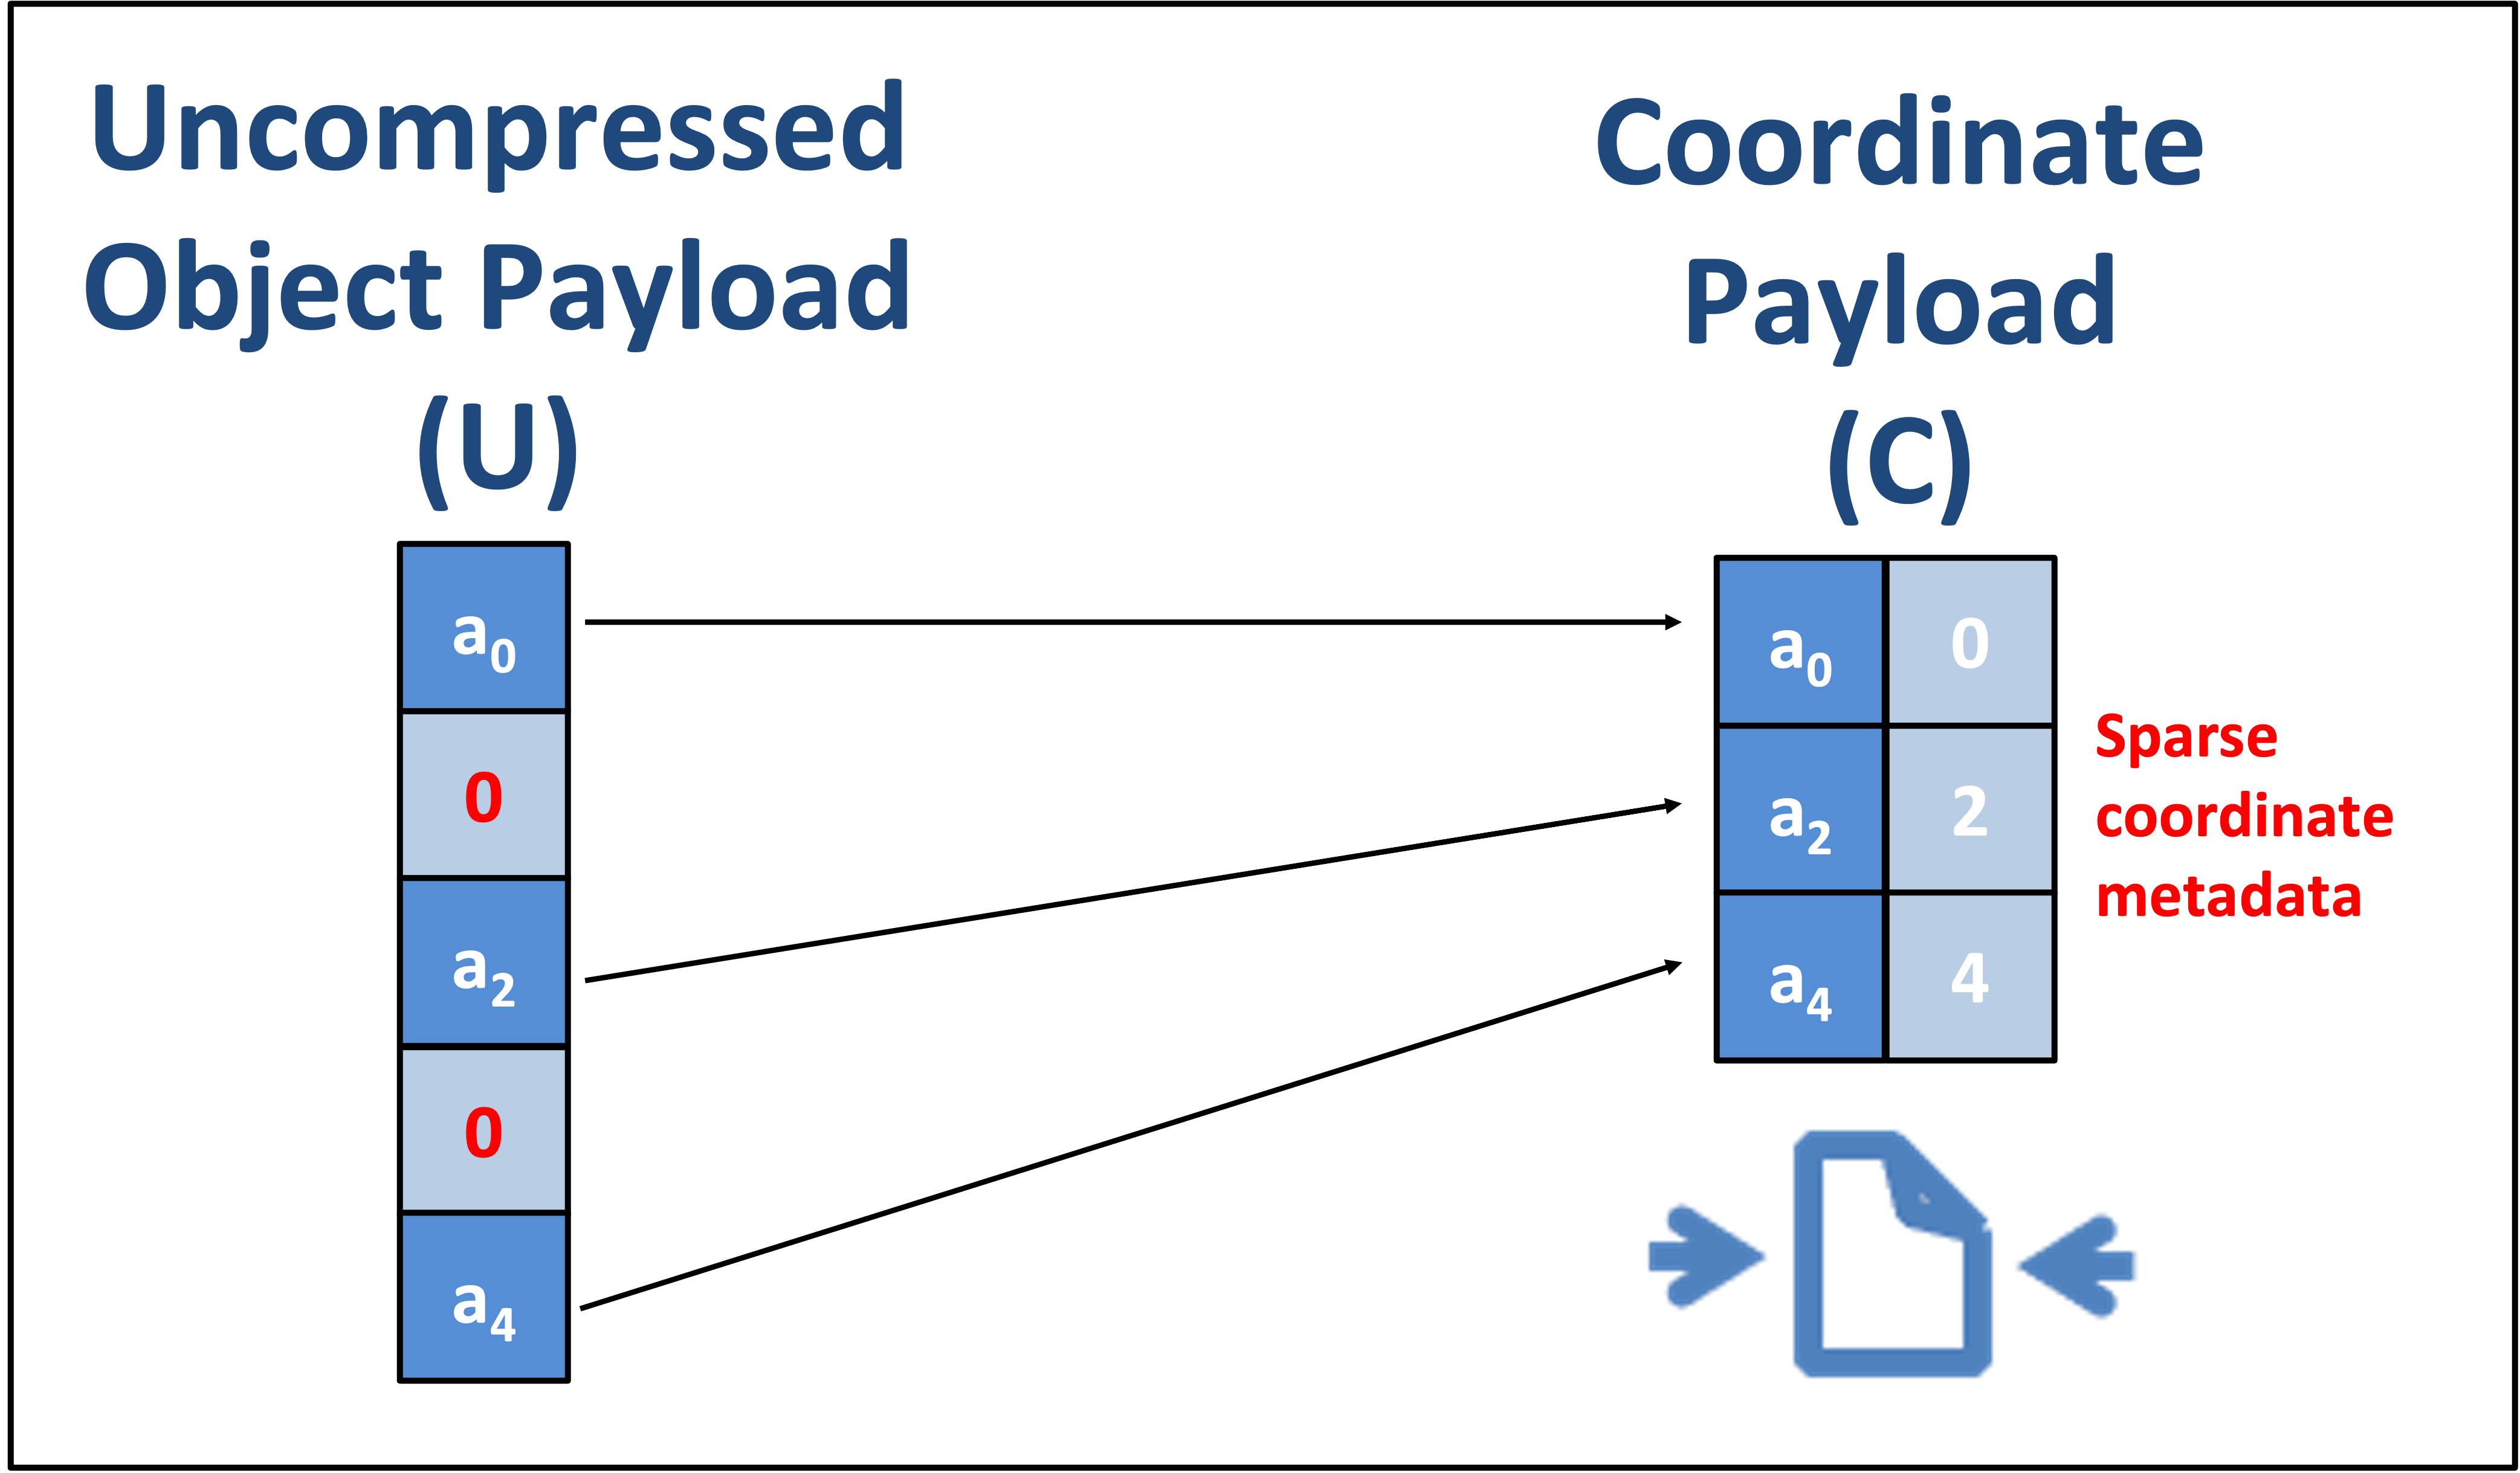
\includegraphics[width=8cm]{figures/saf_format_optimizations.PNG}
\caption{A visualization of a compressed representation format (coordinate-payload or CP) applied to a vector with some zero entries. The compressed representation is reduced to nonzero values and metadata which recovers the original data structure.}
\label{fig:saf_format_optimizations}
\end{figure}
%
% Content: format optimizations
%

%
% Figure: combined action/format optimizations
%
\begin{figure}[h]
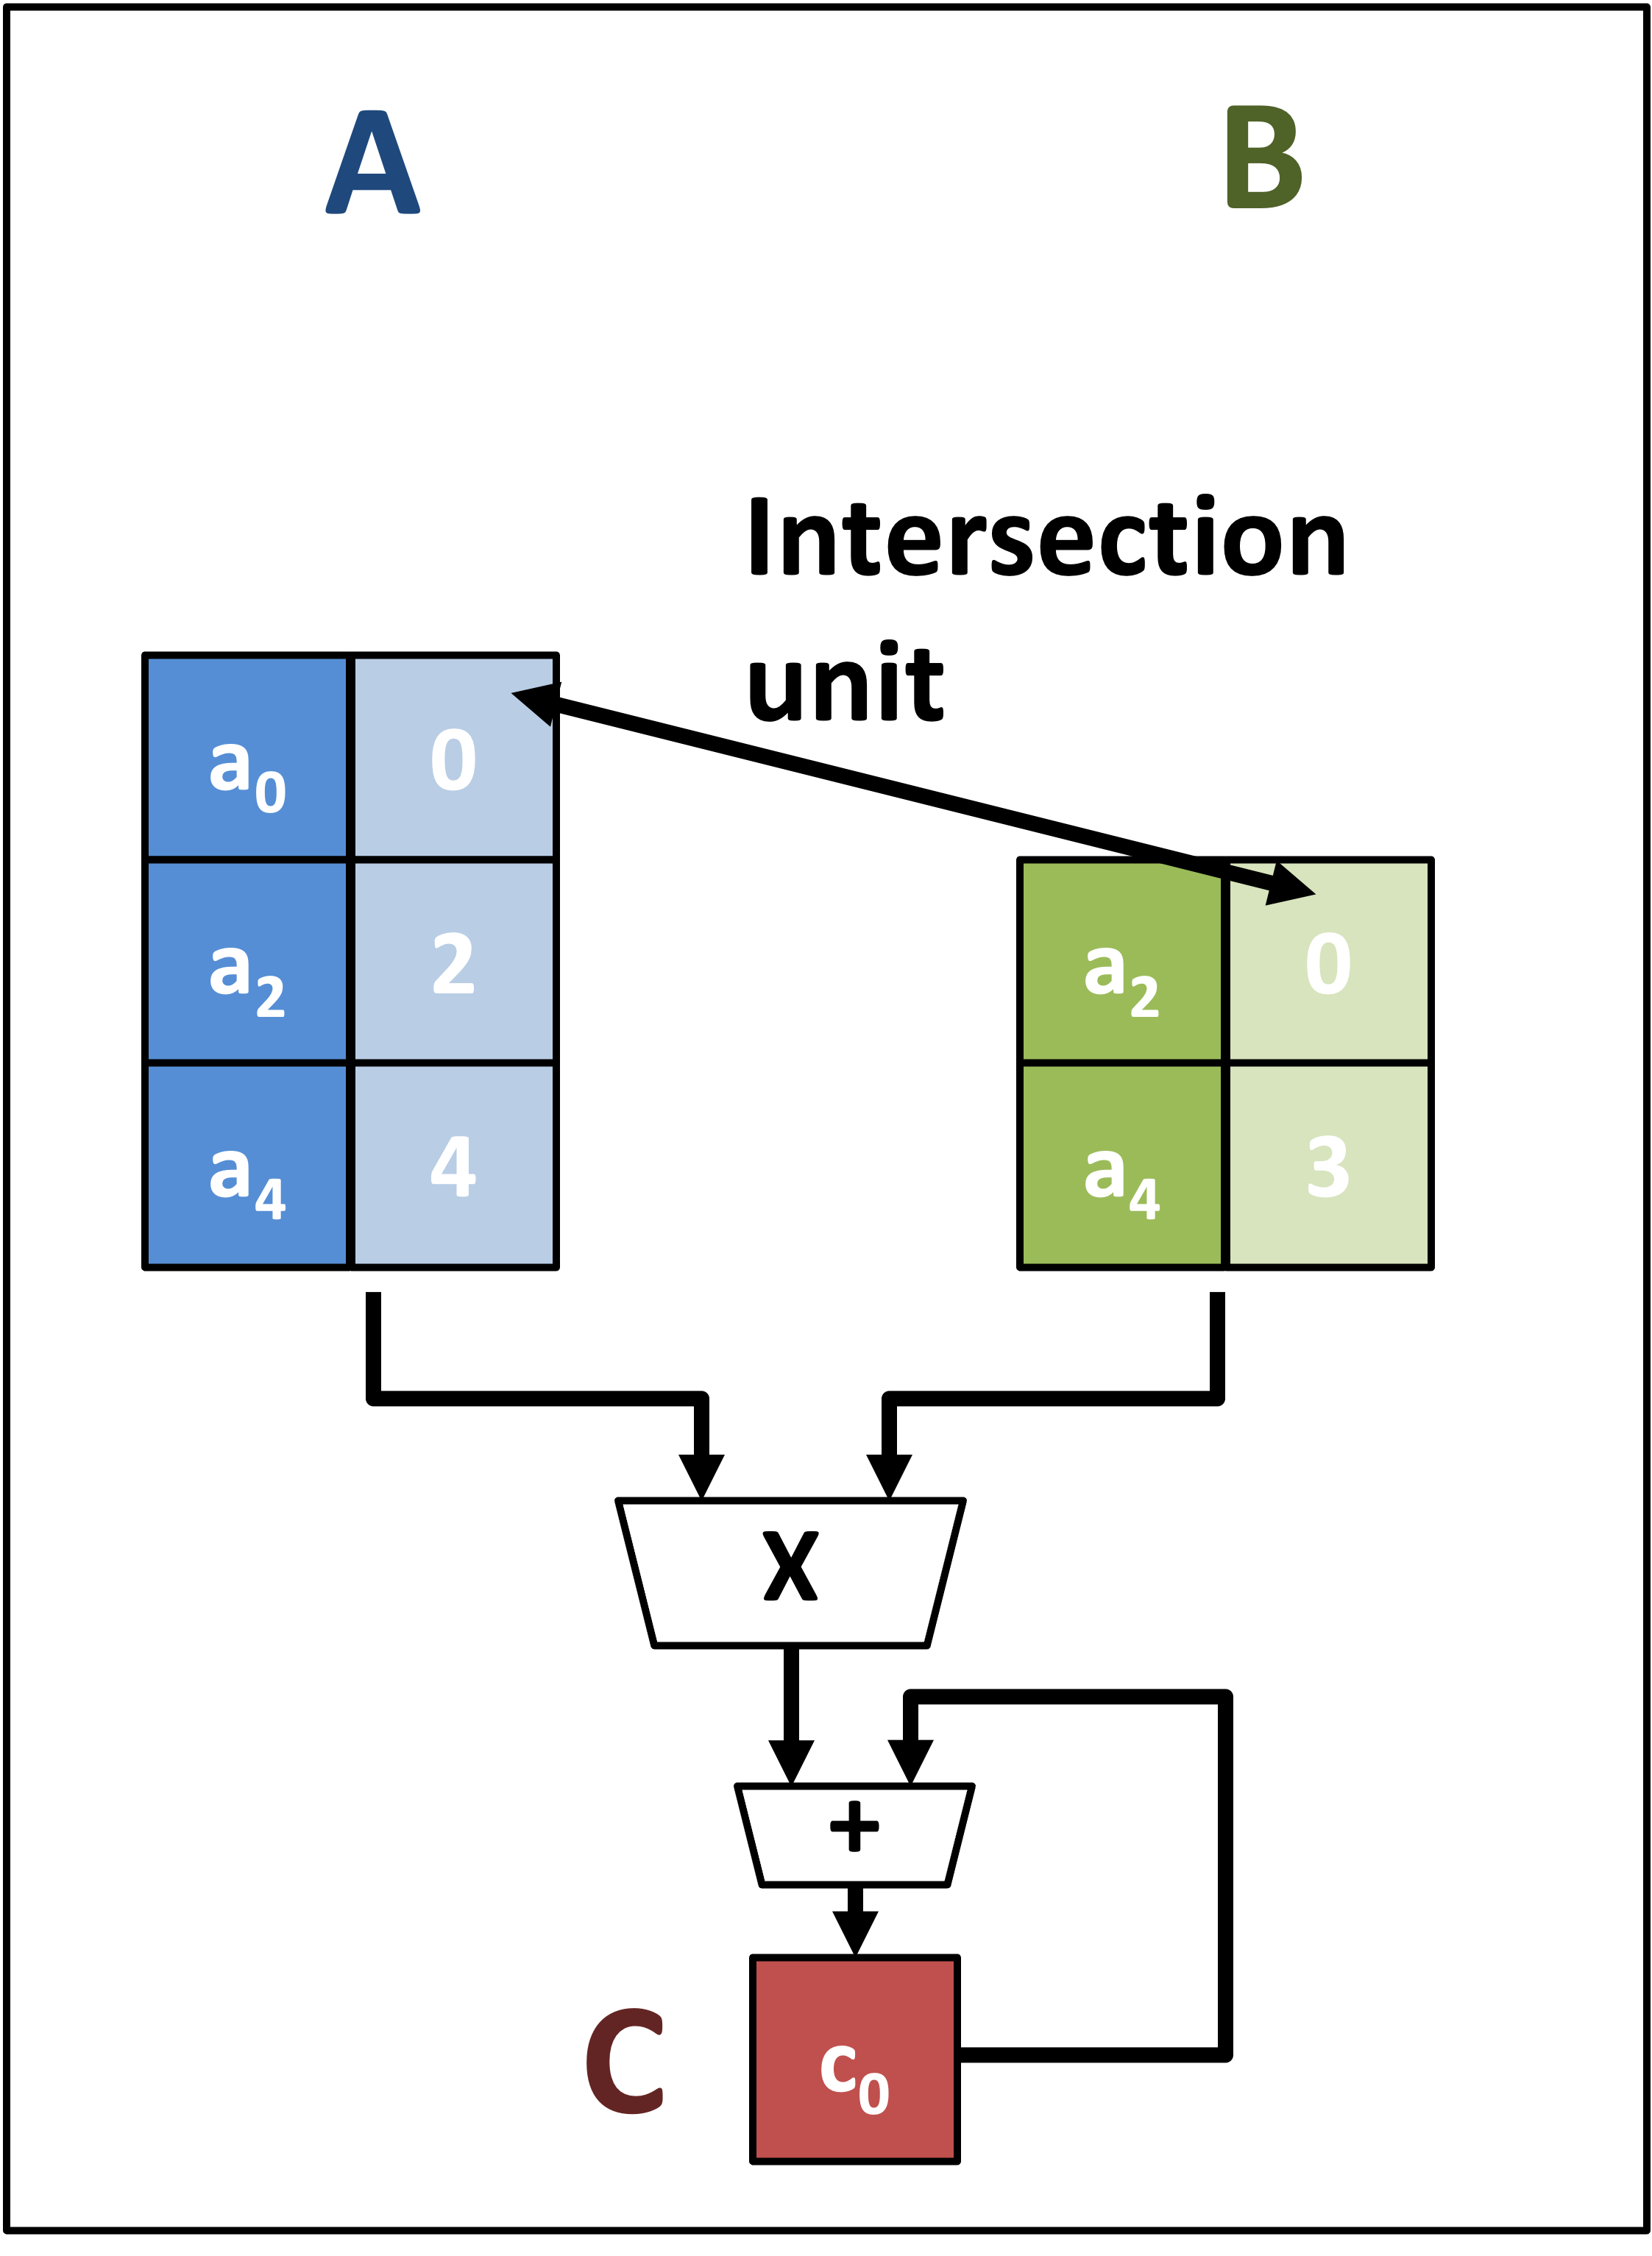
\includegraphics[width=4cm]{figures/saf_action_format_combo.PNG}
\caption{An example of dot-product optimized with both bidirectional zero-skipping and a compressed representation format. Conceptually corresponding nonzero values must be matched using a component which processes format metadata in order to implement skipping, which is called an \textit{intersection unit.} The cost of the skipping optimization is the energy, area and latency of the skipping microarchitecture, which comprises the intersection unit.}
\label{fig:saf_action_format_combo}
\centering
\end{figure}
%
% Figure: architecture example
%
\begin{figure}[h]
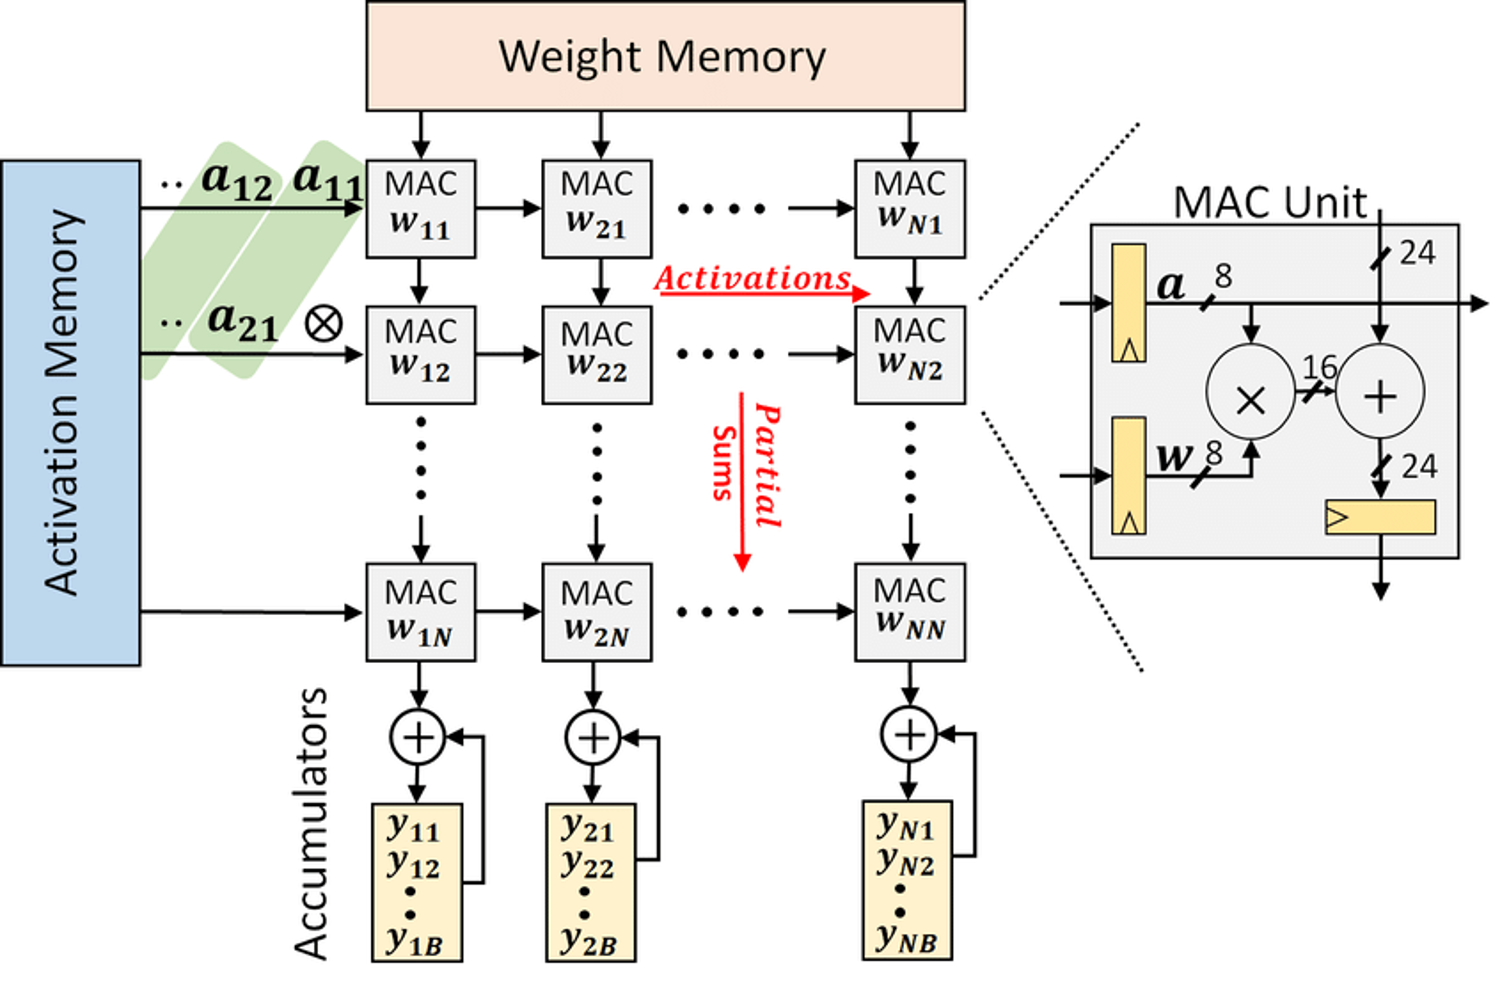
\includegraphics[width=8cm]{figures/arch_example.PNG}
\caption{A tensor accelerator \textit{architecture} (Thunderbolt architecture, figure from \cite{examplearch}.)}
\label{fig:saf_format_optimizations}
\end{figure}
%
% Figure: microarchitecture example
%
\begin{figure}[h]
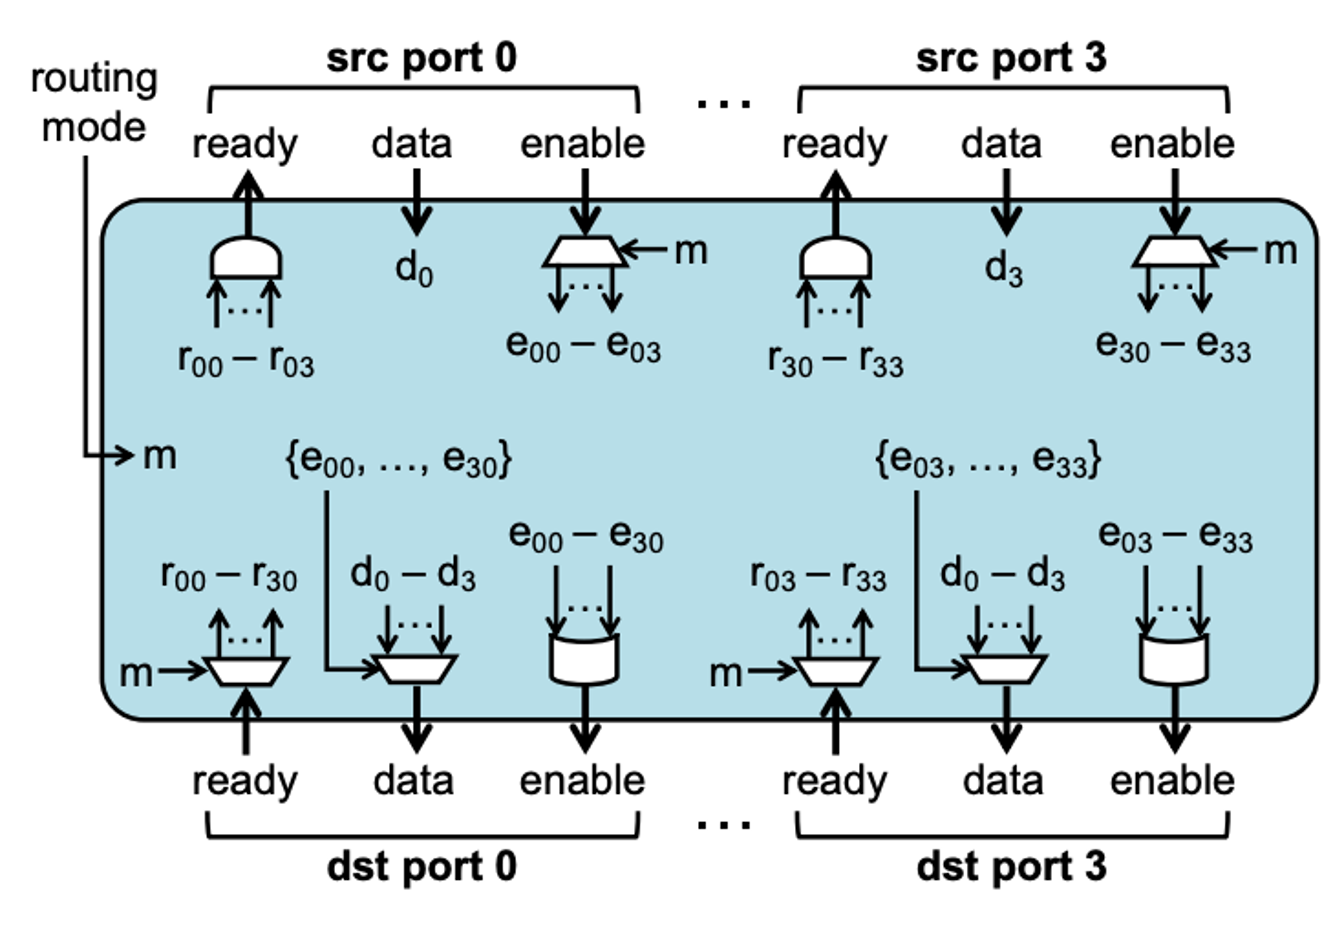
\includegraphics[width=8cm]{figures/uarch_example.PNG}
\caption{Tensor accelerator \textit{microarchitecture} (Eyeriss v2 NoC switch, figure from \cite{eyerissv2}.)}
\label{fig:saf_format_optimizations}
\end{figure}
%
% Figure: SAFs can be significant or not, it depends on the microarchitecture
%
\begin{figure*}[ht]
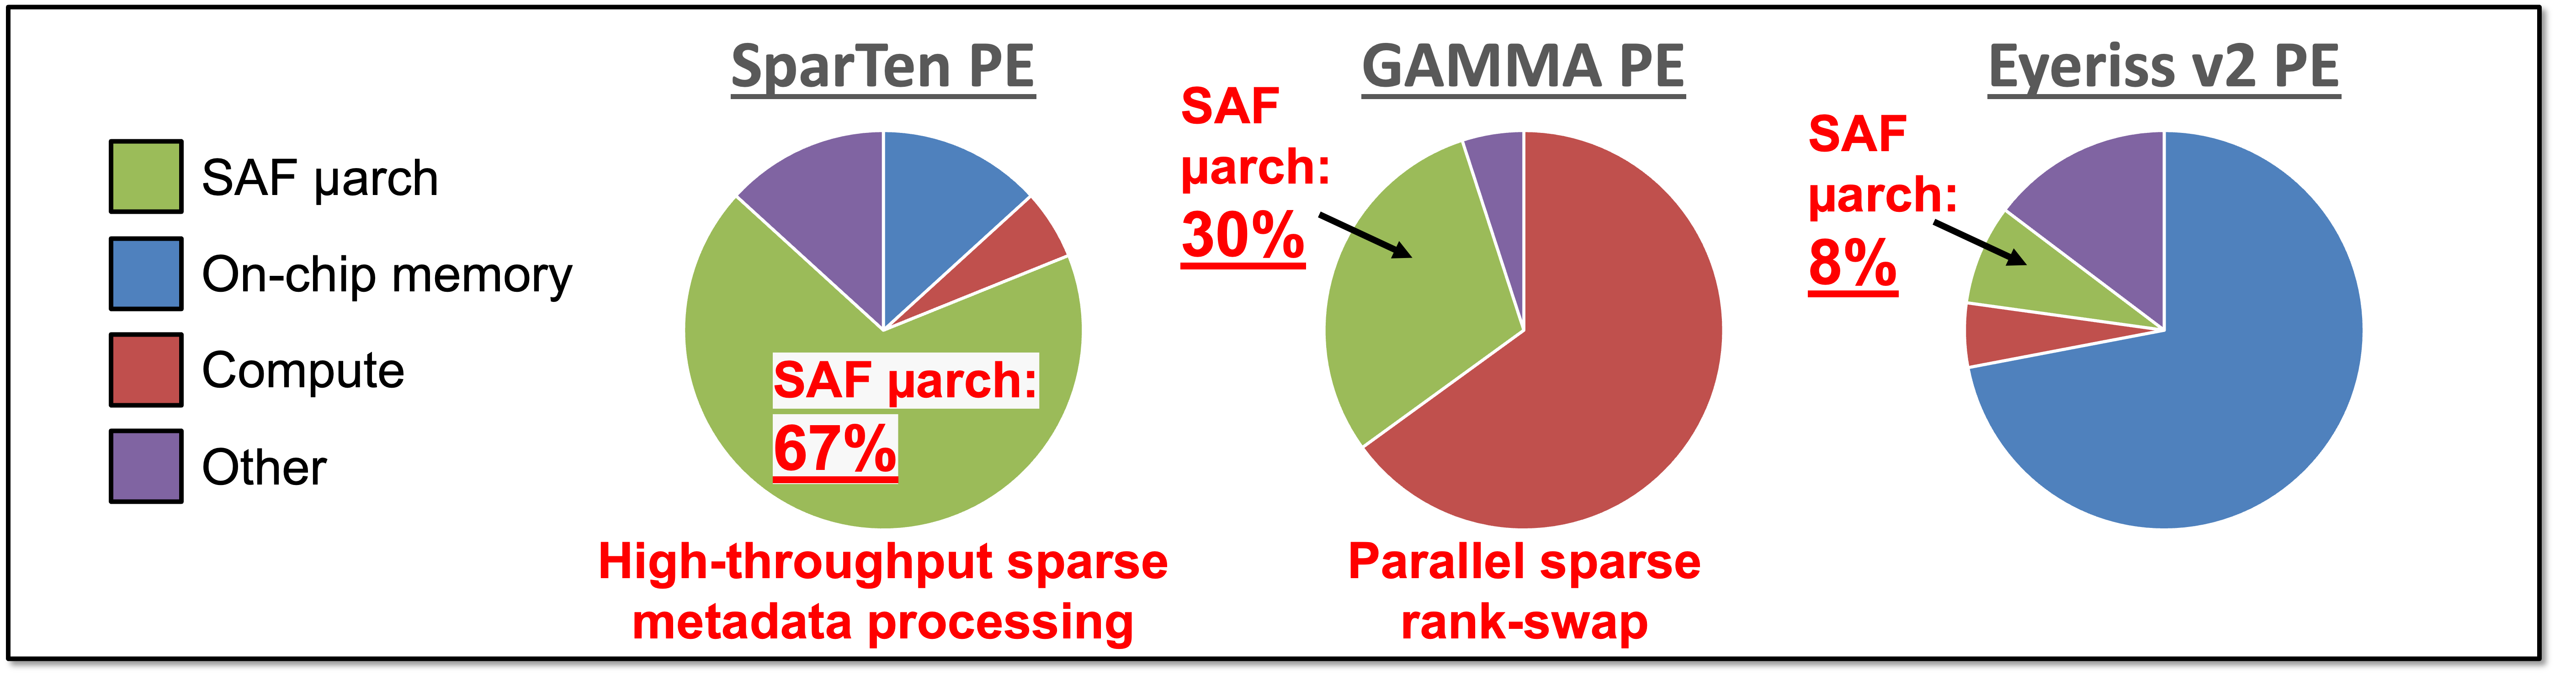
\includegraphics[width=\textwidth]{figures/saf_uarch_significance.PNG}
\caption{Breakdown of sparse tensor accelerator PE area based on published RTL simulations for a representative sample of designs. The total area of PE architectural components is a decent model of Eyeriss v2\cite{eyerissv2} PE area because Eyeriss v2's simple leader-follower zero-skipping microarchitecture has negligible area. SparTen\cite{sparten} employs a complex zero-skipping microarchitecture which must process high-throughput bitmask metadata. GAMMA's\cite{gamma} PE coordinates loop-nest re-ordering with tensor layout shuffling while the data is in-flight, using a high-radix merger component. These complex microarchitectures create discrepancies against architectural PE models.}
\label{fig:saf_uarch_significance}
\centering
\end{figure*}
%
% Figure: prior work
%
\begin{table*}[ht]
\begin{tabular}{c|c|}
\textbf{Accelerator} & \textbf{SAF microarchitecture proposals} \\ \hline \hline
Eyeriss &  MAC gating; in-flight RLE decompression \\ \hline
Eyeriss v2 & CSC zero-skipping \\ \hline
ExTensor & Hierarchical bidirectional zero-skipping \\ \hline
SCNN & Memory conflict handling (binning output coordinates) \\ \hline
SparTen & Bitmask zero-skipping, parallel compression, memory conflict handling \\ \hline
OuterSPACE & Software rank-swap \\ \hline
GAMMA & Leader-following intersection, hardware rank-swap \\ \hline
\end{tabular}
\caption{A non-exhaustive list of published tensor accelerators and their proposed SAF microarchitectures.}
\label{tab:design_specific_models}
\centering
\end{table*}

\section{SAF microarchitectures}

Prior research on sparse tensor acclerators proposes many different SAF microarchitectures, without employing a consistent set of abstractions and models in order to explore the design space or make comparisons. However, the breakdown of PE area for several accelerator designs in Figure~\ref{fig:saf_uarch_significance} shows that it is not always safe to assume SAF microarchitecture overhead is insignificant, and so it is important to choose SAFs and SAF microarchitecture designs systematically to minimize cost.

The Eyeriss v2\cite{eyerissv2} PE implements a leader-follower skipping SAF, devoting only 8\% of its PE area to the skipping microarchitecture. This is owing to a lightweight leader-follower skipping microarchitecture which operates on sparse weights and activations in Compressed-Sparse Column (CSC) format. 

In contrast, the SparTen\cite{sparten} accelerator PE uses most of its PE area for the bidirectional skipping microarchitecture which operates on Bitmask-format metadata. As will be shown later, this is attributable to the substantial load-handling capability which the skipping microarchitecture must have in order to maintain high arithmetic hardware utilization. 

As a final example, the GAMMA\cite{gamma} accelerator PE devotes 30\% of its PE area - a significant amount - in order to apply a rank swap\footnote{Here, rank swap is used to refer to transposition of the traversal-order of tensor ranks, as described in\cite{TODO}.}. The PE employs a row-wise product dataflow for loading CSR-format GEMM ($C_{M\times N} = A_{M\times K} \times B_{K\times N}$) operands from memory. A single $A_{M\times K}$ element and a row of $B_{K\times N}$ elements are loaded from on-chip memory into the PE; this reflects that the $N$ rank of B is traversed in the inner-most loop, while the contracted $K$ rank is traversed at an intermediate loop level. Row-wise product enables a cheap leader-follower skipping microarchitecture to be employed for loading $B_{K\times N}$ rows conditional on non-zero $A_{M\times K}$ elements. Upon receiving $A_{M\times K}$ and $B_{K\times N}$ values from memory, the GAMMA PE implements a rank-swap which moves the contracted dimension $K$ into the innermost loop. This enables inner-product accumulation into a single PE output register. The output memory footprint saved by the rank-swap is significant: a design such as MatRaptor\cite{matraptor} which implements row-wise product \textit{without} a rank-swap must store and incrementally accumulate $|K|$ rows of partial outputs, each of size $1 \times |N|$, requiring increased output memory footprint. Given the benefit of rank-swap, is there a tradeoff involved in using it? The use of CSR in GAMMA, means thank rank-swap requires a merge primitive (analogous to the merge operation in mergesort) in order to sort $B_{K\times N}$ operand data first by $K$ coordinate metadata, and then by $N$ coordinate metadata, effectively implementing a transpose. GAMMA employs a radix-64 merge unit\cite{gamma} in order to do this. Although the rank-swap itself is not a sparse optimization, nonetheless the need for this type of merge unit results from employing a rank-swapped dataflow \textit{in the context of employing CSR format for the $B_{K\times N}$ operand}. Thus it is justifiable to say that the merge unit is part of the format microarchitecture which implements the CSR format SAF. It is this format microarchitecture which accounts for 30\% of PE area in GAMMA.

Clearly, SAFs and SAF microarchitecture designs are complex and impactful design decisions, and it is desirable to know whether a particular combination of SAFs will lead to the substantial PE implementation overhead seen (for example) in SparTen and GAMMA. The rest of this work develops a conceptual framework for taxonomy and modeling of SAF microarchitectures. This conceptual framework can be represented in software and utilized for make SAF microarchitecture design decisions using analytical pre-RTL modeling tools.

%\subsection{Smartbuffer model and Format microarchitecture}
%\subsubsection{Dense smartbuffer}
%\subsubsection{Sparse smartbuffer}
%\subsubsection{Format interfaces}

\label{background:saf_uarch}
\chapter{SAF microarchitecture design space}

This section summarizes key design choices which form the SAF microarchitecture design space.

\section{SAF attributes}
%
% Figure: SAF attributes impact uarch cost
%
\begin{figure*}[ht]
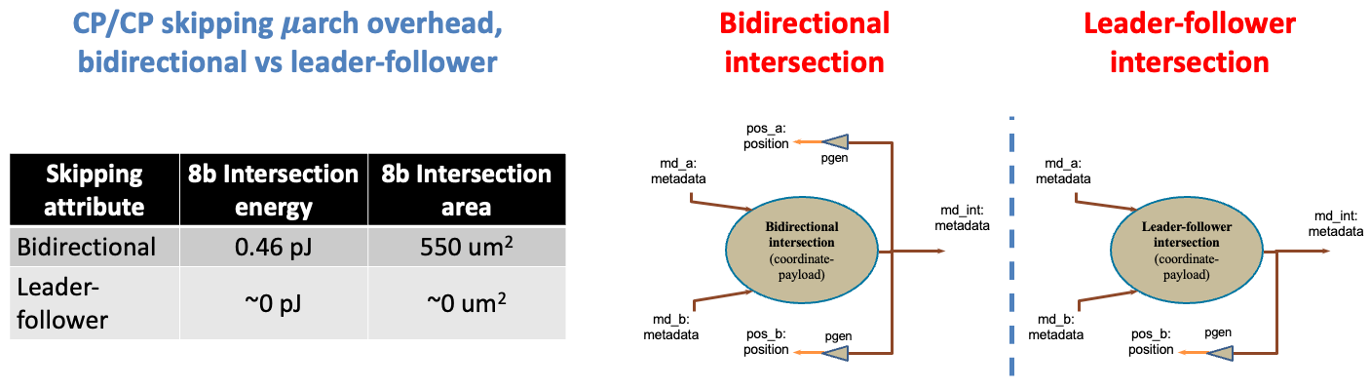
\includegraphics[width=\textwidth]{figures/saf_attributes_impact_uarch_cost.PNG}
\caption{Zero-skipping microarchitecture cost-comparison between an architecture with a bidirectional skipping SAF (left) and an architecture with a leader-follower skipping SAF (right.) Both architectures also employ a coordinate-payload format SAF.}
\label{fig:saf_attributes_impact_uarch_cost}
\centering
\end{figure*}
%
% Content: SAF attributes impact SAF microarchitecture cost
%
The attributes of a SAF impact the energy, area and latency of its SAF microarchitecture by implicitly constraining aspects of the design-space.
%
\subsection{SAF microarchitecture topology and primitive cost} 

Figure \ref{fig:saf_attributes_impact_uarch_cost} shows that a skipping SAF with the leader-follower attribute can have an implementation based on simple control logic that conditions MACs and follower reads on whether there is a nonzero leader operand. The energy and area overhead to implement this SAF is low. However designers may choose bidirectional skipping SAF instead in order to skip 100\% of ineffectual operations; this results in more expensive skipping microarchitecture with comparison logic to detect either or both zero operands, incurring a significant energy and area overhead. Generally, simple changes in the SAF optimization strategy may (or may not) have dramatic impact on microarchitecture complexity and thus on energy, area and latency.
%
\subsection{SAF primitive design}
%
\todo{Don't use terminology (i.e. primitive) which is not yet introduced.}
%
\section{Load-handling requirements}
%
\section{Optimizations}

\subsection{Algorithm}

\subsection{Pipelining}
%
\section{Cross-architecture impacts}


\chapter{SAF microarchitecture taxonomy}

In this work, SAF microarchitecture categorization is intended to facilitate communication of general design principles, very early planning discussions among designers, and design-space exploration of possible SAF microarchitectures. \todo{It is important to set up a systematic way of describing components and how they connect to each other. Later, we use this taxonomy as the basis of a set of tools for inferring the SAF microarchitecture design and modeling its energy, area and latency.} \\
%
A sufficiently expressive taxonomic framework encompasses SAF microarchitecture designs seen in the literature and may also express design not yet developed, enabling improvements on existing work. However a highly detailed and expressive representation of microarchitecture as, i.e., RTL, is not ideal because the design-space is huge and difficult to describe or constrain, or even to extract general design principles from. Existing architectural modeling tools face similar problems with exponential growth in the space of possible designs as the language for describing designs becomes more expressive, which they address by (1) limiting to a finite set of architectural primitives (i.e. SRAM, MAC, etc.)\cite{timeloop}, (2) supporting hierarchical component representations built out of primitives \cite{accelergy} such that a small primitive library enables a large space of designs, (3) parameterizing component categories with a concise set of attributes that are sufficient to narrow down an implementation \cite{accelergy}, (4) describing optimizations (i.e. SAFs as described in \cite{sparseloop}) as annotations on architectural components which themselves have attributes sufficient to describe the optimization strategy, and (5) producing frameworks which are extensible to help designers to concisely express key design-specific components. \todo{Antipattern - paper on specific microarchitectures only.} \\
%
This work addresses the challenge of describing SAF microarchitectures in an expressive but concise way, which is easily extensible by users. Ideally a designer could express many useful SAF microarchitectures as a netlist or schematic, not of logic gates, but of connections between higher-level ``SAF primitive components'' which recur frequently across published SAF microarchitecture designs. Components are further parameterized with attributes sufficient to narrow down the general energy, area and latency scaling behavior of the underlying implementation. To that end, the conceptual framework developed in this work consists of
%
\begin{itemize}
    \item A taxonomic categorization of SAF primitives
    \item For each taxonomic primitive, a set of attributes sufficient to narrow down the general type of microarchitecture implementation as well as the scaling behavior of energy, area and latency
    \item For each SAF described in \cite{sparseloop} (format, gating, skipping), a feasible set possible topologies for building the SAF microarchitecture out of SAF primitives
    \item For each SAF, a set of attributes which are sufficient to narrow down the appropriate SAF microarchitecture out of the feasible set. This set includes at least the attributes of the SAF itself (i.e. type of action optimization, or choice of representation format), as well as other attributes specific to the SAF microarchitecture.
\end{itemize}

\section{Primitive components}

This section will overview the taxonomy of microarchitectural primitive components considered in this work.

\subsection{Metadata parsers}

\begin{figure}[H]
    \centering
    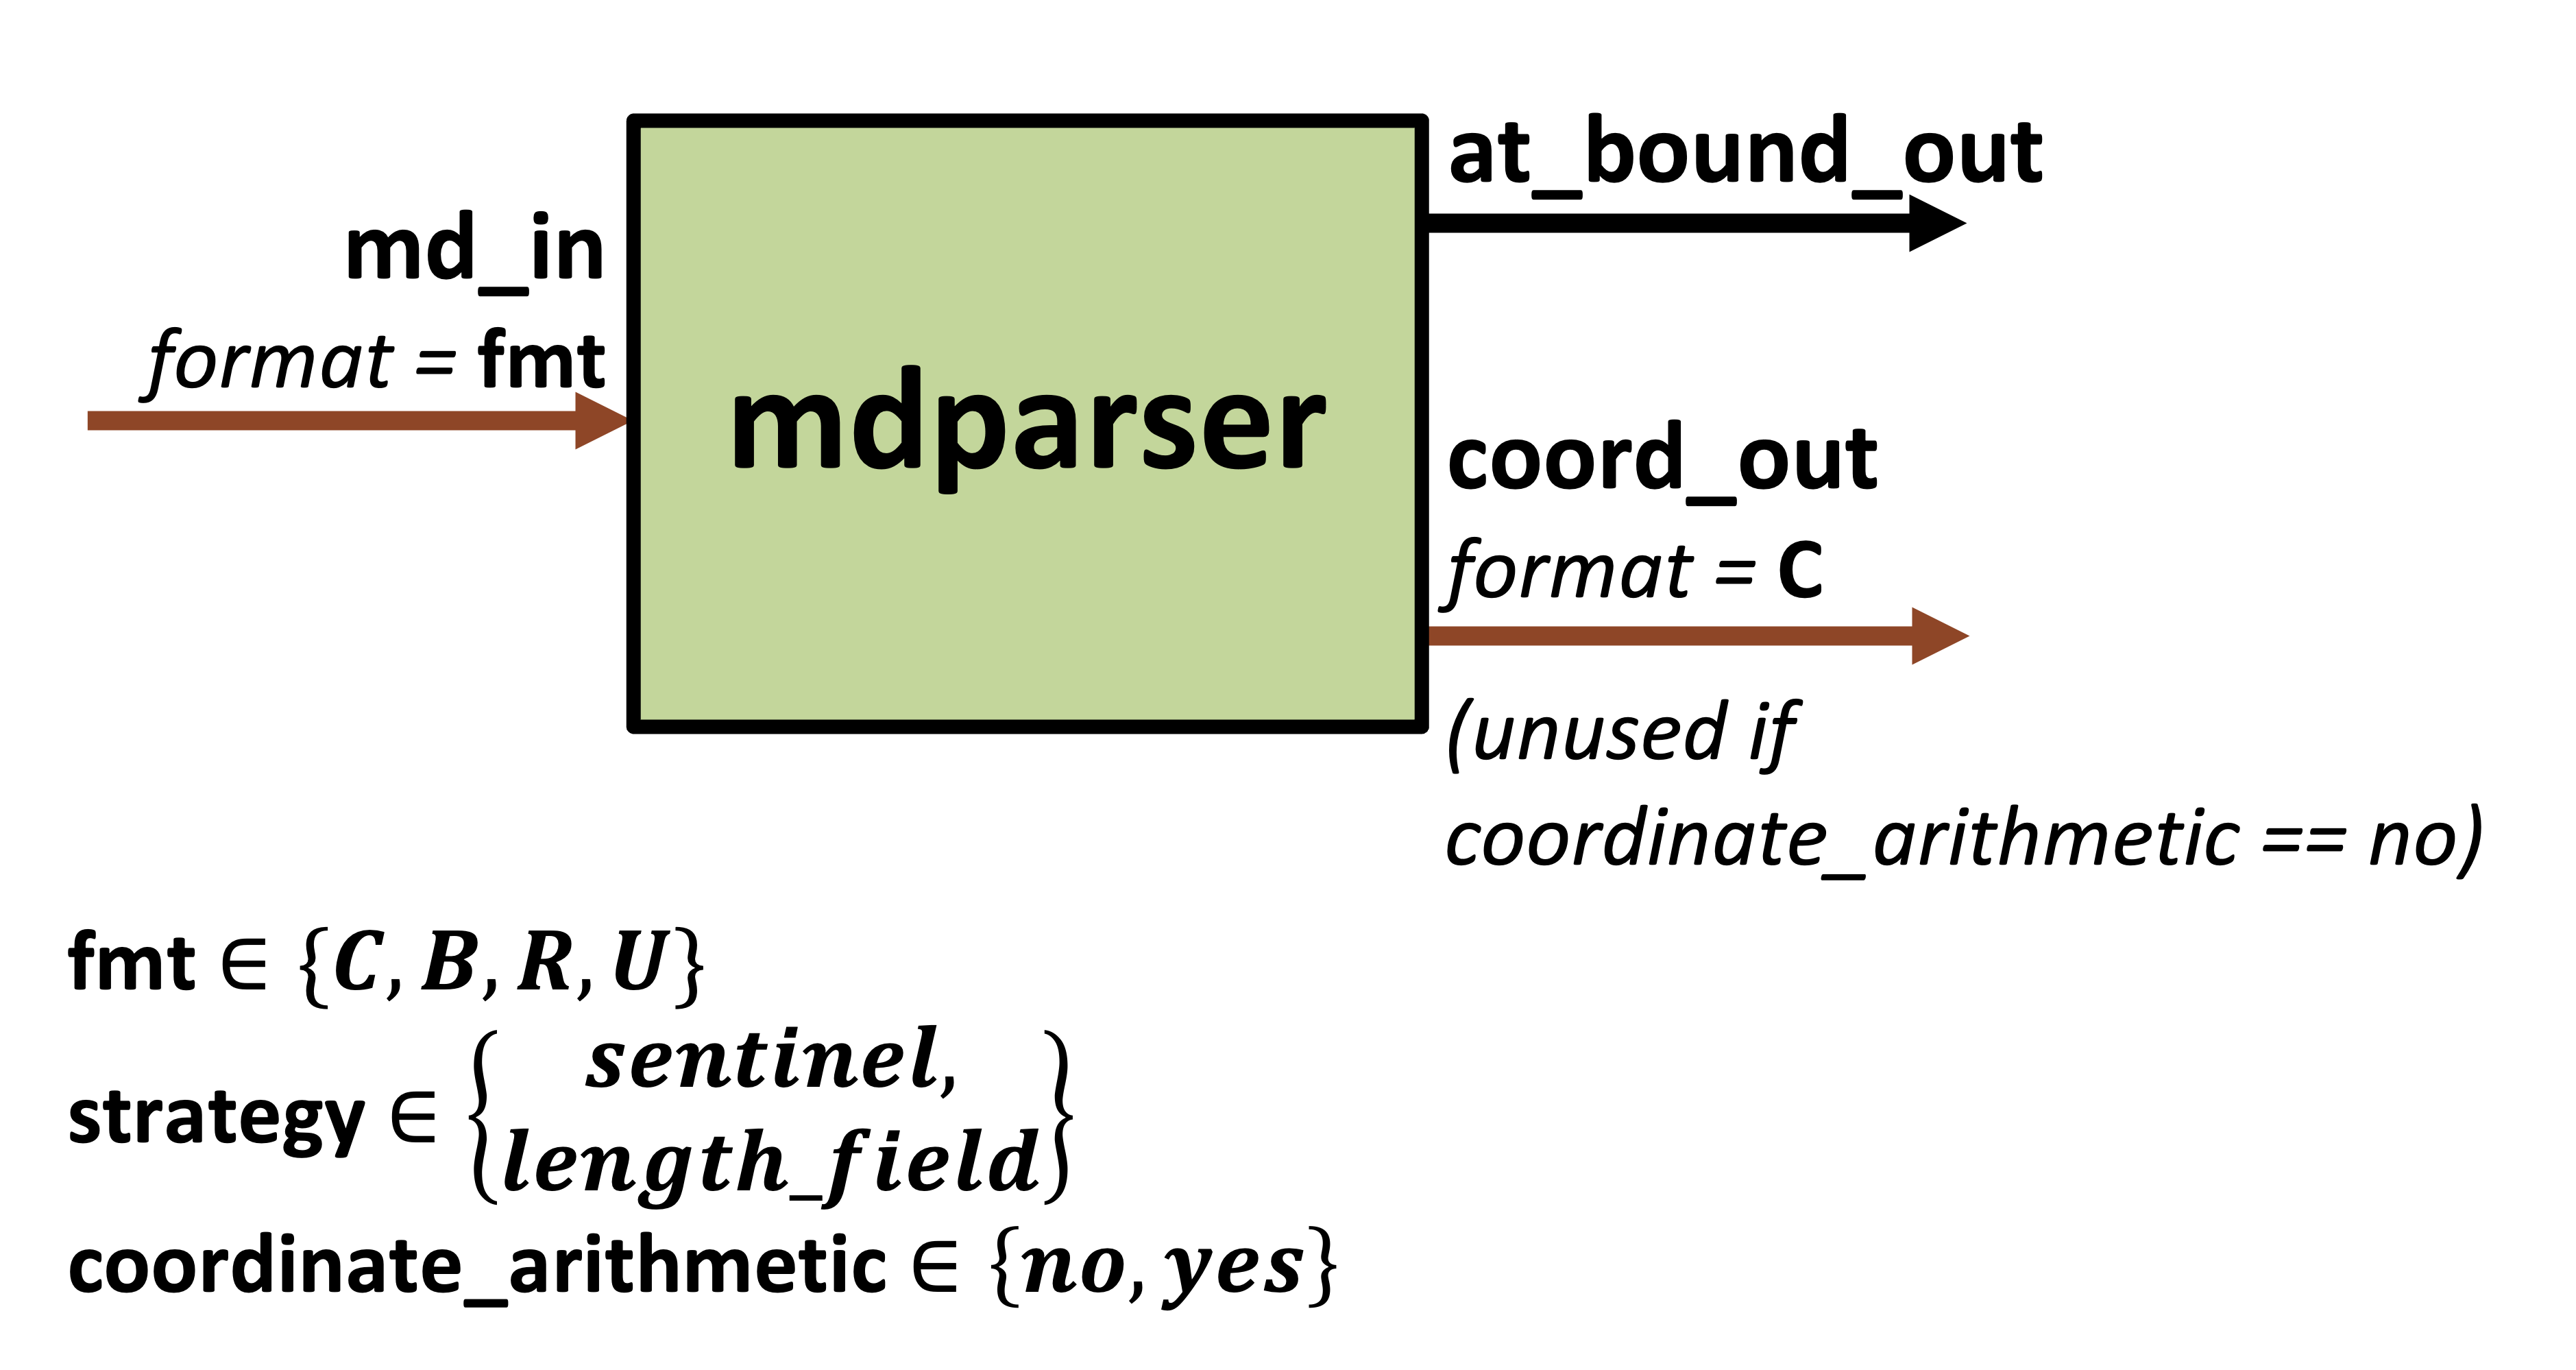
\includegraphics[width=0.95\textwidth]{figures/mdparser.png}
    \caption{Metadata parser primitive component template.}
    \label{fig:mdparser}
\end{figure}

\begin{table}[H]
\centering
\begin{tabular}{lll}
\toprule
 format   & strategy       & coordinate\_arithmetic   \\
\midrule
 U        & sentinel & no\_arithmetic                \\
 U        & sentinel & yes\_arithmetic                 \\
 U        & length\_field & no\_arithmetic              \\
 U        & length\_field & yes\_arithmetic             \\
 C        & sentinel & no\_arithmetic                \\
 C        & sentinel & yes\_arithmetic                 \\
 C        & length\_field & no\_arithmetic              \\
 C        & length\_field & yes\_arithmetic             \\
 B        & sentinel & no\_arithmetic                  \\
 B        & sentinel & yes\_arithmetic                 \\
 B        & length\_field & no\_arithmetic              \\
 B        & length\_field & yes\_arithmetic             \\
\bottomrule
\end{tabular}
\caption{Specializations of metadata parsers.}
\label{tab:MetadataParser_specializations}
\end{table}

\subsection{Position generators}

\subsubsection{Single position generators}

\begin{figure}[H]
    \centering
    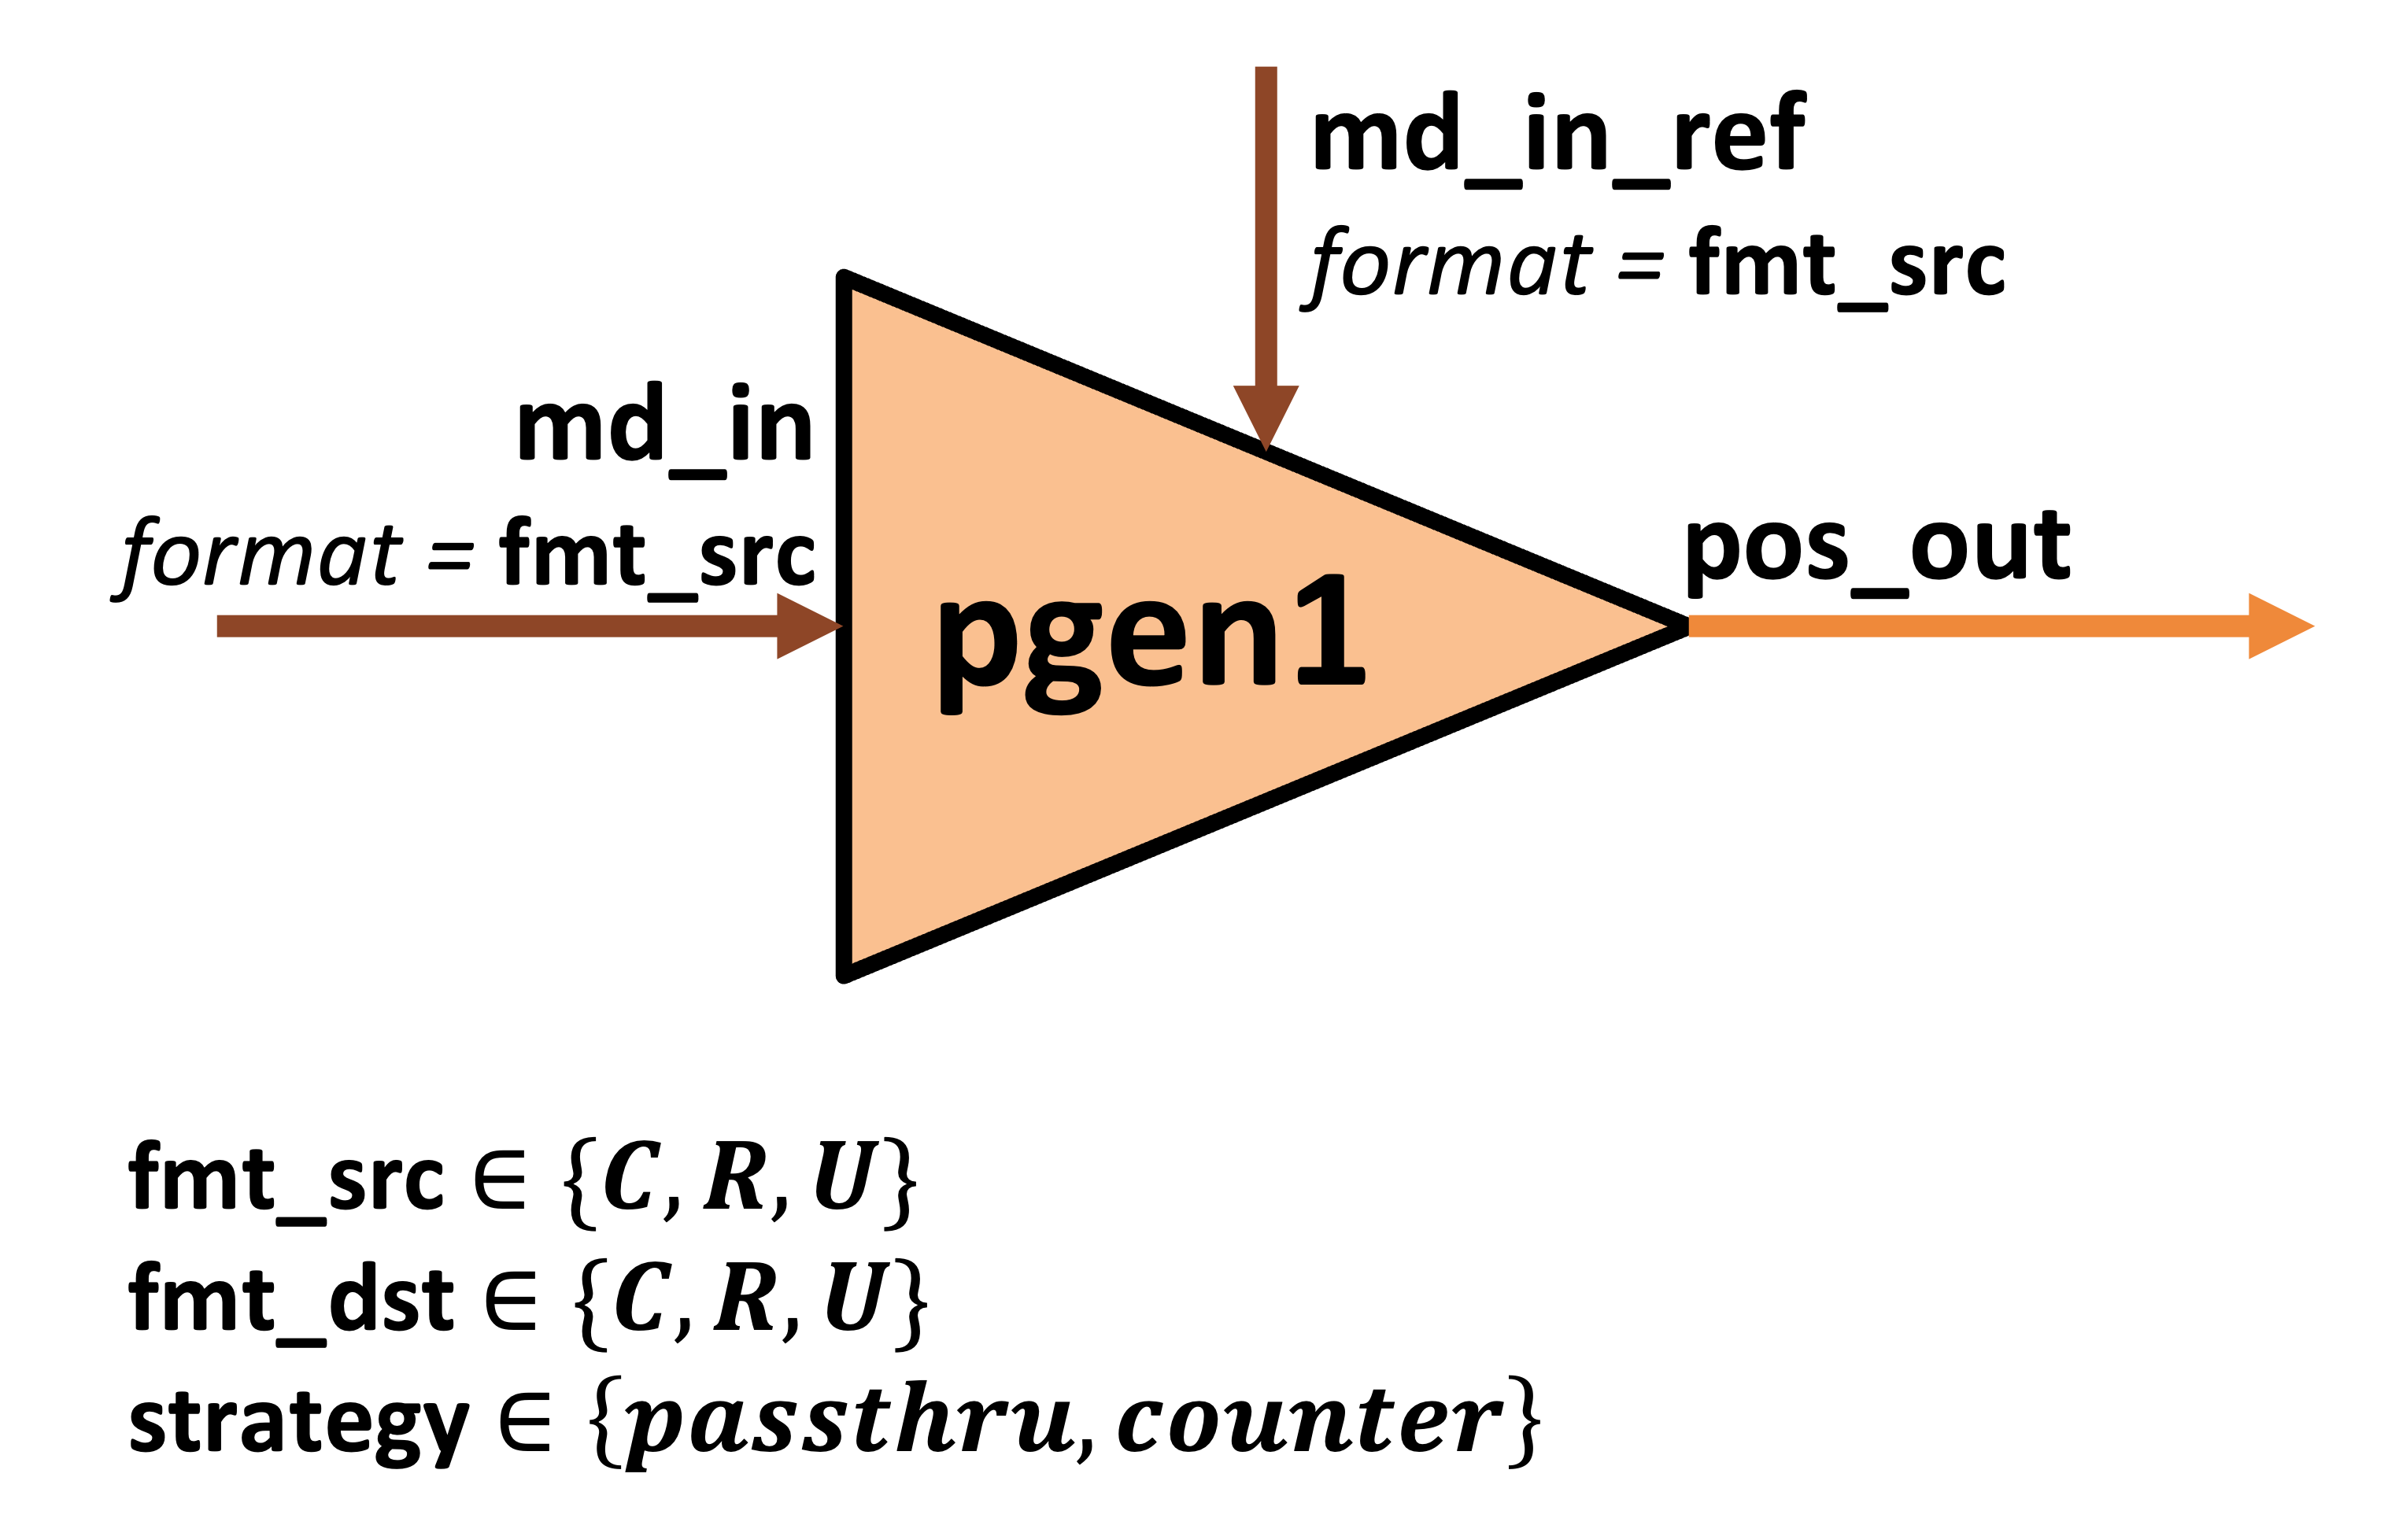
\includegraphics[width=0.95\textwidth]{figures/pgen1.png}
    \caption{Single position generator primitive component template.}
    \label{fig:pgen1}
\end{figure}

\begin{table}[H]
\centering
\begin{tabular}{lll}
\toprule
 format\_src   & format\_dst   & strategy    \\
\midrule
 C            & U            & passthrough \\
 C            & C            & counter     \\
\bottomrule
\end{tabular}
\caption{Specializations of single position-generator}
\label{tab:SinglePositionGenerator_specializations}
\end{table}

\subsubsection{Dual position generators}

\begin{figure}[H]
    \centering
    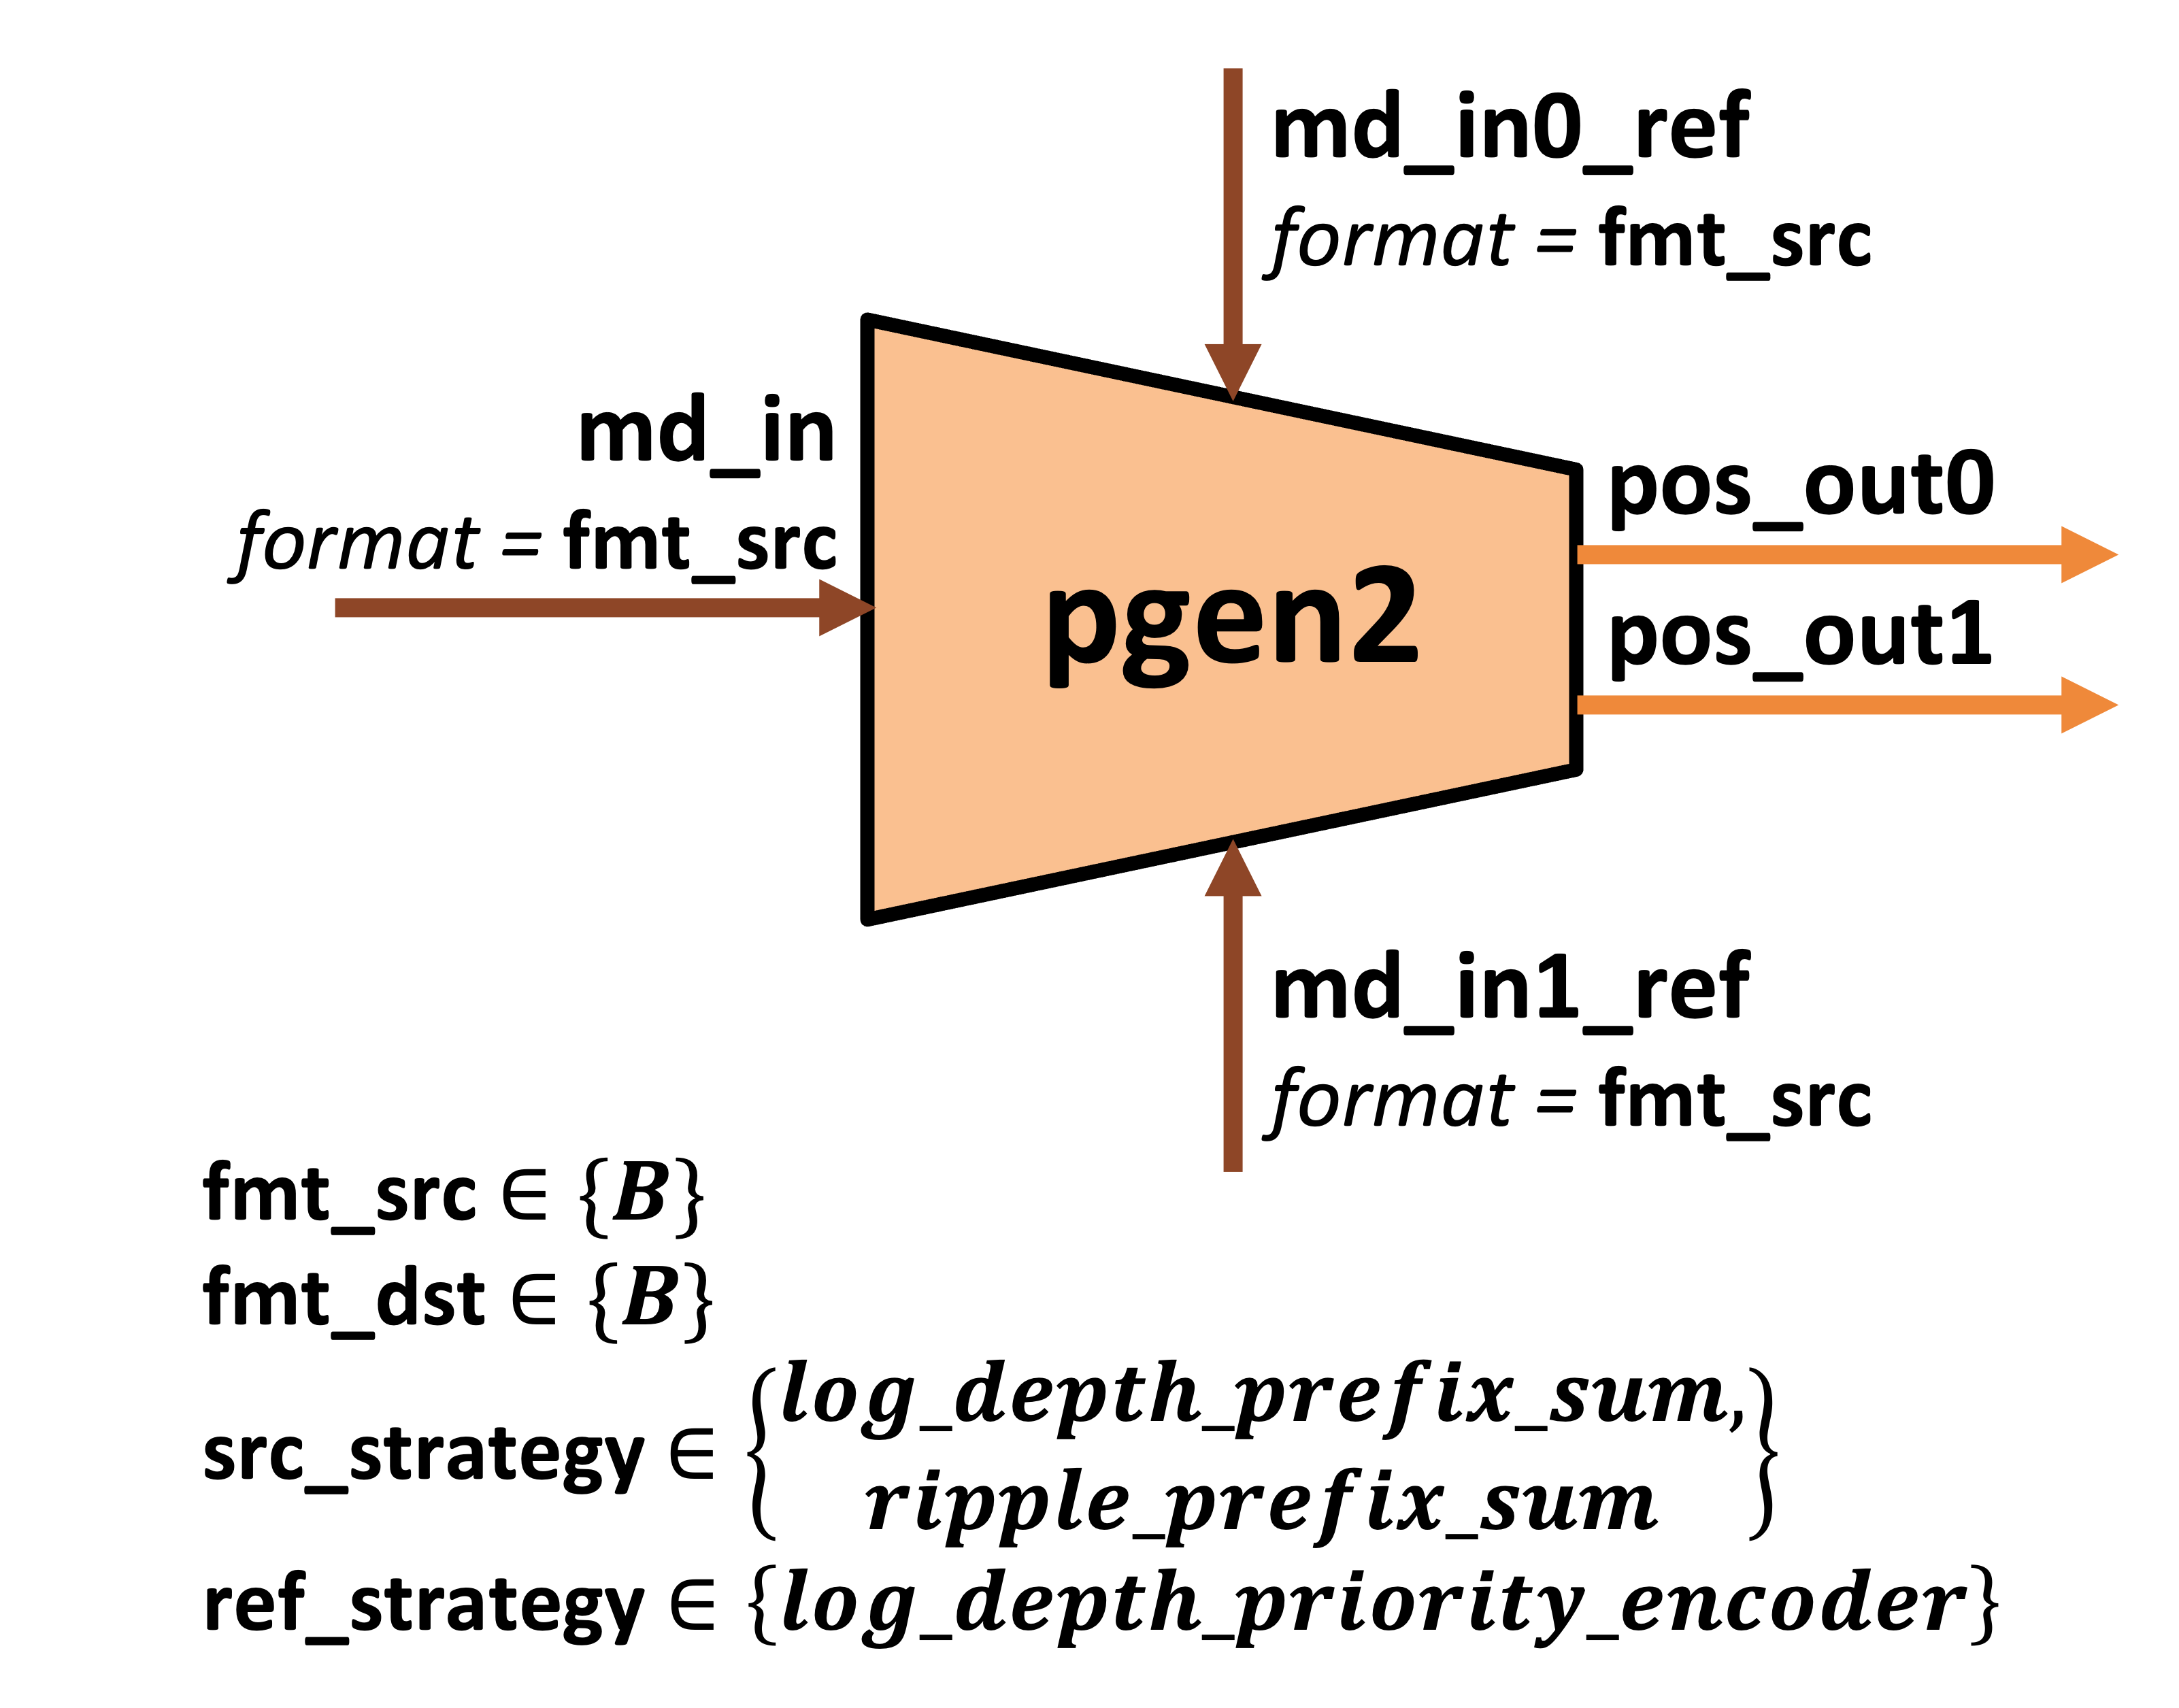
\includegraphics[width=0.95\textwidth]{figures/pgen2.png}
    \caption{Dual position generator primitive component template.}
    \label{fig:pgen2}
\end{figure}

\begin{table}[H]
\centering
\begin{tabular}{llll}
\toprule
 format\_src   & format\_dst   & source\_strategy        & reference\_strategy             \\
\midrule
 B            & B            & ripple\_prefix\_sum      & parallel\_dec2\_priority\_encoder \\
 B            & B            & kogge\_stone\_prefix\_sum & parallel\_dec2\_priority\_encoder \\
\bottomrule
\end{tabular}
\caption{Specializations of dual position generator}
\label{tab:DualPositionGenerator_specializations}
\end{table}

\subsection{Intersection units}

\subsubsection{Leader-follower intersection units}

\begin{figure}[H]
    \centering
    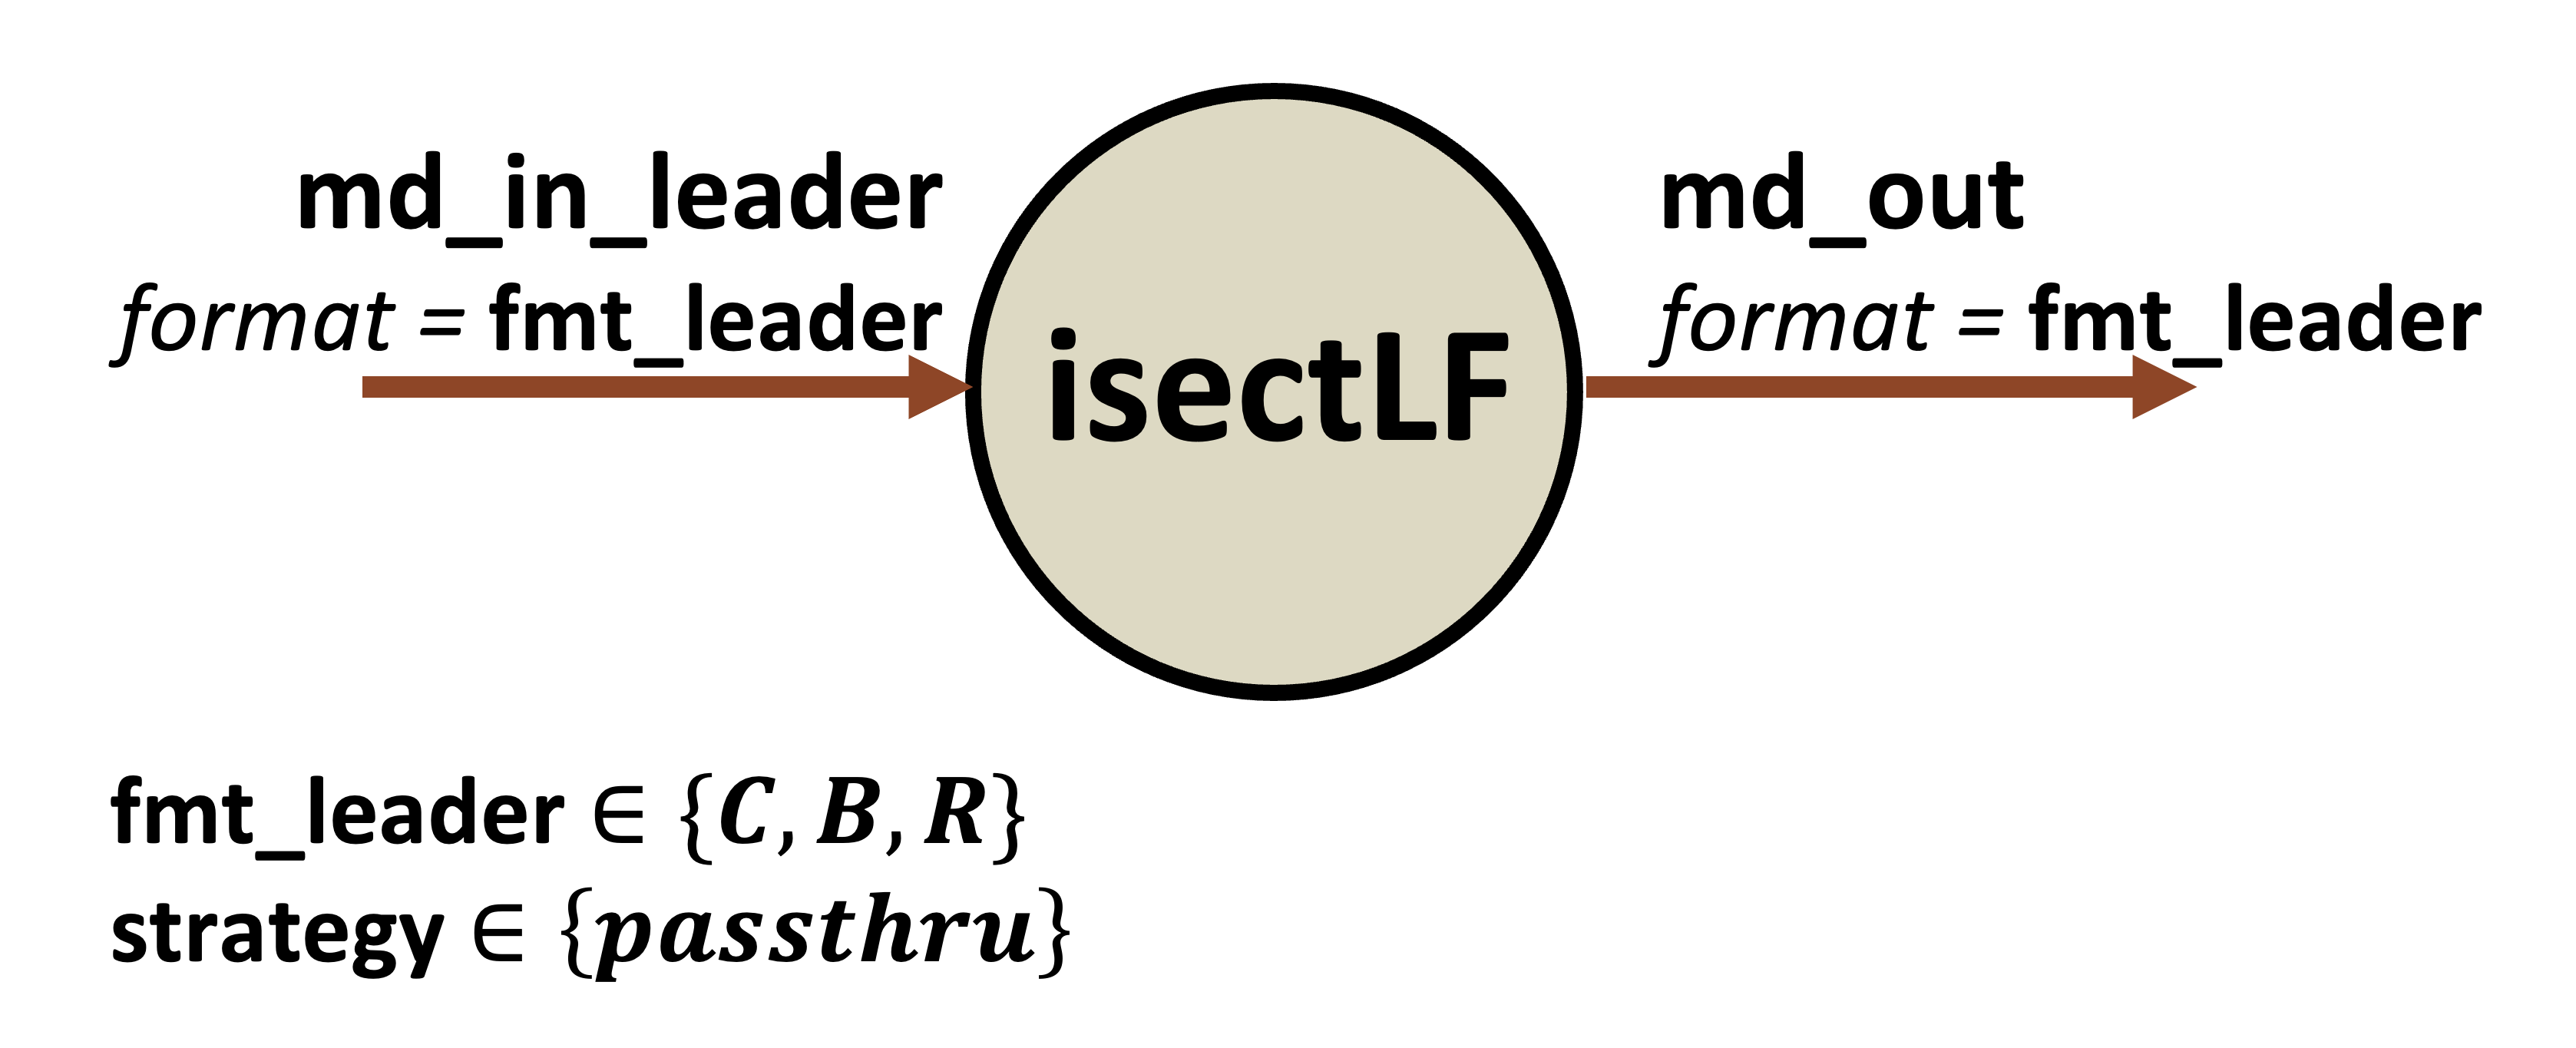
\includegraphics[width=0.95\textwidth]{figures/isectlf.png}
    \caption{Leader-follower intersection primitive component template.}
    \label{fig:isectlf}
\end{figure}

\begin{table}[H]
\centering
\begin{tabular}{ll}
\toprule
 format\_leader   & strategy    \\
\midrule
 C               & passthrough \\
 B               & passthrough \\
 R               & passthrough \\
\bottomrule
\end{tabular}
\caption{Specializations of leader-follower intersection.}
\label{tab:IntersectionLeaderFollower_specializations}
\end{table}

\subsubsection{Bidirectional intersection units}

\begin{figure}[H]
    \centering
    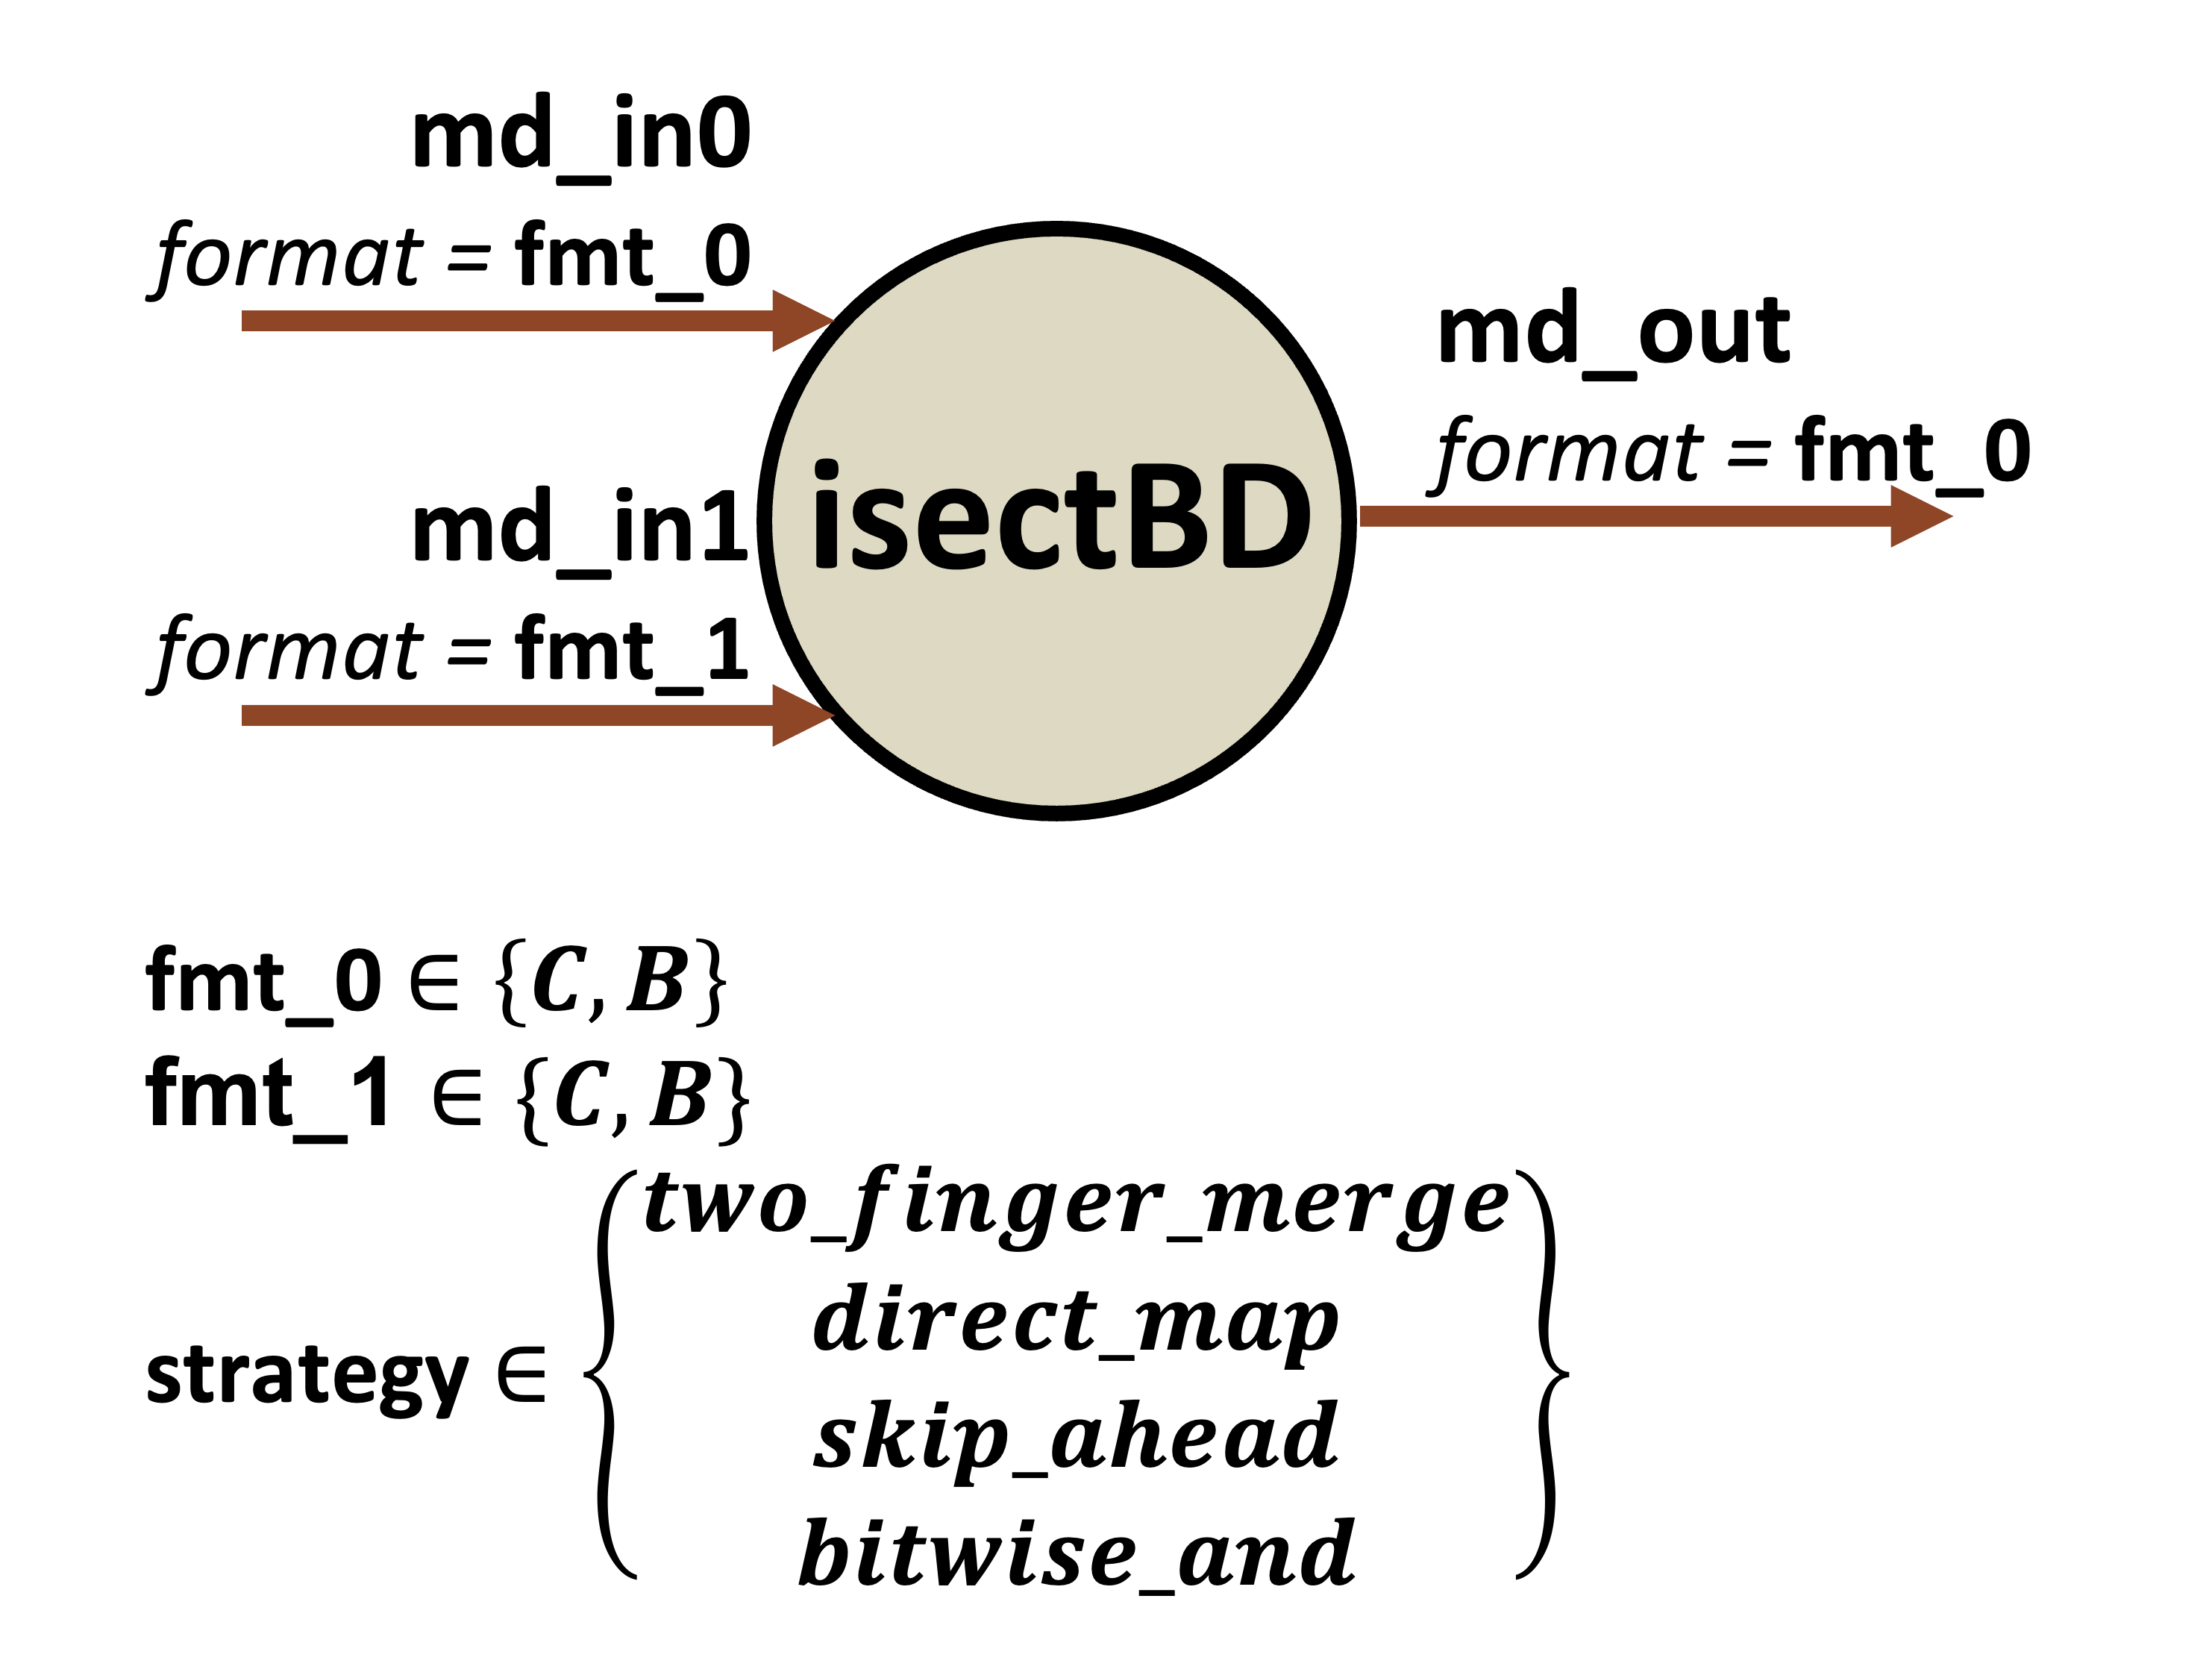
\includegraphics[width=0.95\textwidth]{figures/isectbd.png}
    \caption{Bidirectional intersection primitive component template.}
    \label{fig:isectbd}
\end{figure}

\begin{table}[H]
\centering
\begin{tabular}{lll}
\toprule
 format\_0   & format\_1   & strategy         \\
\midrule
 C          & C          & two\_finger\_merge \\
 C          & C          & skip\_ahead       \\
 C          & C          & direct\_map       \\
 B          & B          & bitwise\_and      \\
\bottomrule
\end{tabular}
\caption{Specializations of bidirectional intersection.}
\label{tab:IntersectionBidirectional_specializations}
\end{table}

\subsection{Fill optimizers}

\begin{figure}[H]
    \centering
    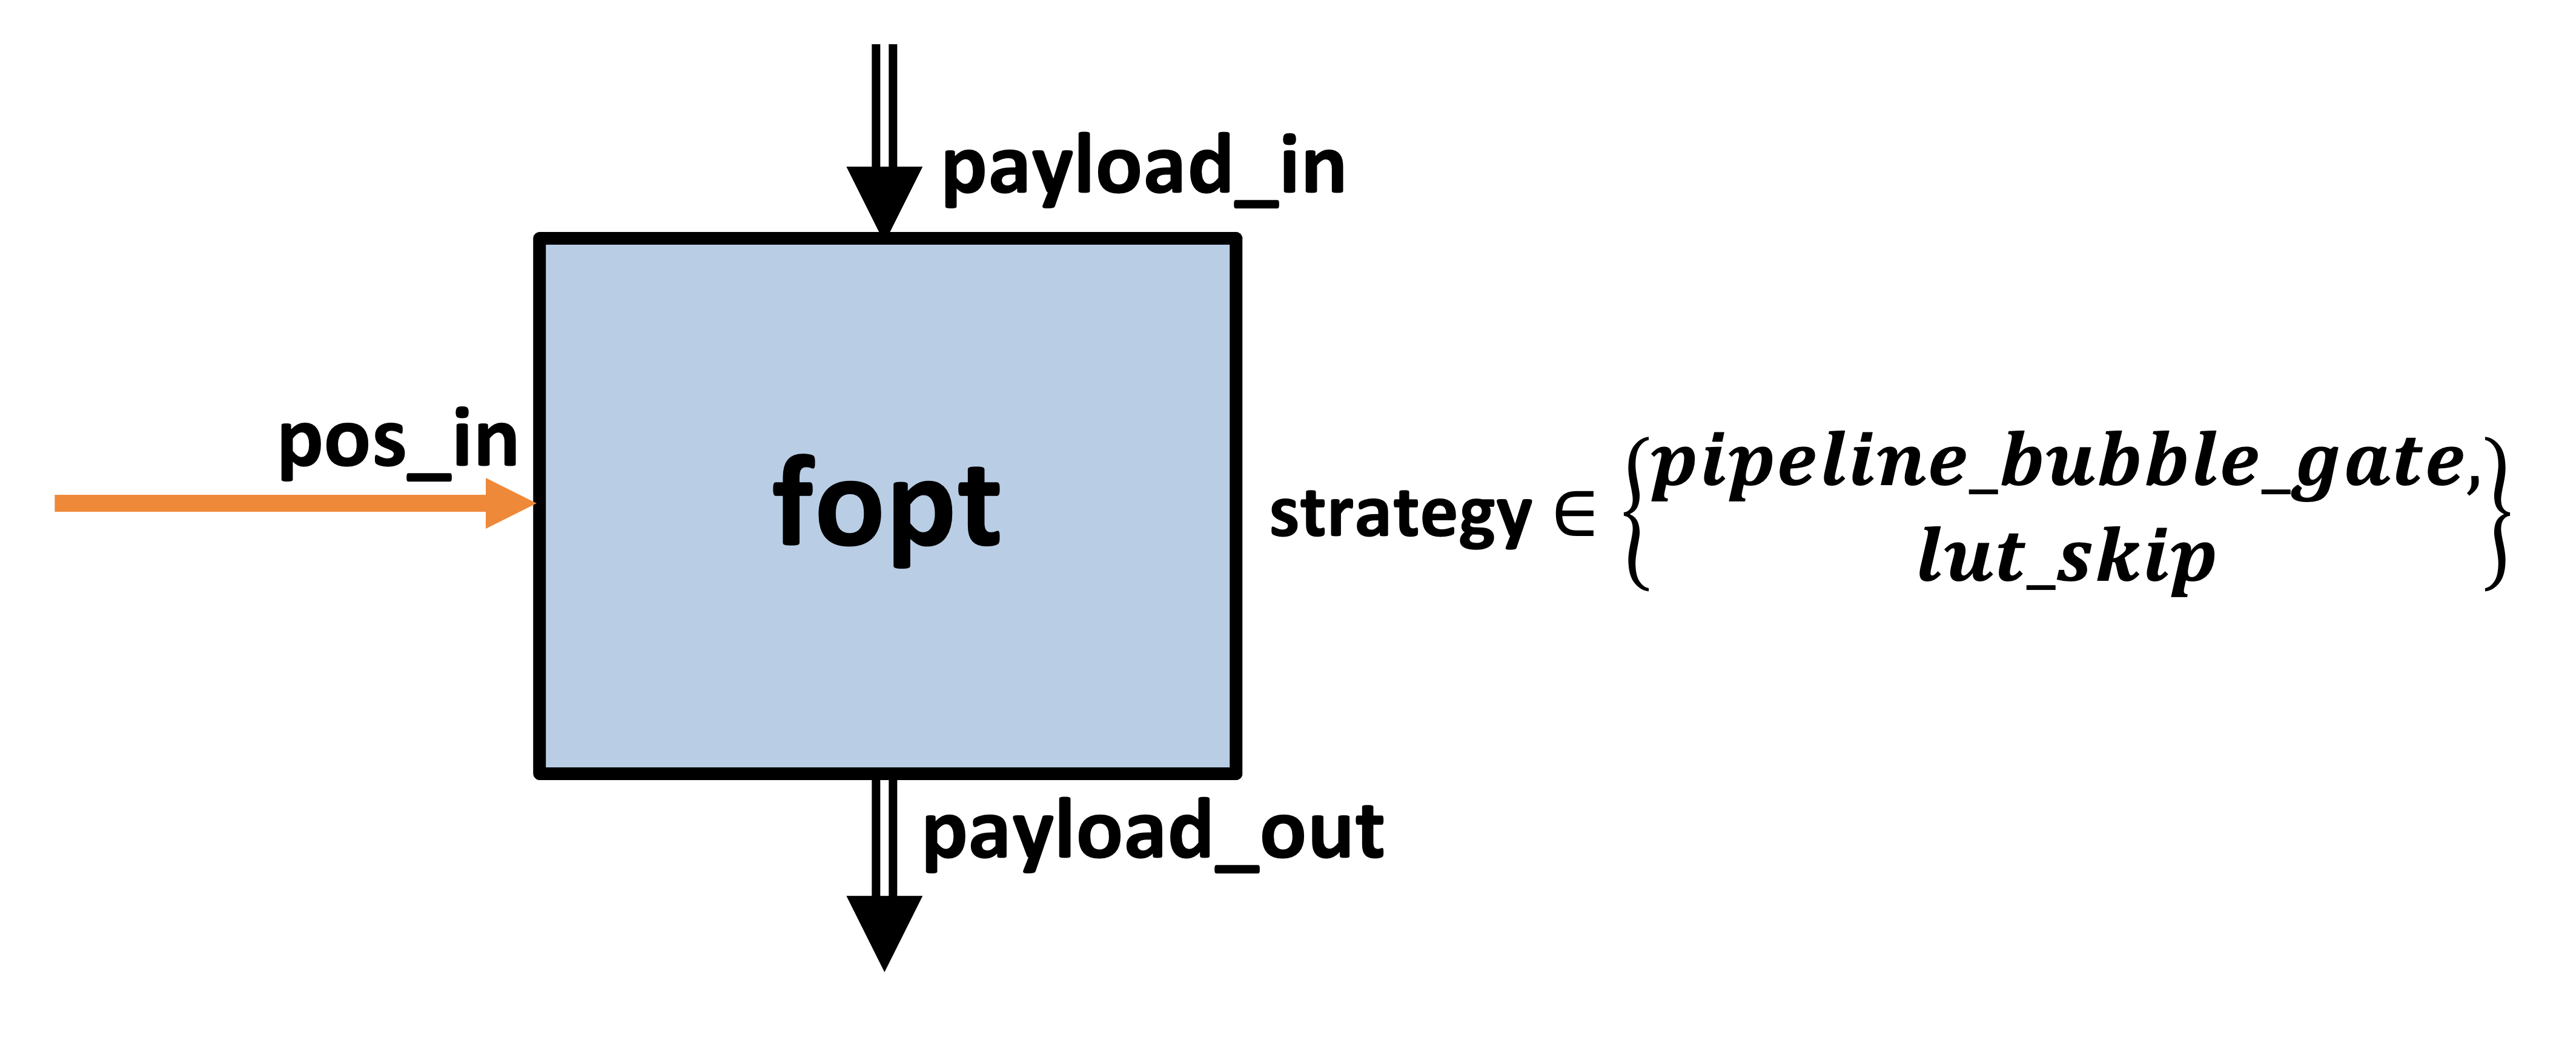
\includegraphics[width=0.95\textwidth]{figures/fopt.png}
    \caption{Fill optimizer primitive component template. The fill optimizer's (fopt's) method for discarding payload fills - as well as the interface between the fopt and the payload stream - is highly implementation-dependent, thus the fopt template does not have a ``payload'' interface. The red dotted line from fopt to payload stream is a visual cue for which payload stream is being optimized, but in actuality \textit{pos\_in} is the only interface port defined for this primitive component template.}
    \label{fig:fopt}
\end{figure}

\begin{table}[H]
\centering
\begin{tabular}{l}
\toprule
 strategy             \\
\midrule
 pipeline\_bubble\_gate \\
 lut\_skip             \\
\bottomrule
\end{tabular}
\caption{Specializations of fill optimizer}
\label{tab:FillOptimizer_specializations}
\end{table}

\section{SAF microarchitectures}

This section will overview the taxonomy of SAF microarchitectures considered in this work. SAF microarchitectures implement SAFs. Though not a requirement, in practice all SAF microarchitectures considered in this work were well-described as compound components, and conversely the only compound components modeled in this work happen to be SAF microarchitectures.

\subsection{Format microarchitectures}

\begin{figure}[H]
    \centering
    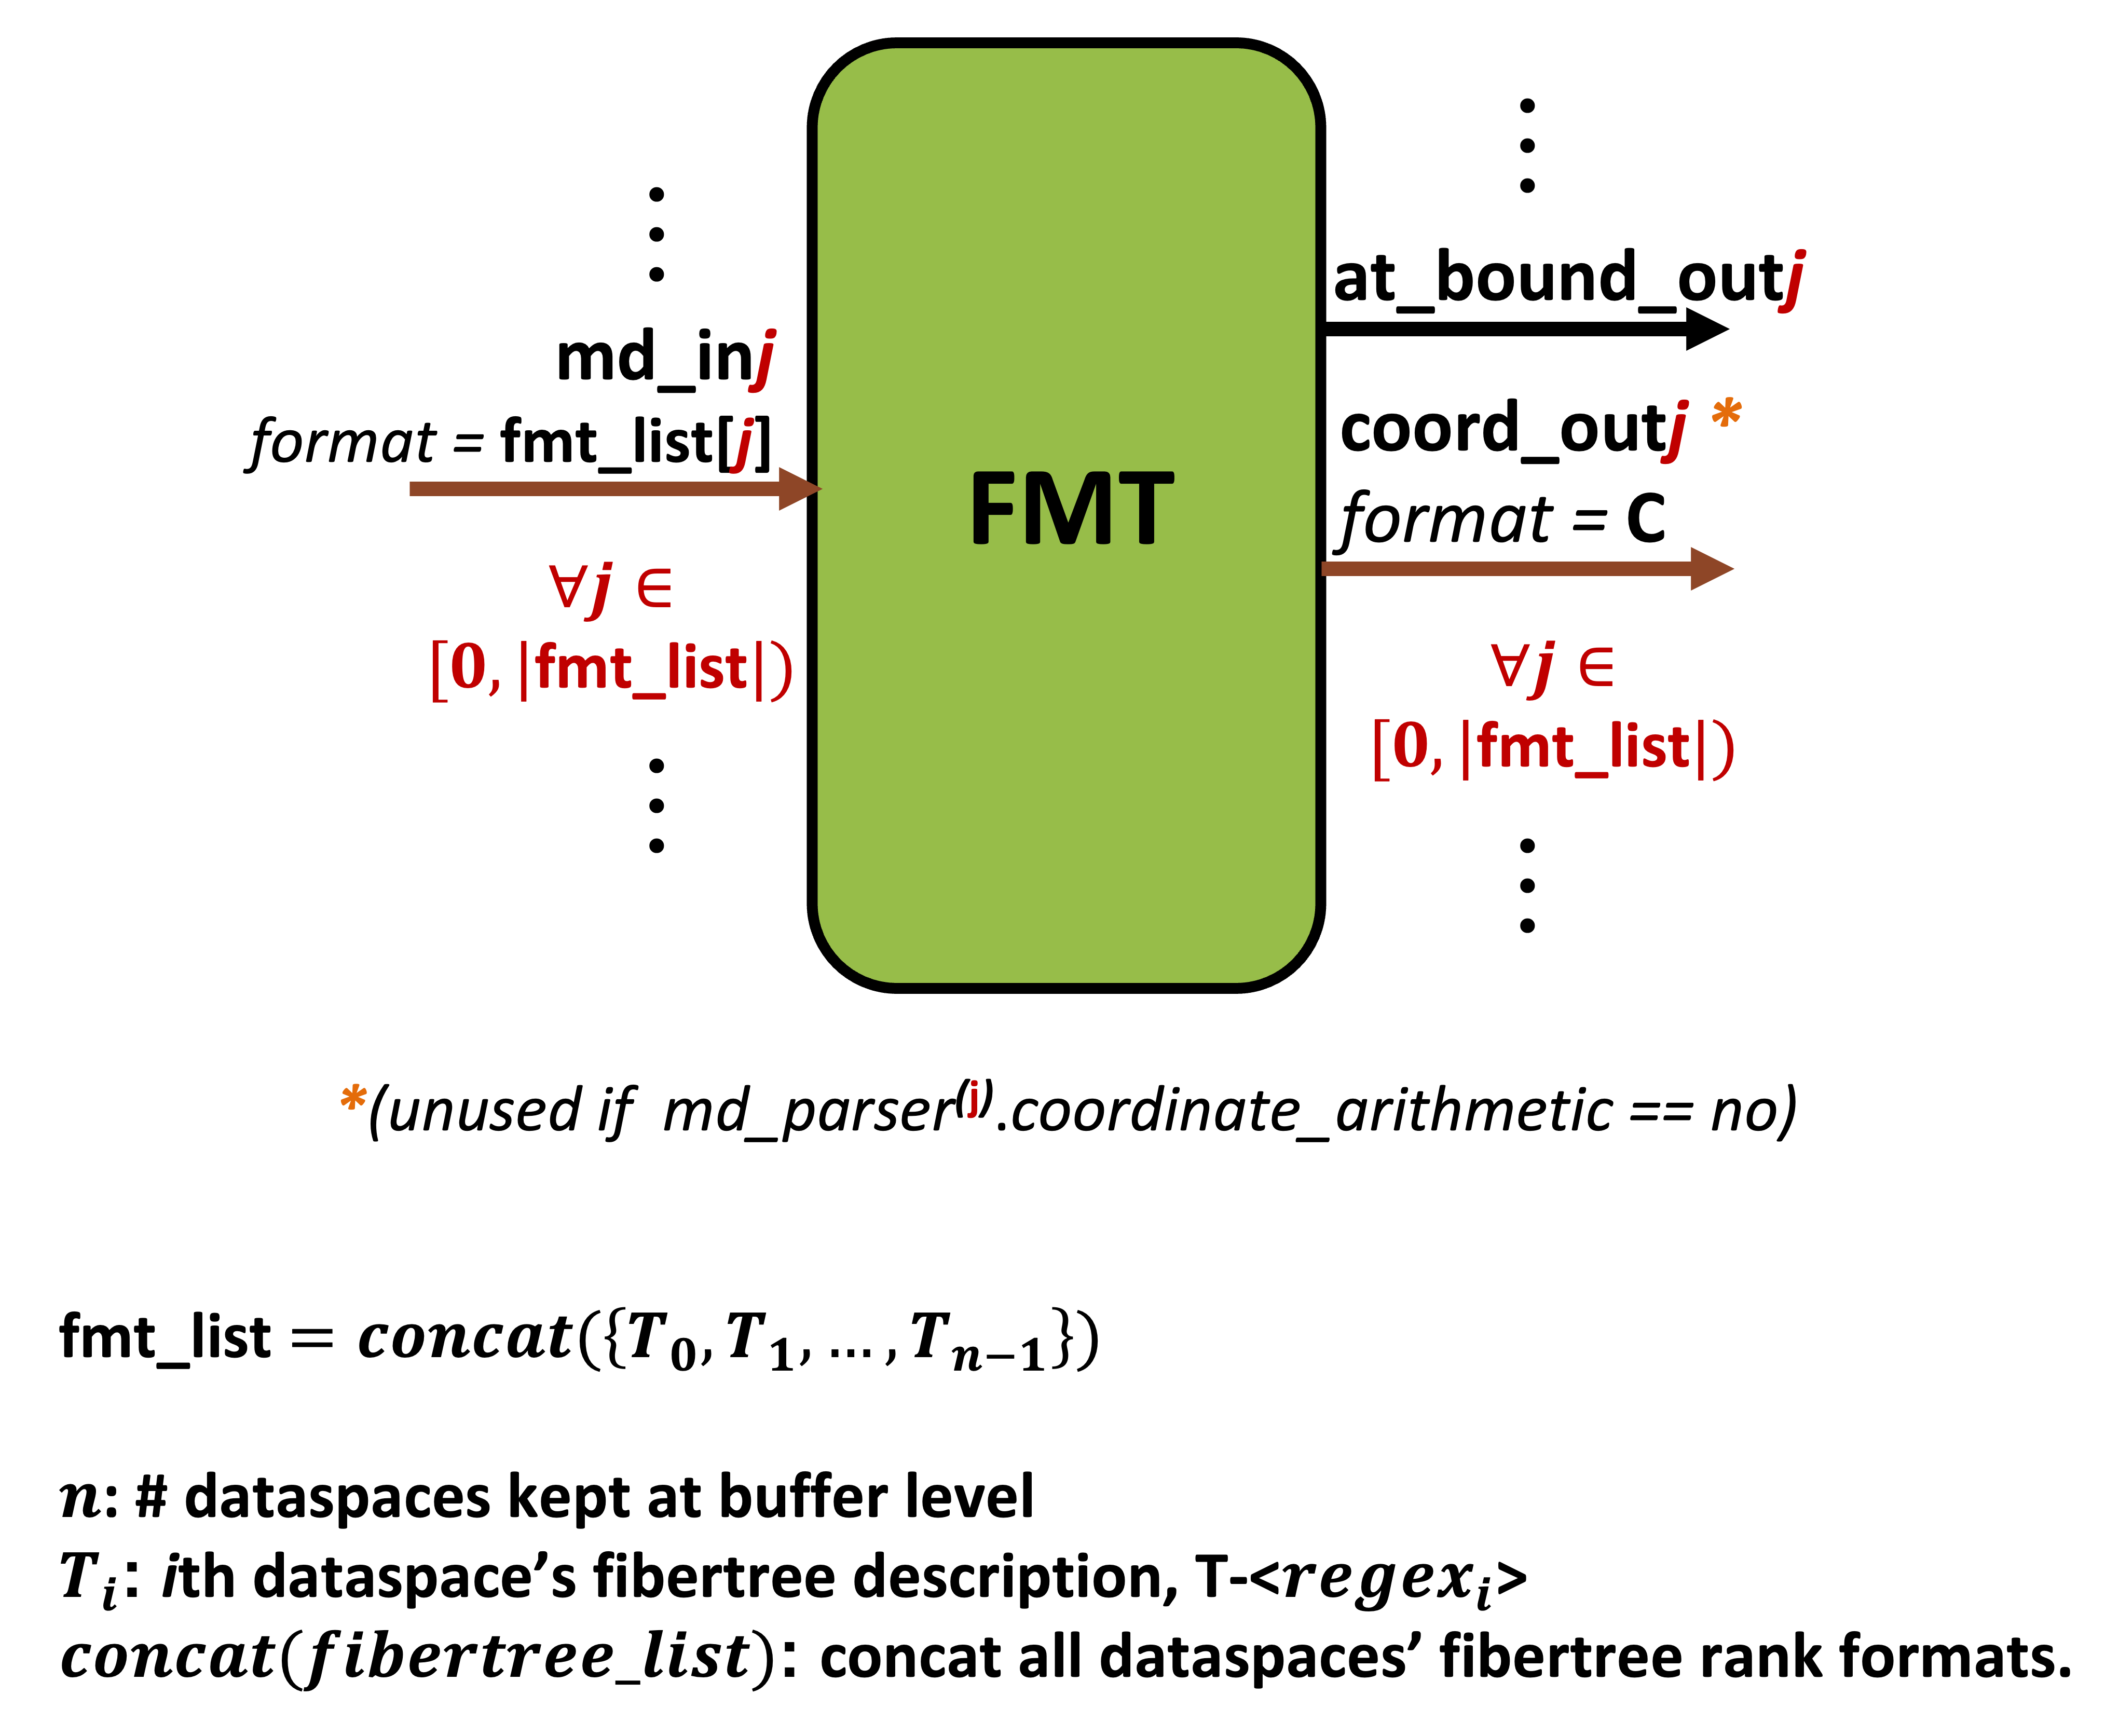
\includegraphics[width=0.95\textwidth]{figures/FMT.png}
    \caption{Format microarchitecture compound component template. If an architectural buffer has a format SAF, a format microarchitecture must be bound to it. The fmt\_list parameter expects a list of rank formats. The architectural buffer keeps\cite{timeloop} one or more dataspaces\cite{timeloop}, at least one of which exploits a format SAF. fmt\_list is assumed to have been derived from concatenating the fiber representation regexes\cite{szebook} for all kept dataspaces' fibertrees, excluding dataspaces which do not exploit a format SAF.}
    \label{fig:FMT}
\end{figure}

%\begin{table}[H]
%\centering
%\begin{tabular}{l}
%\toprule
% fibertree   \\
%\midrule
% *           \\
%\bottomrule
%\end{tabular}
%\caption{Specializations of format microarchitecture}
%\label{tab:format_microarchitecture_specializations}
%\end{table}

\begin{figure}[H]
    \centering
    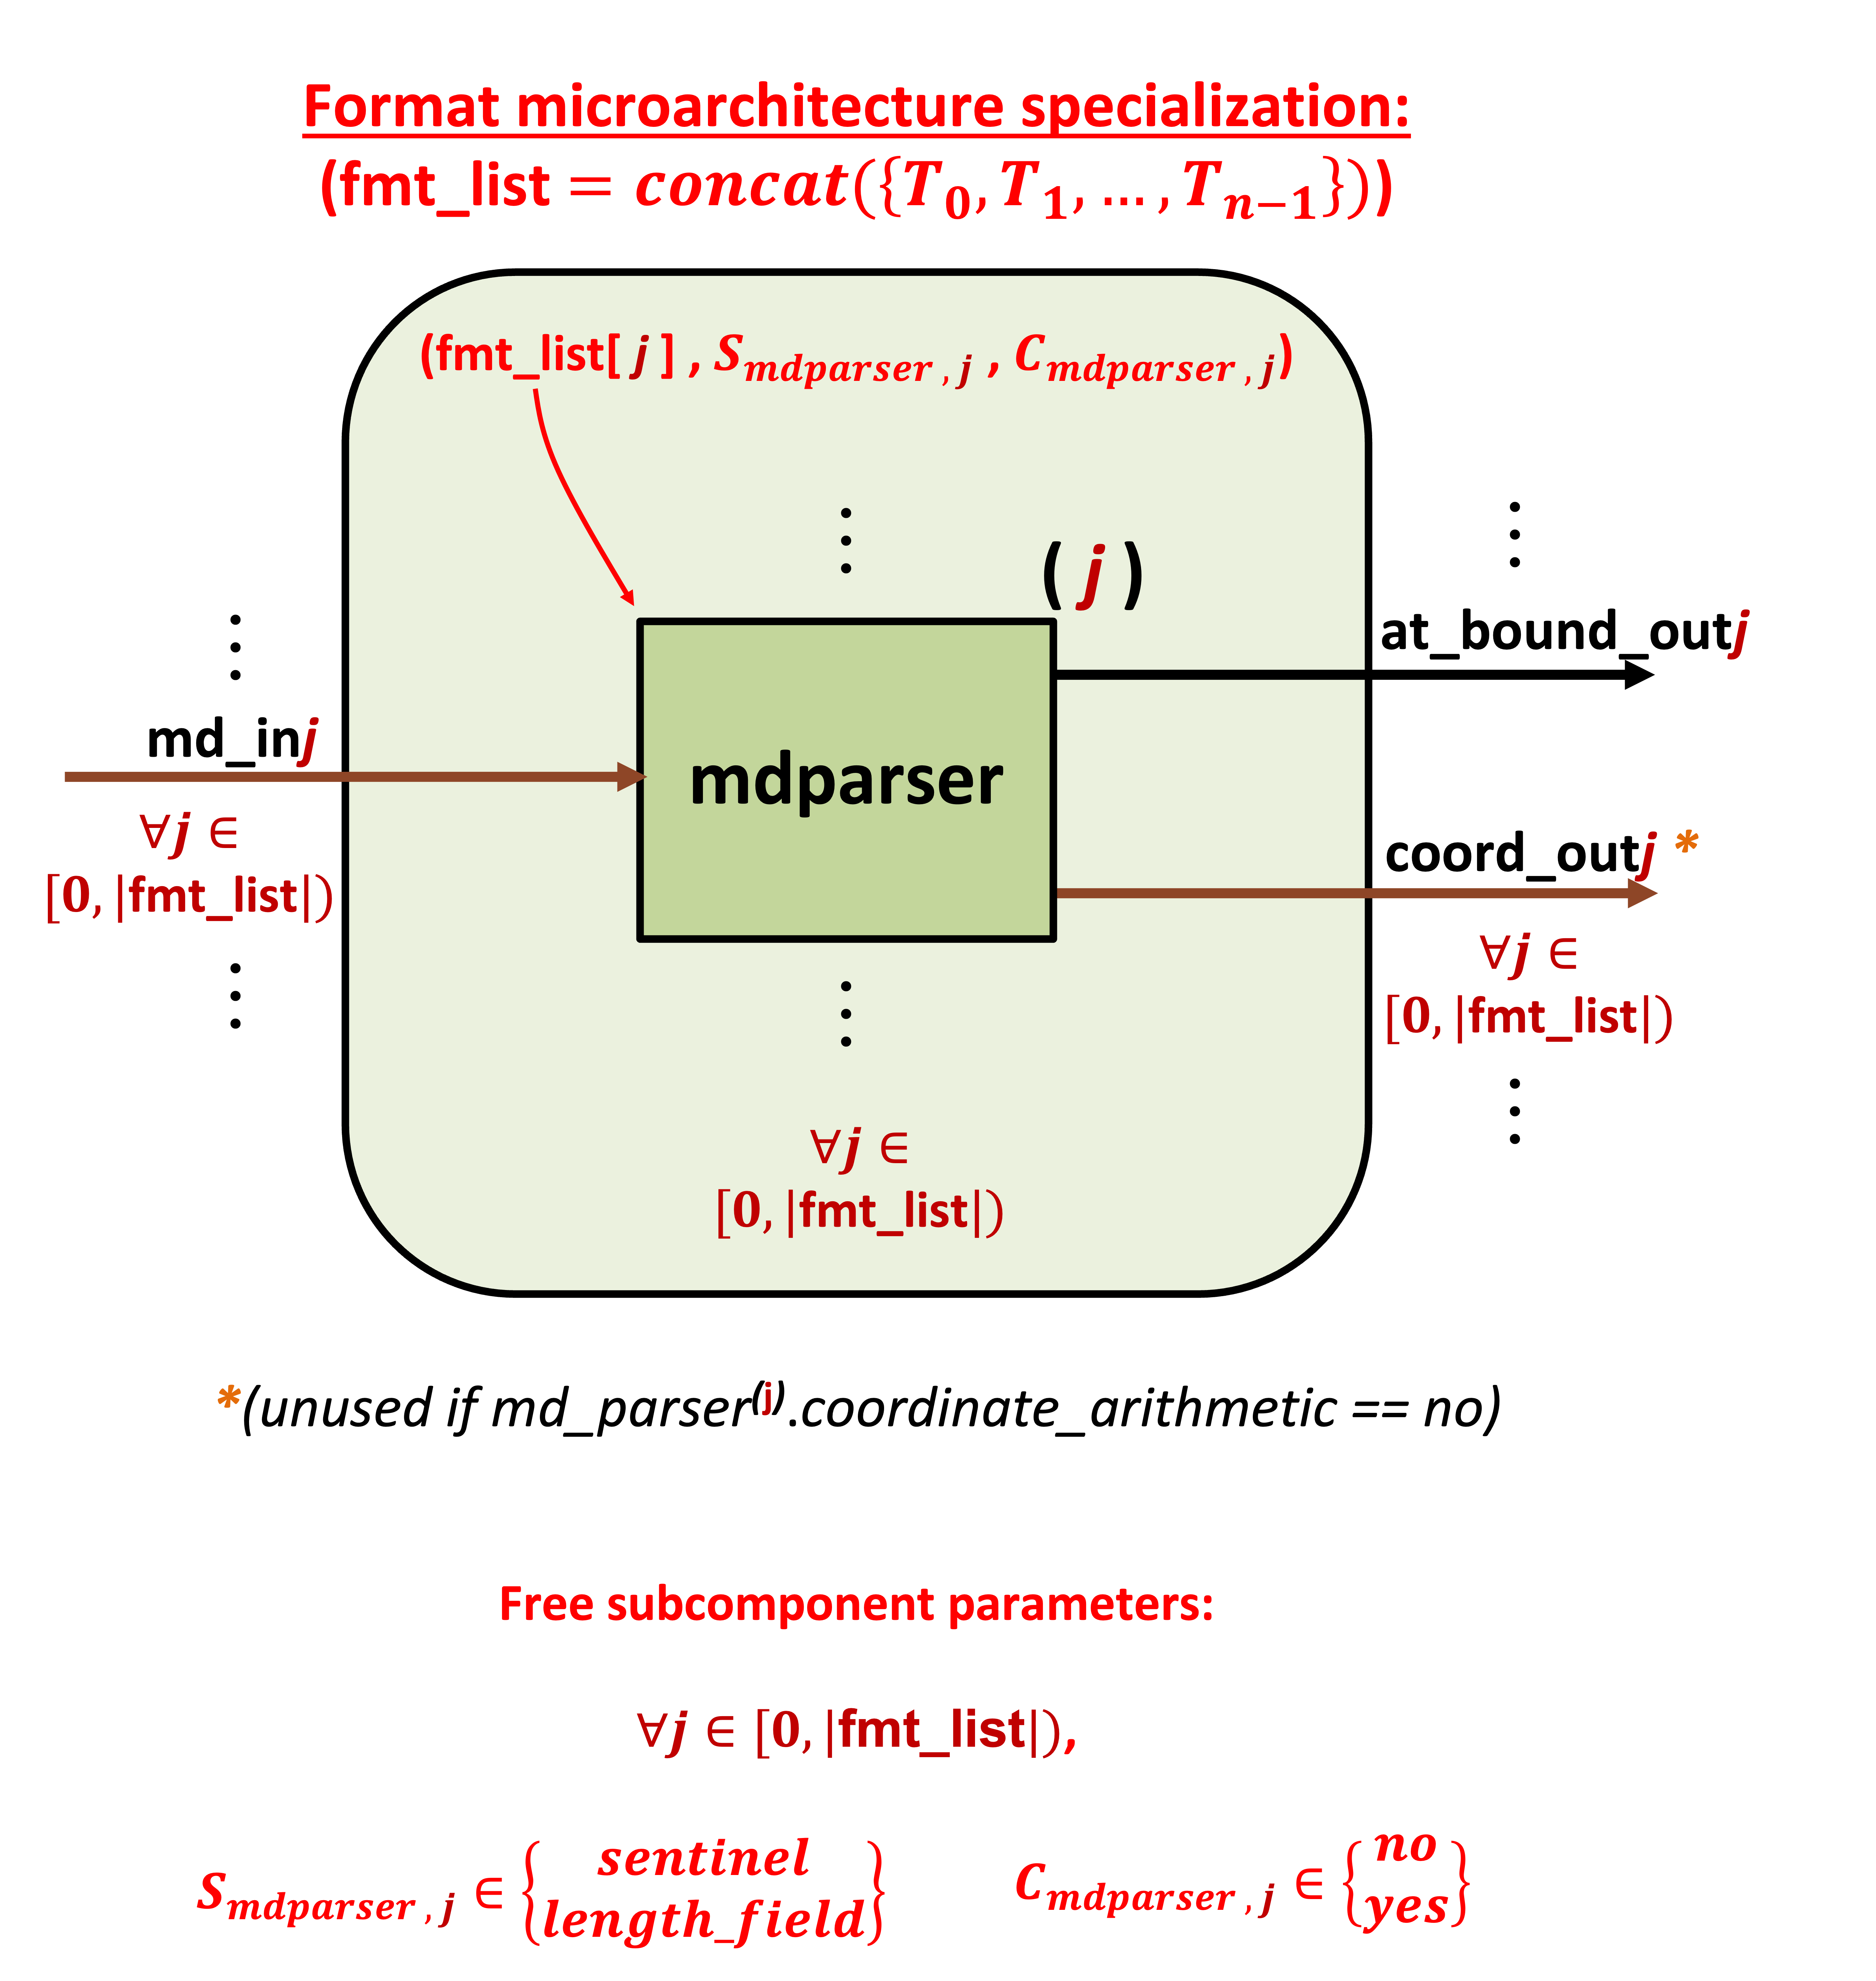
\includegraphics[width=0.95\textwidth]{figures/FMT_all.png}
    \caption{Format microarchitecture implementation topology. Every rank, in every fibertree, in every kept dataspace which is subject to a format SAF for a given buffer, has a corresponding metadata parser in the format microarchitecture topology. This implementation topology is universal for format microarchitectures regardless of the specific \textit{fmt\_list} parameter value. Each metadata parser subcomponent, however, has two free parameters. Setting \textit{coordinate\_arithmetic = no} for the $j$th metadata parser, means that that format microarchitecture will not support coordinate arithmetic for the corresponding fibertree rank. This can conserve resources i.e. if the rank is being contracted anyway.}
    \label{fig:FMT_all}
\end{figure}

\subsection{Skipping microarchitectures}

\begin{figure}[H]
    \centering
    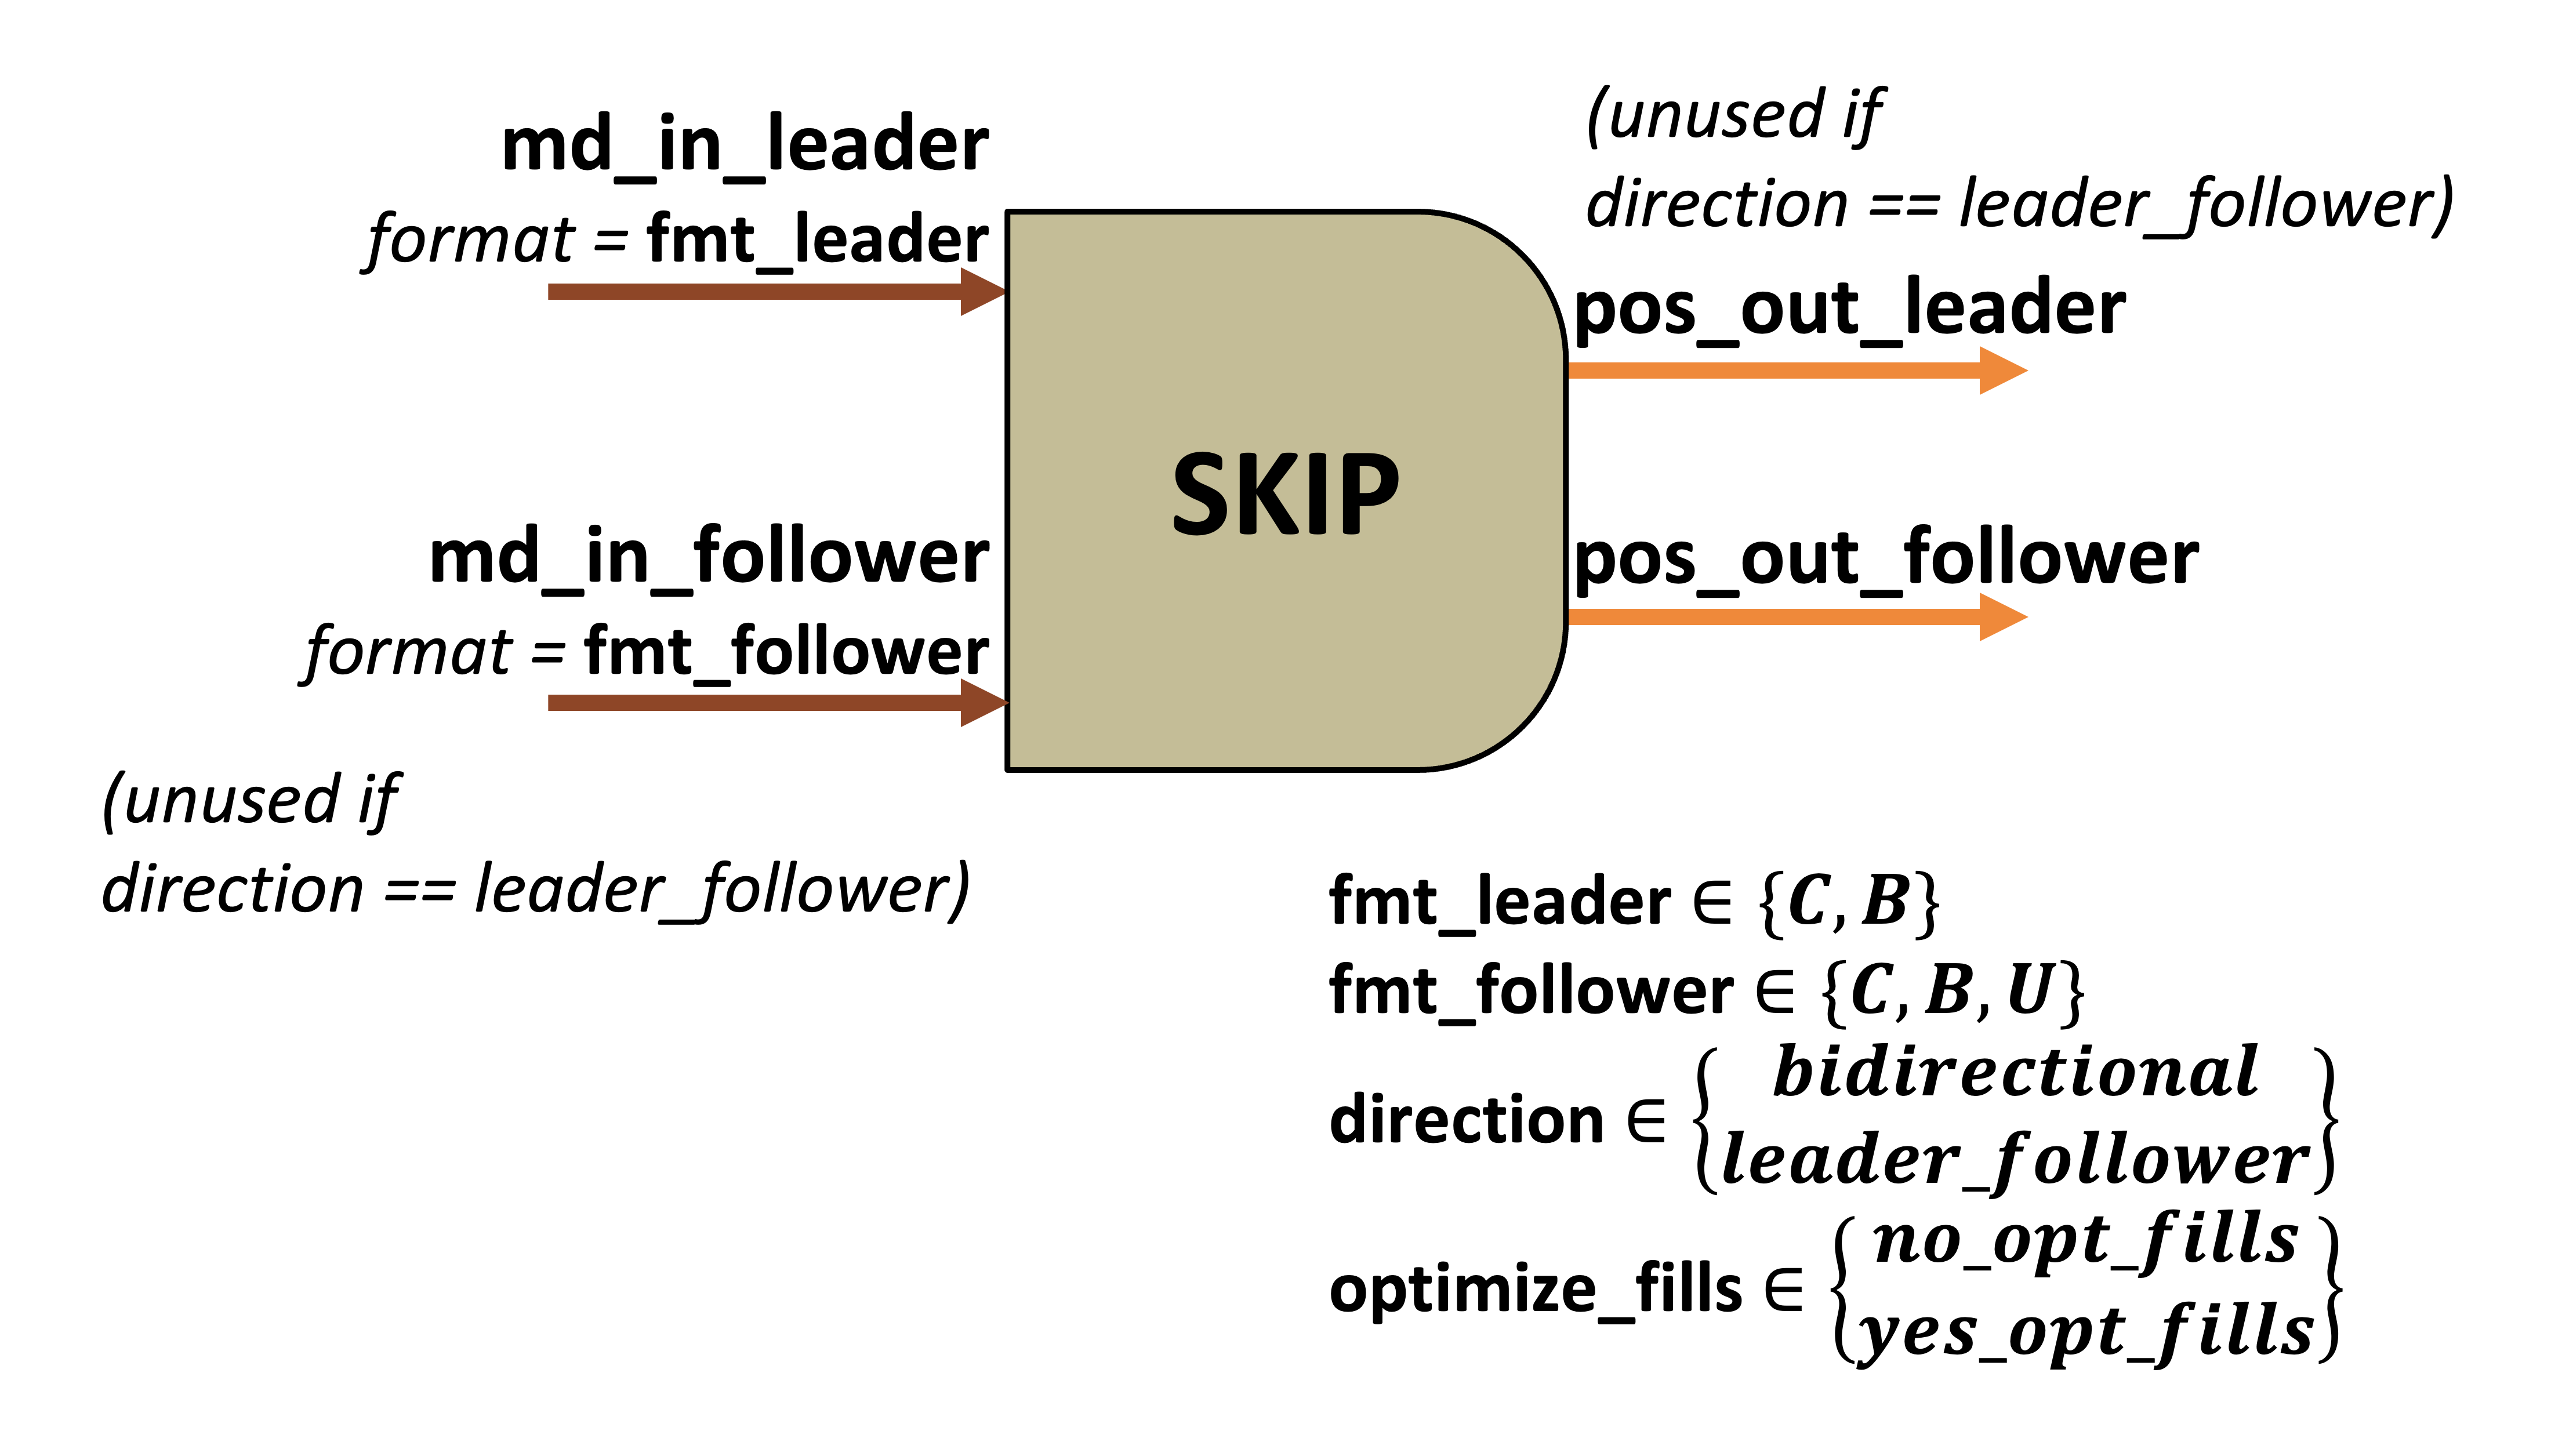
\includegraphics[width=0.95\textwidth]{figures/SKIP.png}
    \caption{Skipping microarchitecture compound component template.}
    \label{fig:SKIP}
\end{figure}

\subsubsection{Skipping microarchitecture specializations}

\begin{table}[ht]
\centering
\begin{tabular}{llll}
\toprule
 format\_leader   & format\_follower   & direction       & optimize\_fills   \\
\midrule
 C               & C                 & bidirectional   & no\_opt\_fills     \\
 B               & B                 & bidirectional   & no\_opt\_fills     \\
 C               & U                 & leader\_follower & no\_opt\_fills     \\
 C               & U                 & leader\_follower & yes\_opt\_fills    \\
\bottomrule
\end{tabular}
\caption{Specializations of skipping microarchitecture}
\label{tab:Skipping microarchitecture_specializations}
\end{table}

\begin{figure}[H]
    \centering
    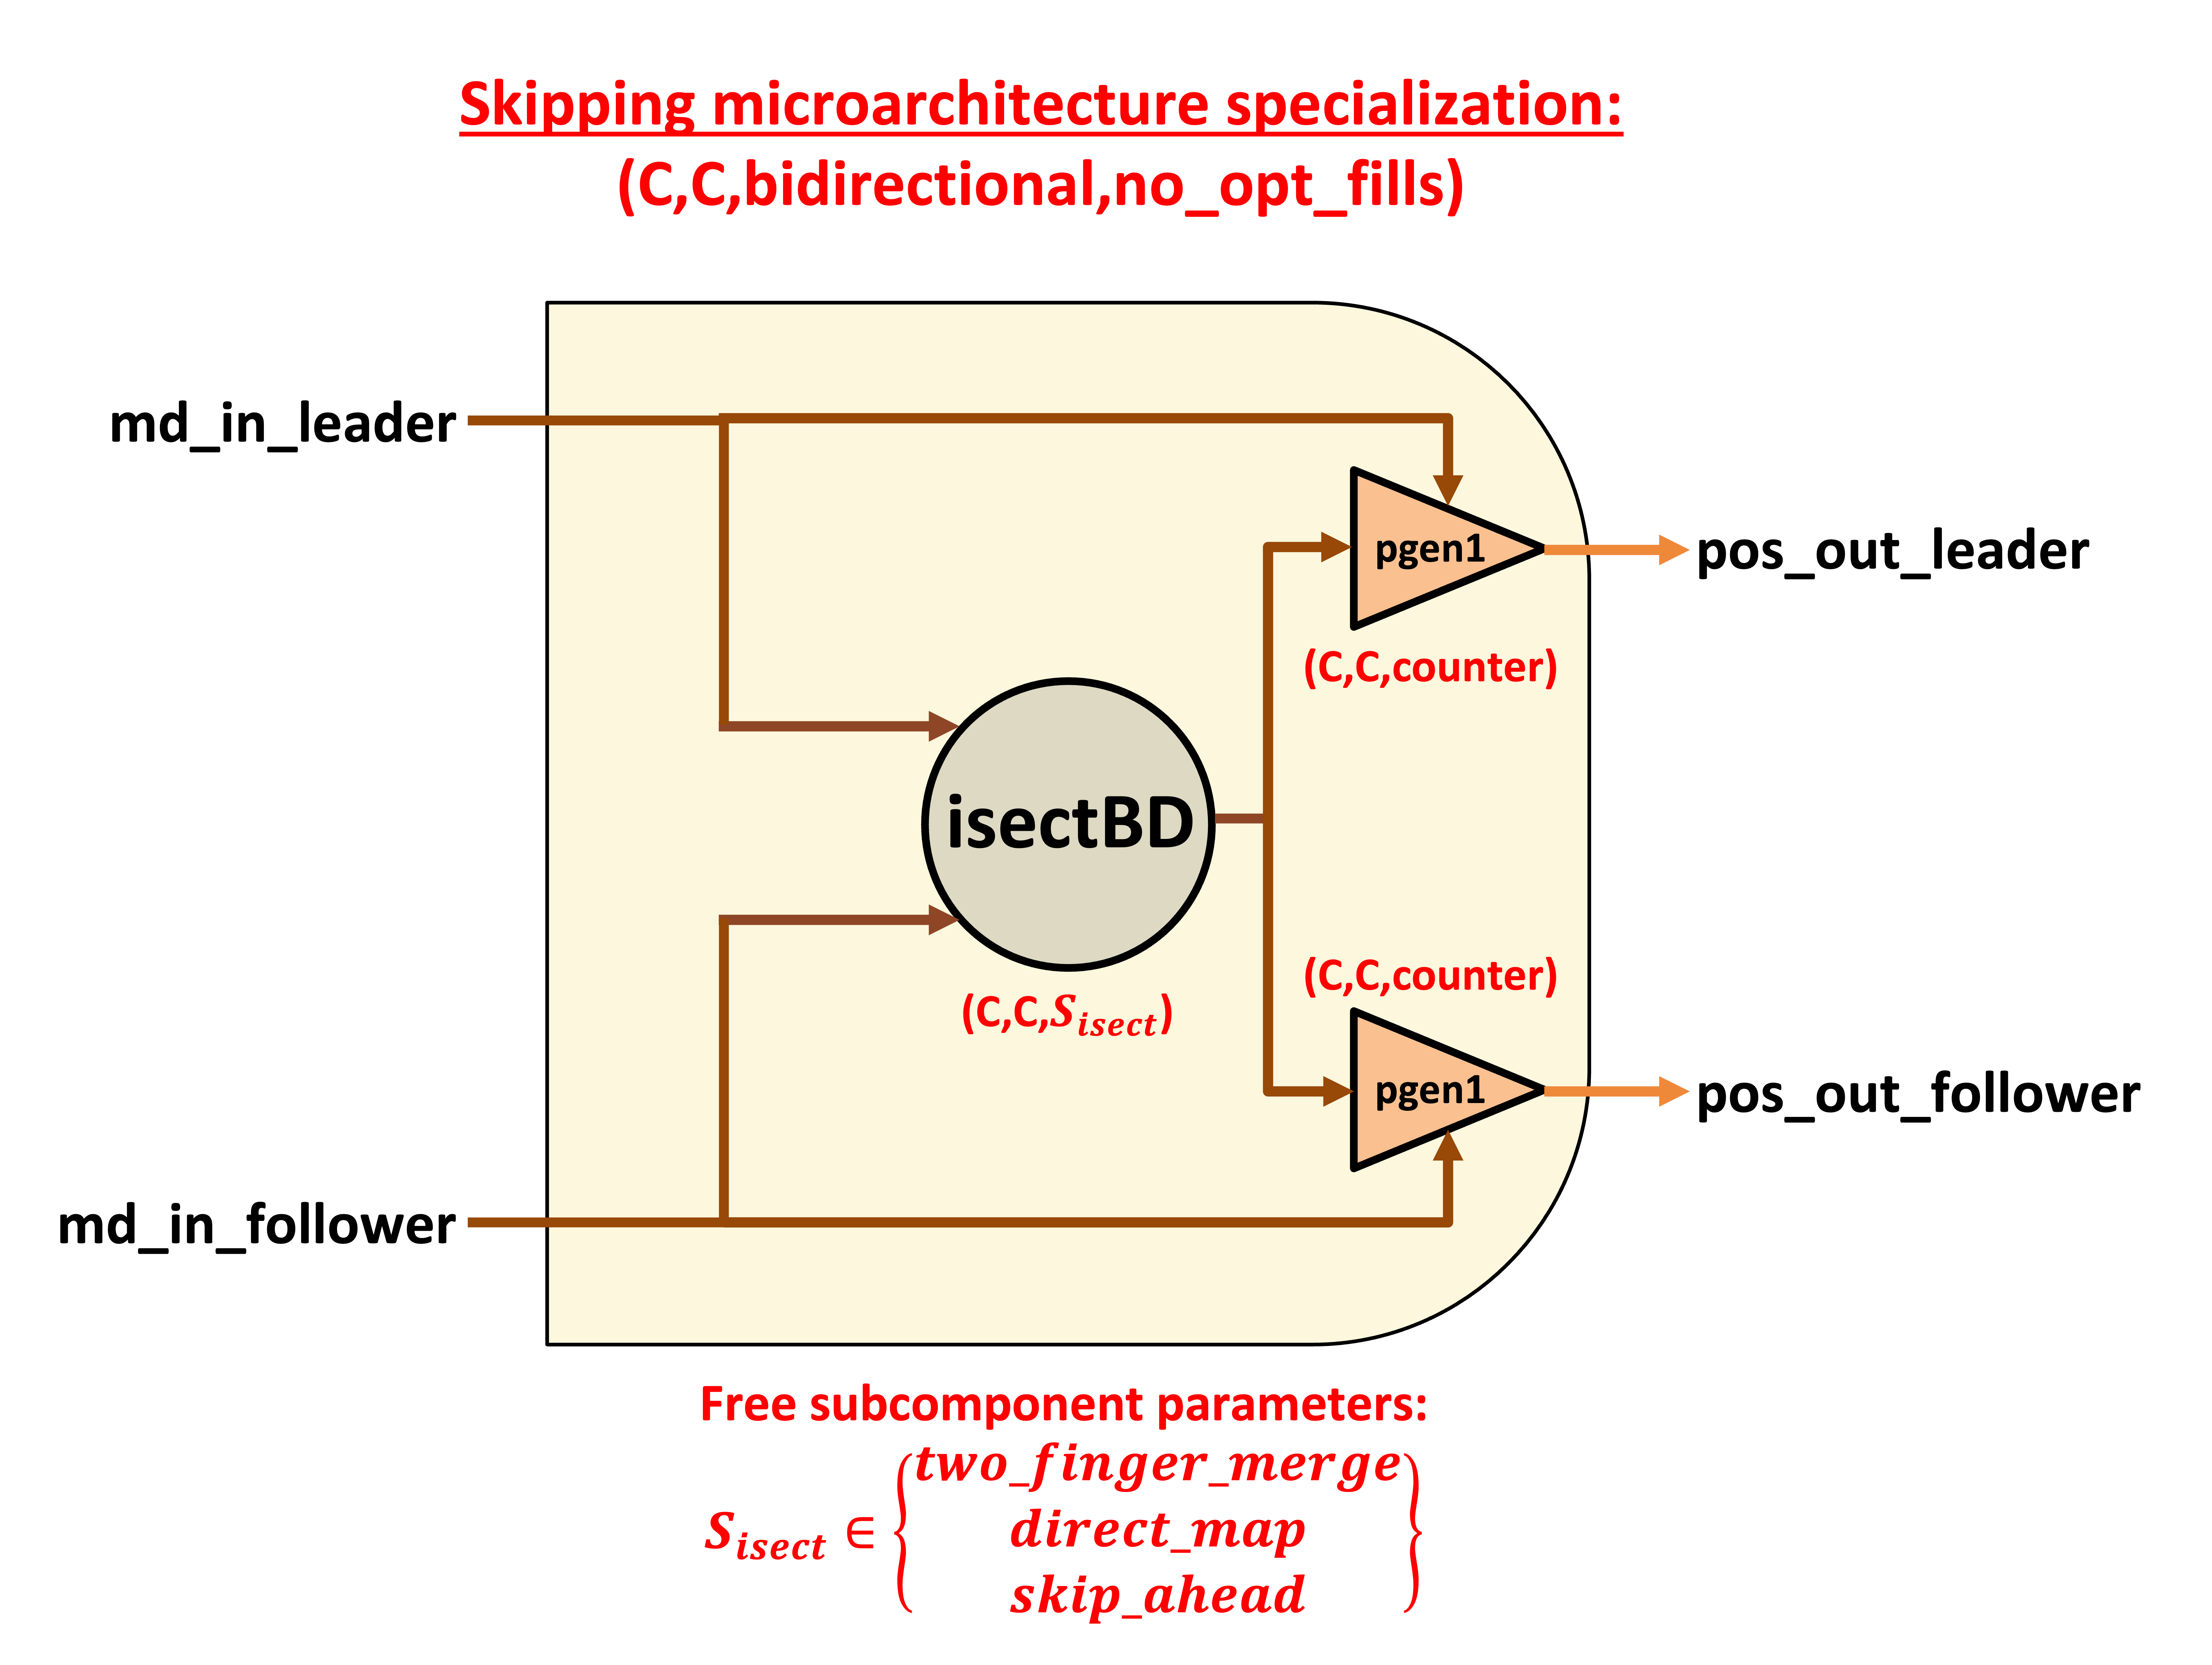
\includegraphics[width=0.95\textwidth]{figures/SKIP_C_C_bidirectional_no_opt_fills.png}
    \caption{Bidirectional coordinate-payload (C) skipping microarchitecture implementation topology (``ExTensor-like''\cite{extensor}.)}
    \label{fig:SKIP_C_C_bidirectional_no_opt_fills}
\end{figure}

\begin{figure}[H]
    \centering
    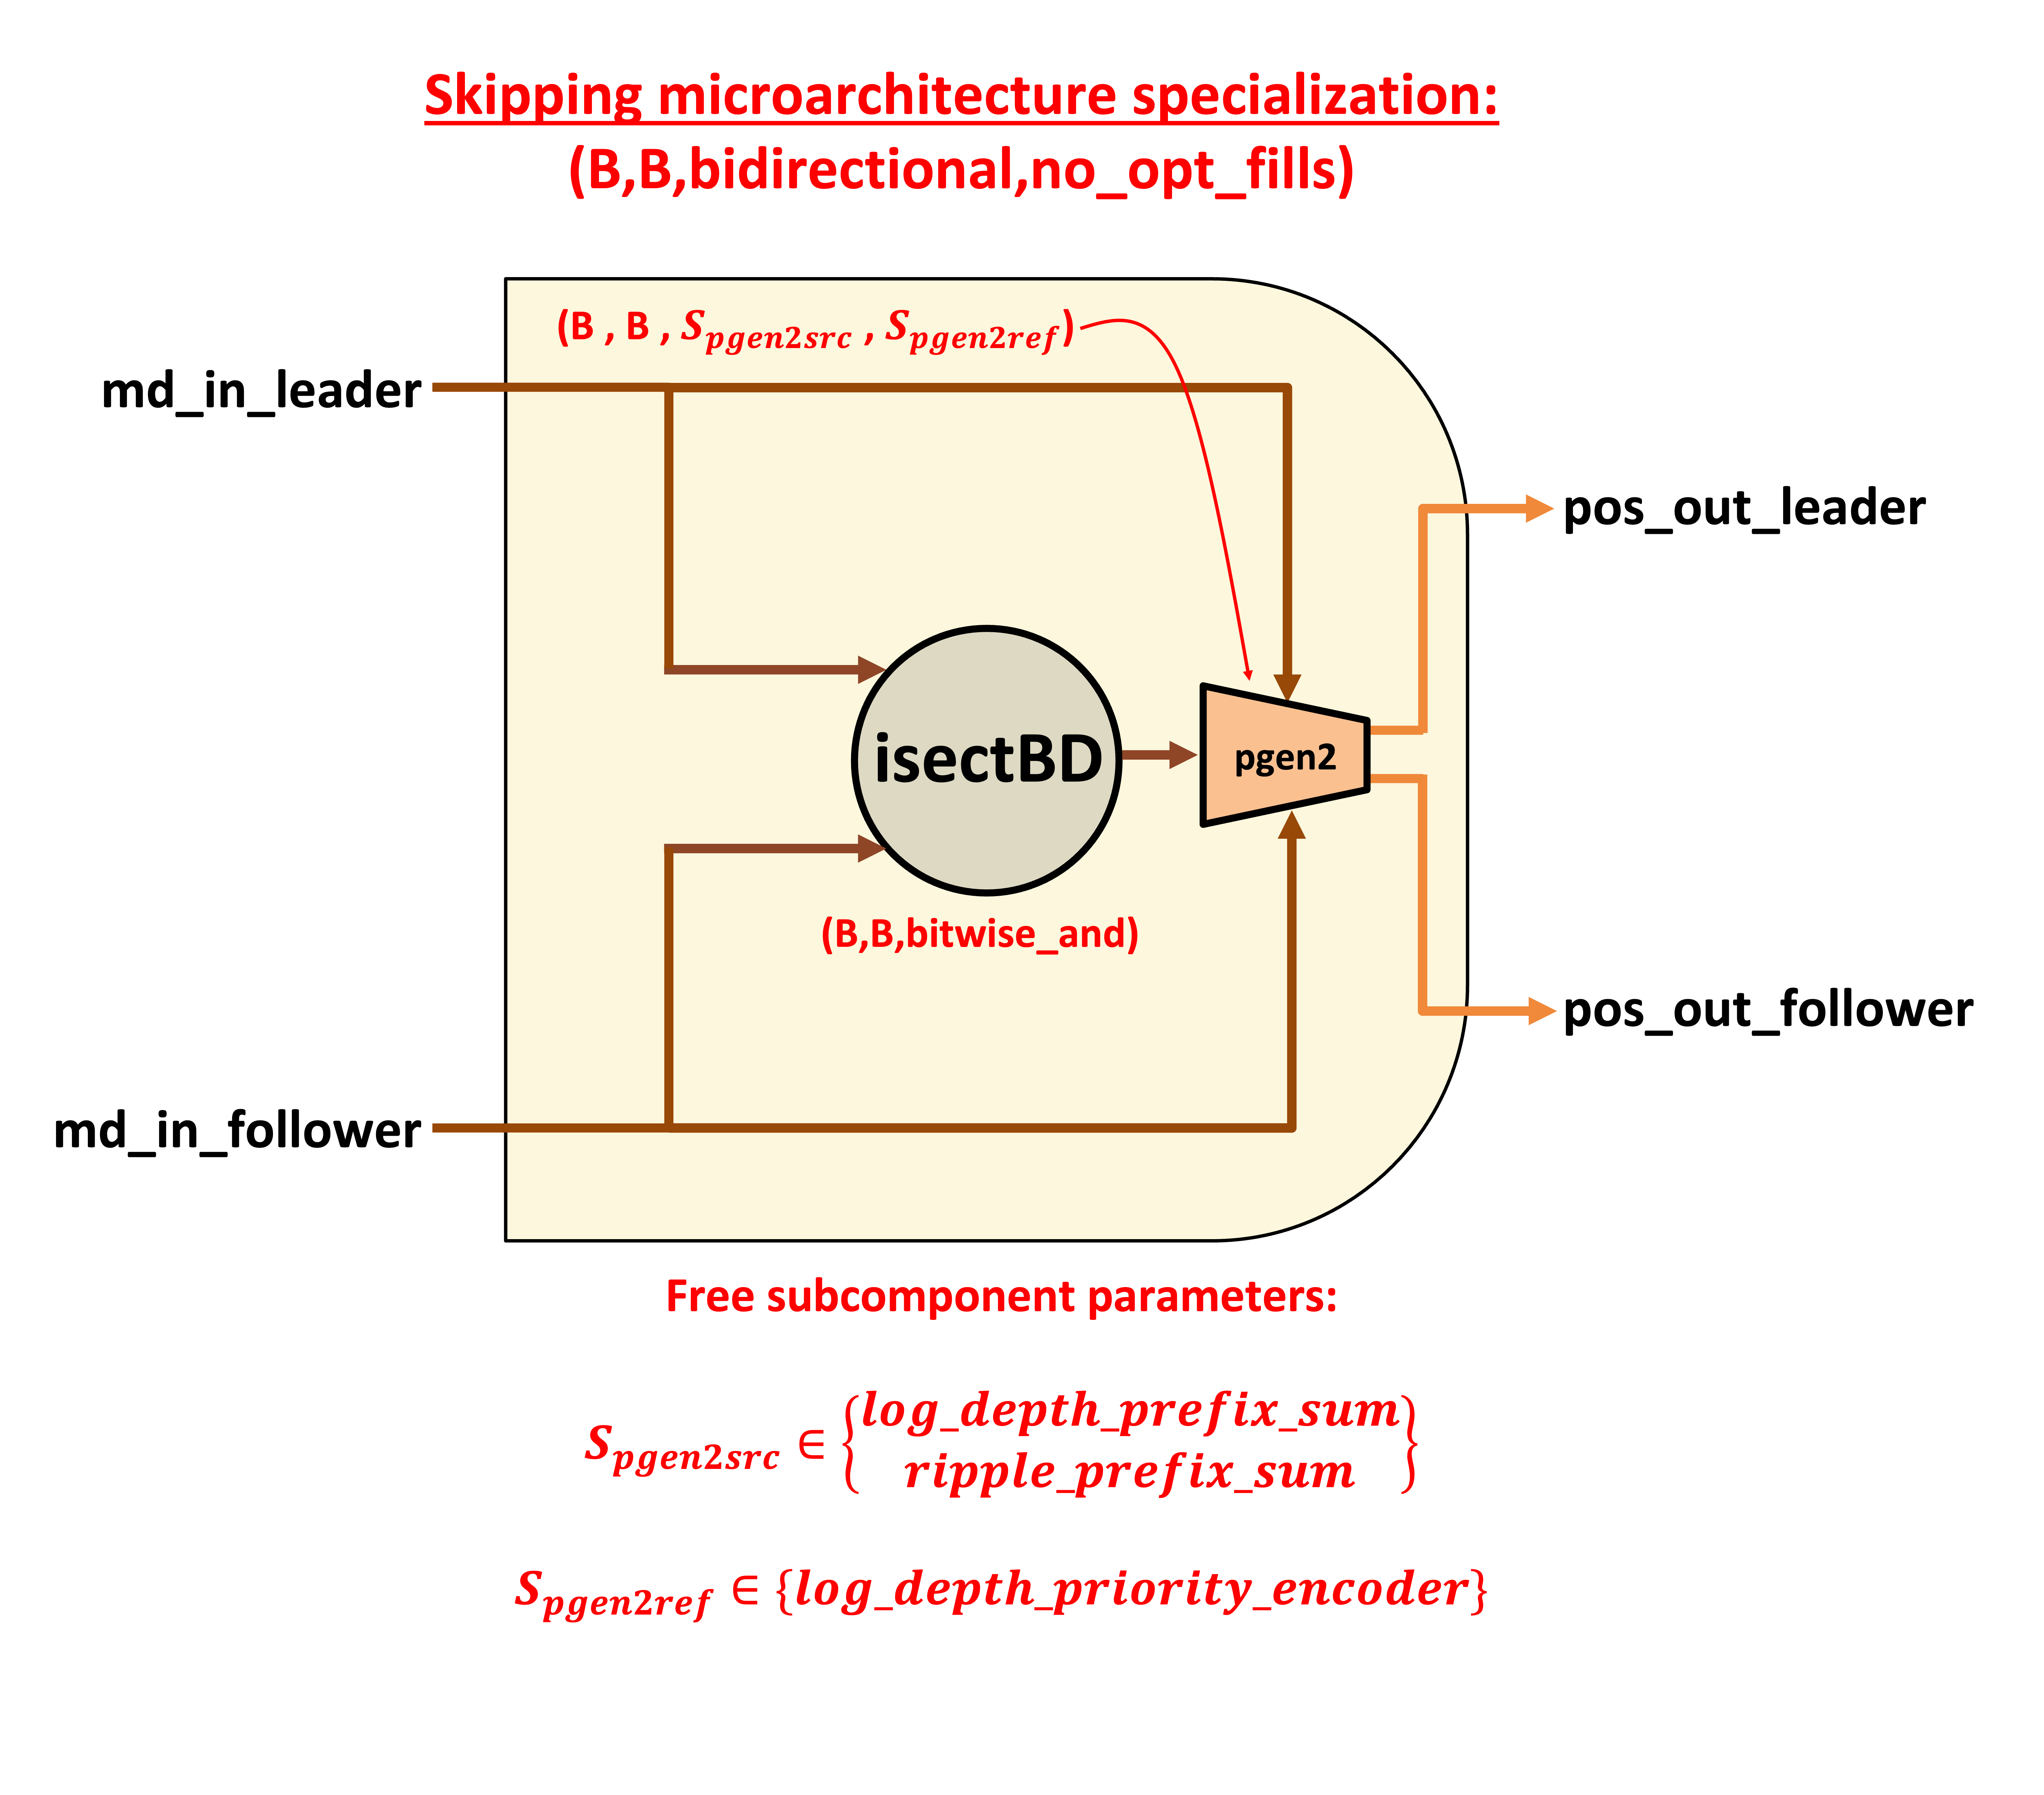
\includegraphics[width=0.95\textwidth]{figures/SKIP_B_B_bidirectional_no_opt_fills.png}
    \caption{Bidirectional bitmask (B) skipping microarchitecture implementation topology (``SparTen-like''\cite{sparten}.)}
    \label{fig:SKIP_B_B_bidirectional_no_opt_fills}
\end{figure}

\begin{figure}[H]
    \centering
    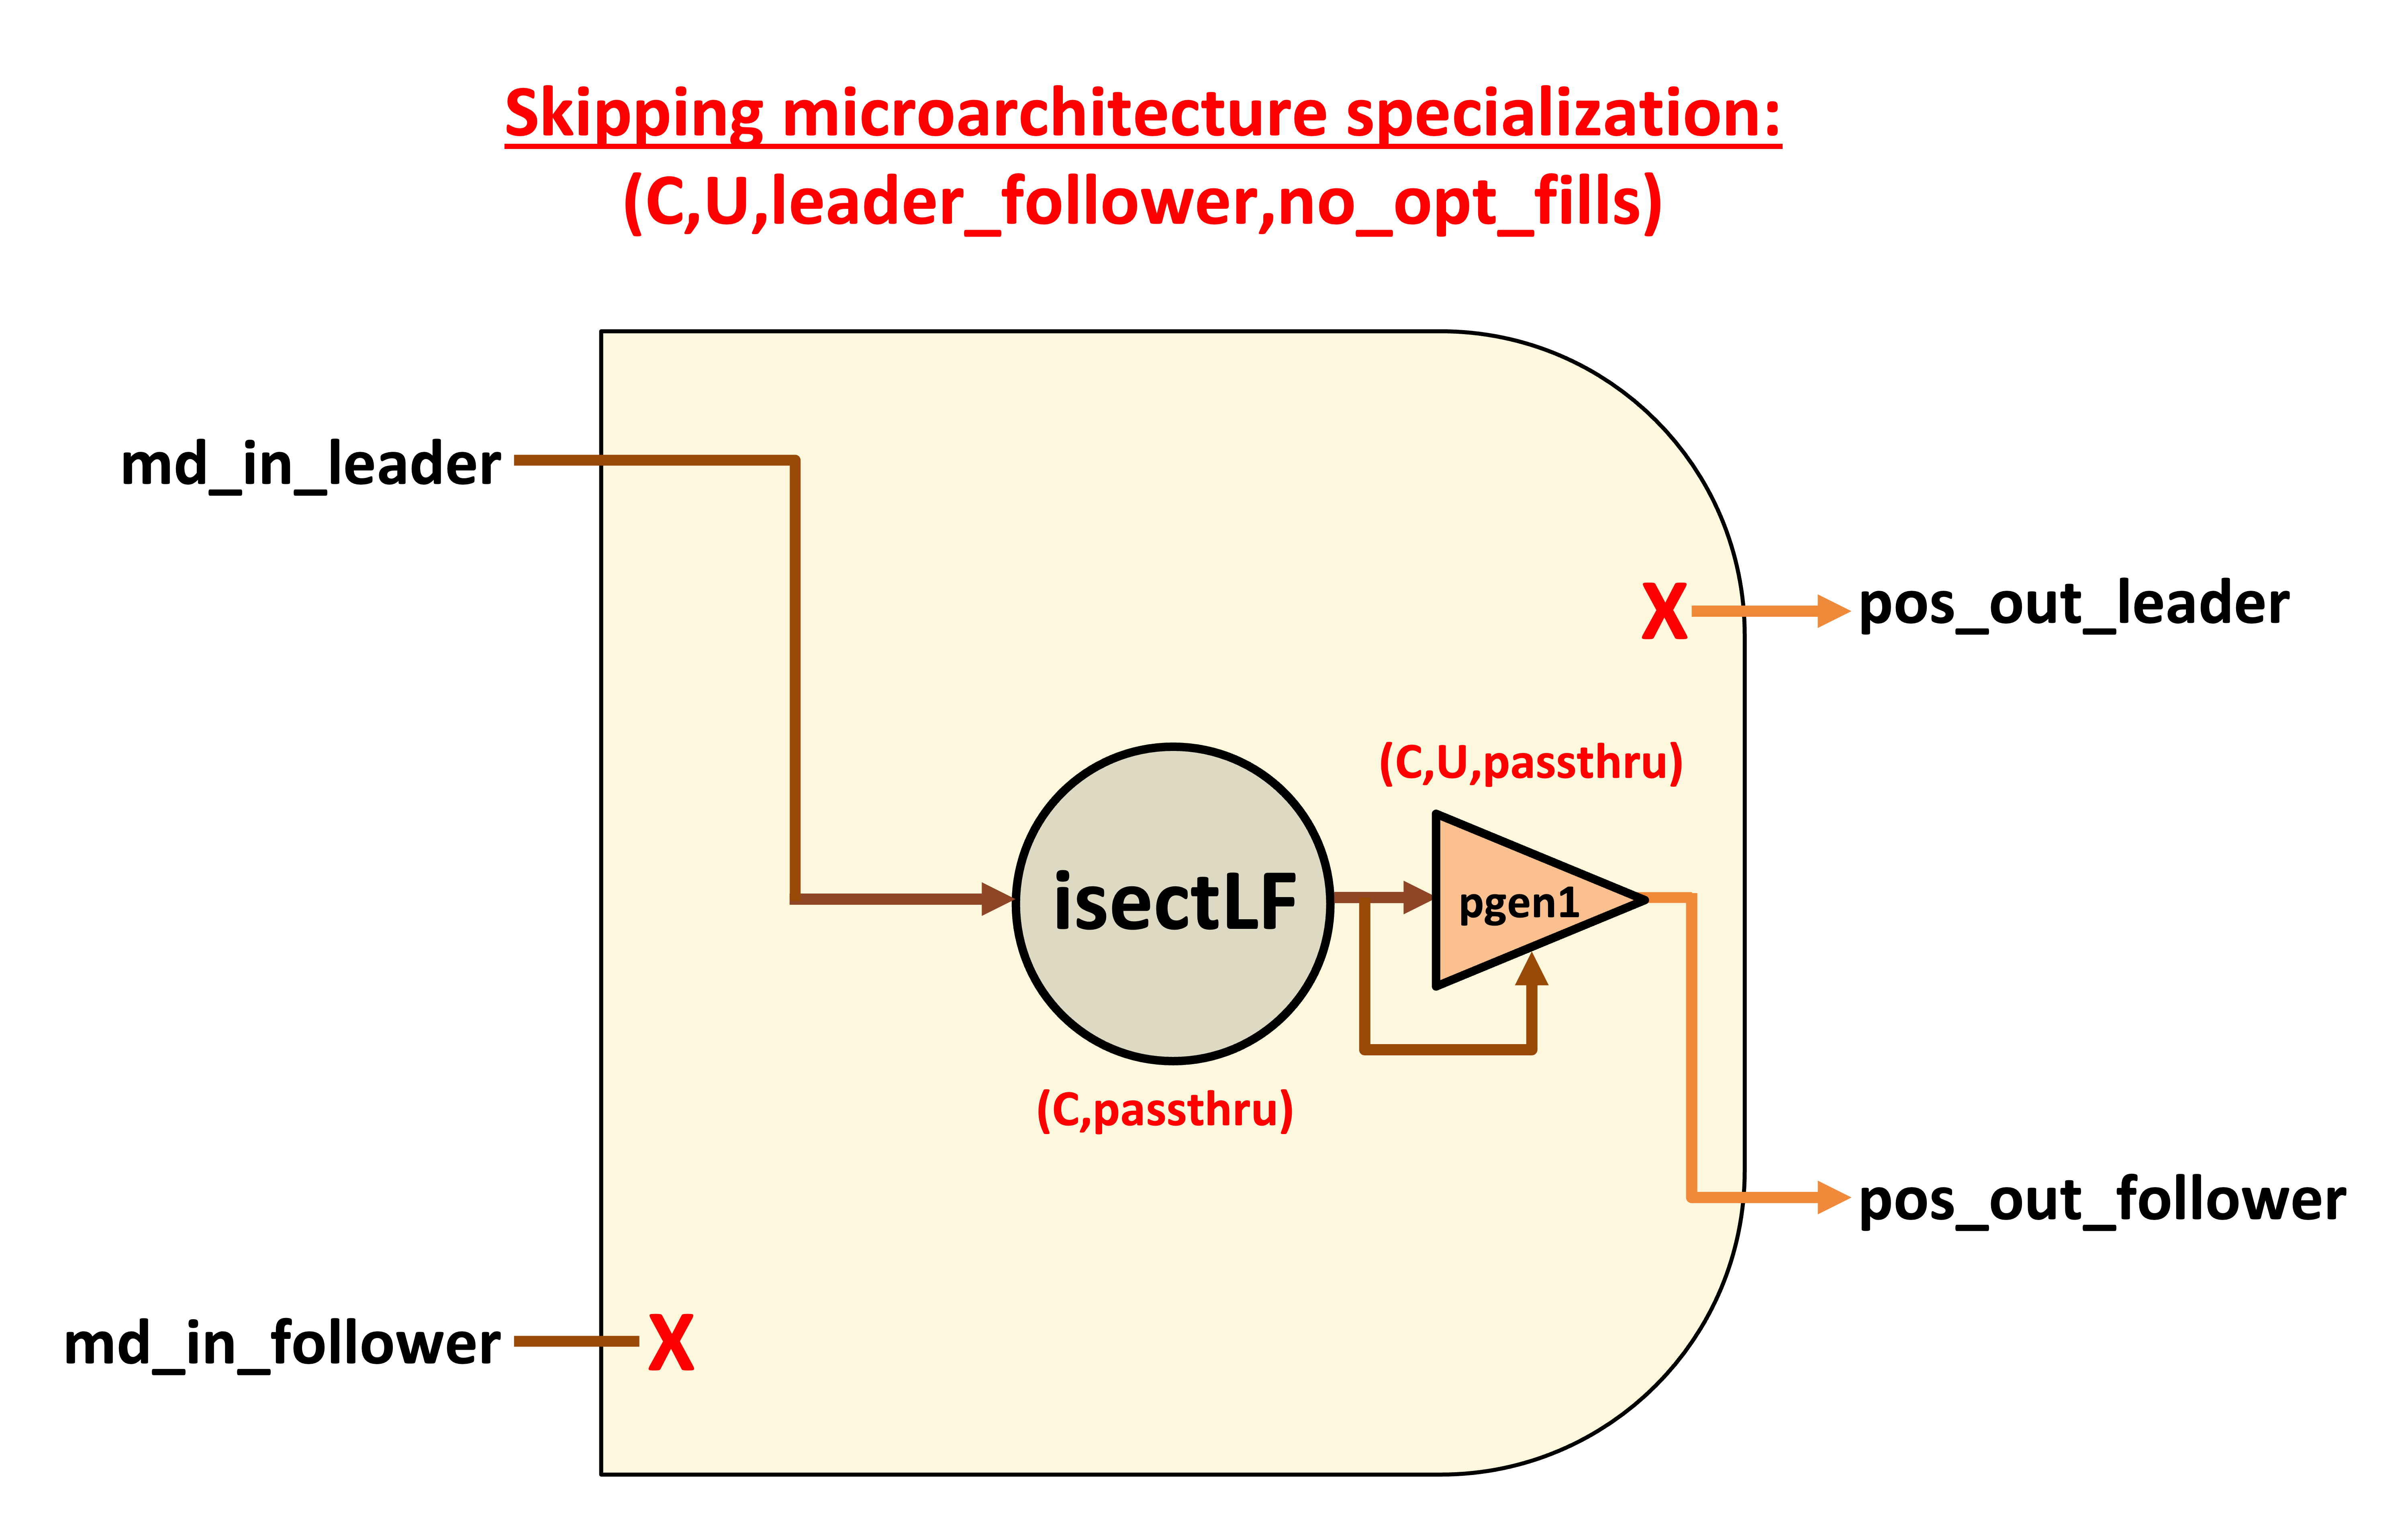
\includegraphics[width=0.95\textwidth]{figures/SKIP_C_U_leader_follower_no_opt_fills.png}
    \caption{Leader-follower coordinate-payload (C) to uncompressed offset-pair (U) skipping microarchitecture implementation topology, without fill optimization.}
    \label{fig:SKIP_C_U_leader_follower_no_opt_fills}
\end{figure}

\begin{figure}[H]
    \centering
    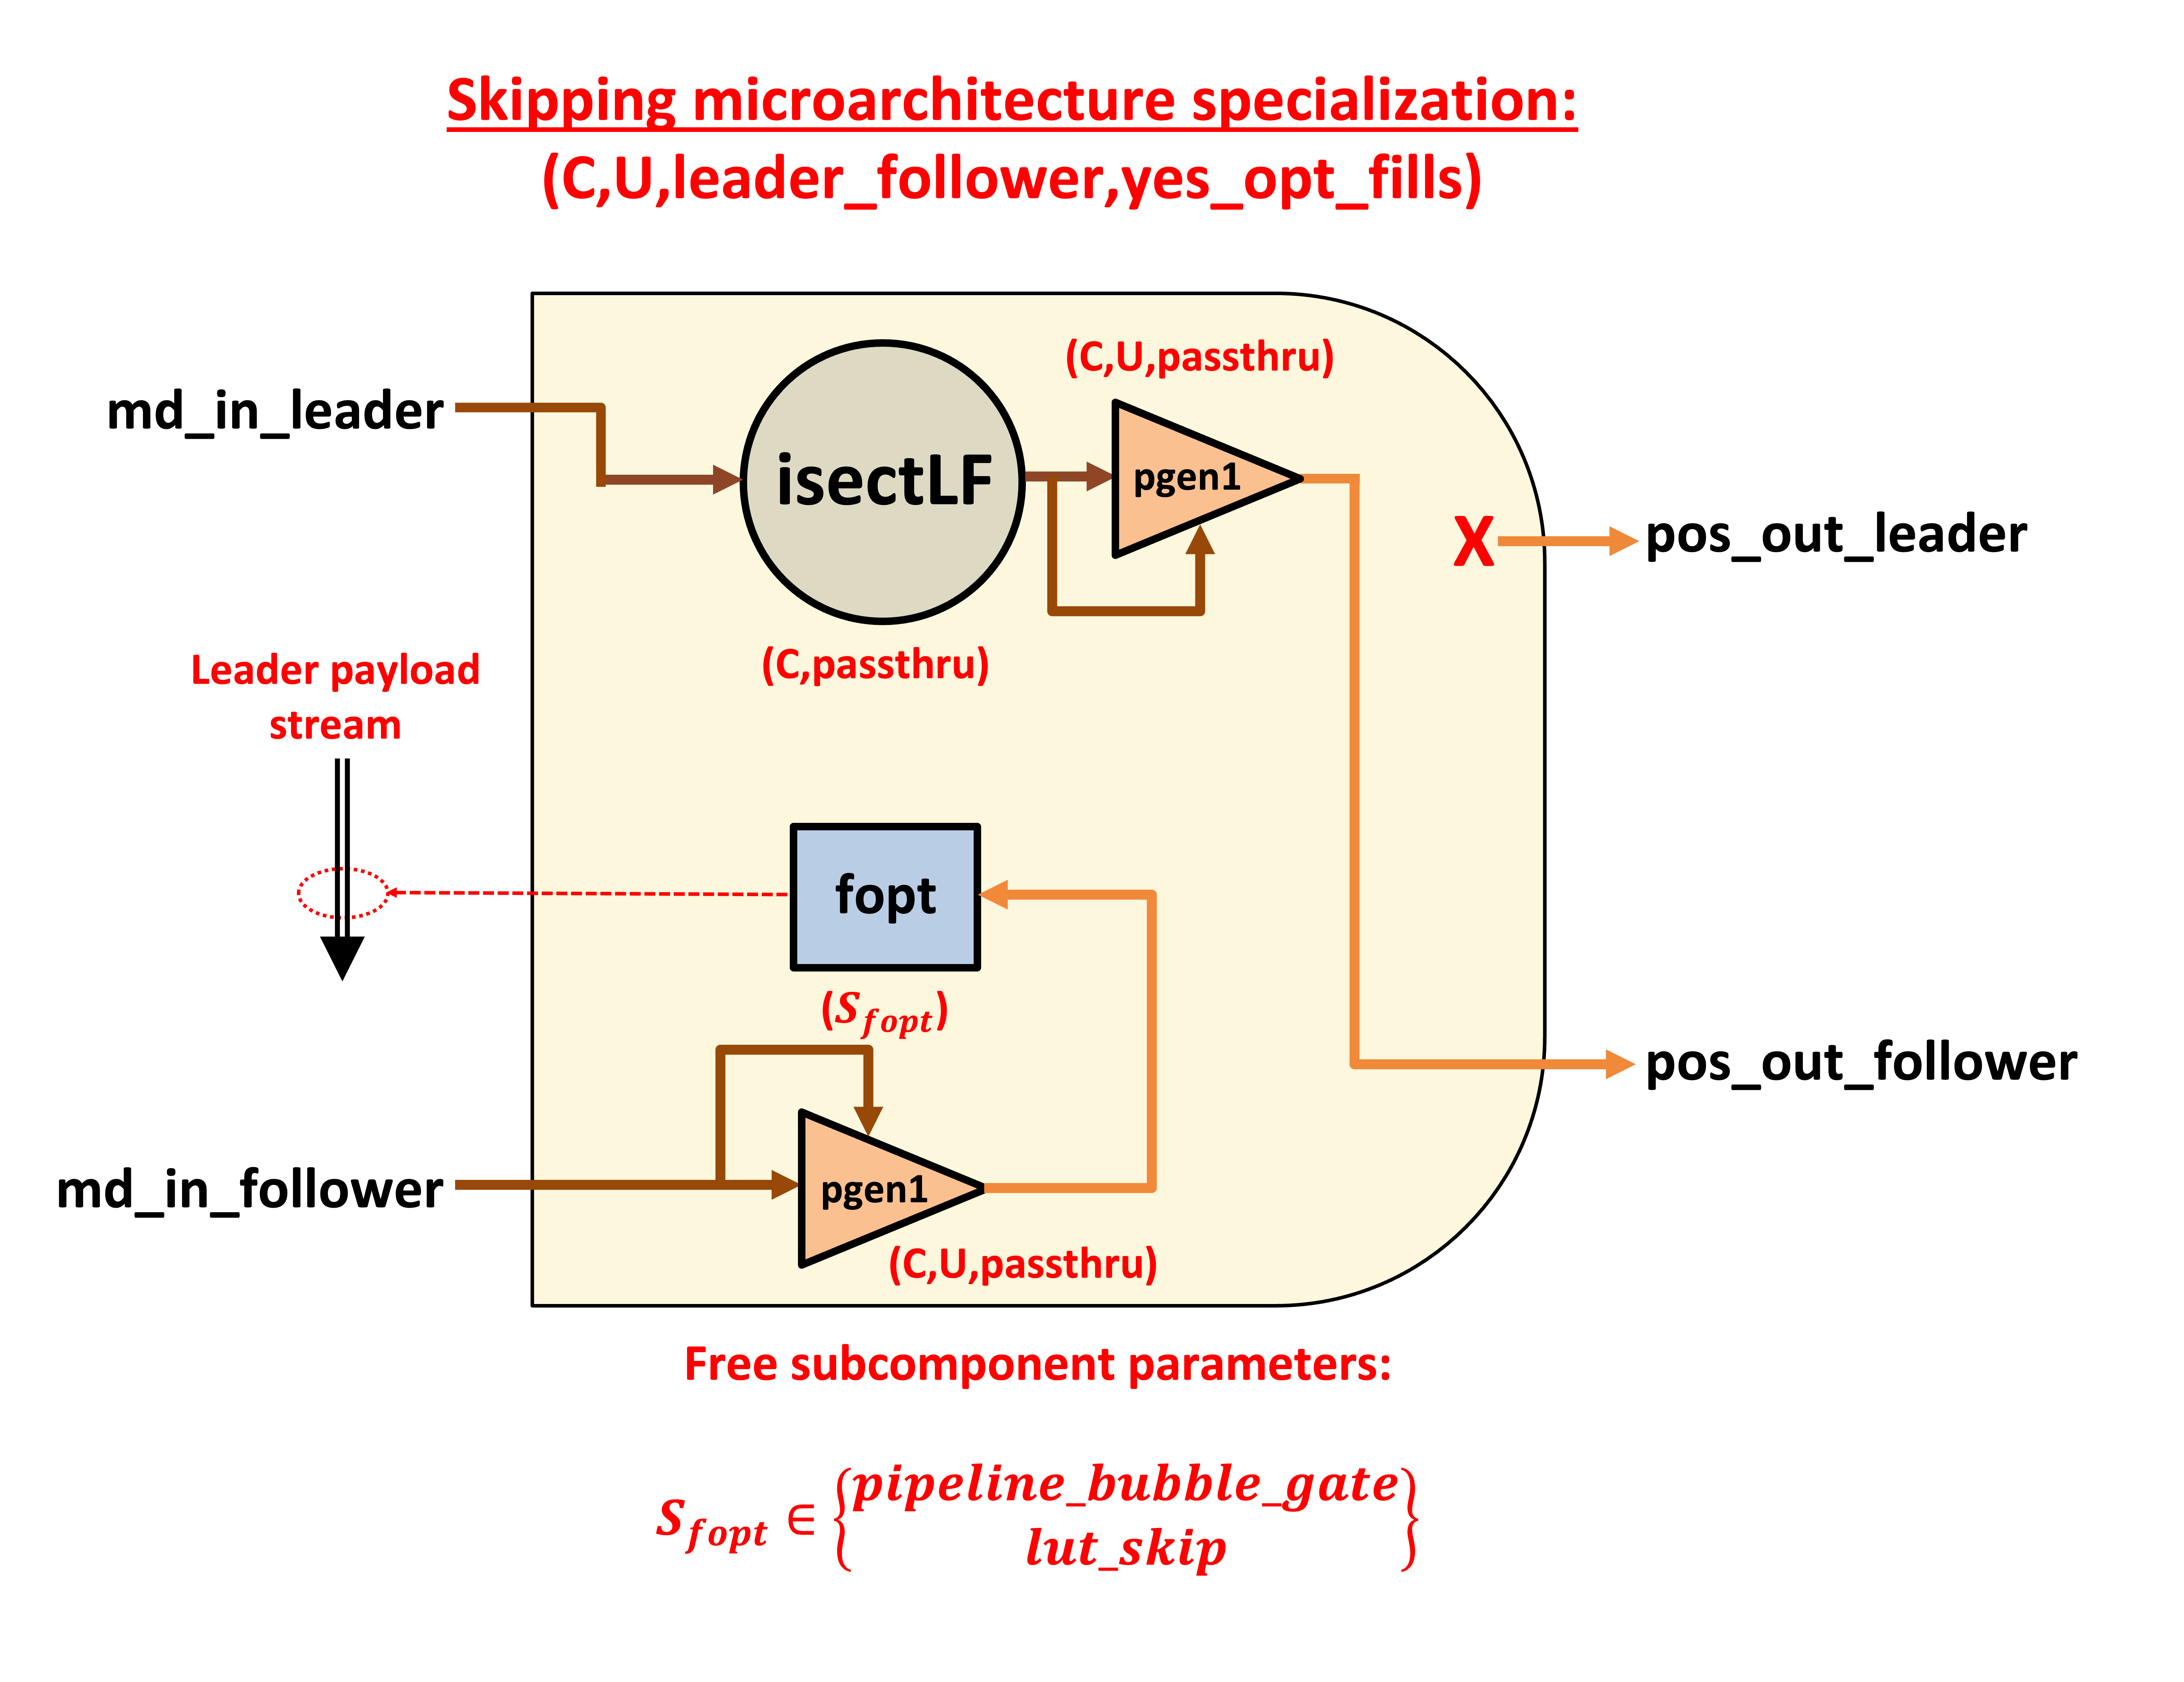
\includegraphics[width=0.95\textwidth]{figures/SKIP_C_U_leader_follower_yes_opt_fills.png}
    \caption{Leader-follower coordinate-payload (C) to uncompressed offset-pair (U) skipping microarchitecture implementation topology, with fill optimization (``Eyeriss-v2-like''\cite{eyerissv2}.)}
    \label{fig:SKIP_C_U_leader_follower_yes_opt_fills}
\end{figure}
\chapter{Challenges of design-space exploration and tradeoff comparison}

\section{Taxonomic design-space exploration of SAF microarchitectures}

\section{Utilizing SAF microarchitecture modeling for tradeoff decisions}

Taxonomic design-space exploration alone does not facilitate tradeoff decisions. A separate modeling process is required in order to compute a cost objective for comparing two or more possible microarchitecture topologies.

One challenge is that taxonomic design-space exploration yields high-level topologies but does not address low-level optimization of the microarchitecture. Ideally each SAF primitive's action-energy and area models reflect good design choices which minimize energy and area as nearly as possible; the problem is that the workload (or just ``load'') of sparse format processing work is highly dependent on where a SAF microarchitecture resides within an architecture; load-handling requirements lower-bound the cost of designing sufficiently performant SAF microarchitectures.

To that end, this section:

\begin{itemize}
    \item Develops a multi-dimensional model of the \textit{load} placed upon SAF microarchitectures
    \item Develops a conceptual framework for parameterizing SAF microarchitecture \textit{load-handling capability}
    \item Shows how to ``solve'' for energy/area models of optimized SAF microarchitectures by solving a constrained mixed-integer non-linear programming problem (MINLP). The optimization constraints are derived by applying load-modeling, circuit-modeling and composition rules to the microarchitecture topology derived from taxonomic design-space exploration
\end{itemize}

\subsection{Load modeling}

It is necessary to have an effective means of characterizing the load that is placed upon a SAF microarchitecture, as well as that component's load-handling capability. Here, load refers to the quantity of work that is imposed upon a microarchitecture, by some appropriate measure, and load-handling capability refers to the threshold load value at which a load becomes unmanageable by a particular microarchitecture. An accurate energy/area model of a microarchitecture must incorporate the insight that greater load-handling capability tends to correlate with a larger and/or more energetically costly microarchitecture\footnote{Note that while SAF microarchitecture energy-per-cycle necessarily increases when the load processed per cycle increases, the \textit{efficency} (energy-per-load-unit) may have a more complex relationship to the load-handling requirement and the microarchitecture characteristics.}.

This section describes
\begin{itemize}
\item A multi-dimensional measure of the load that architectural buffers and arithmetic units impose on SAF microarchitectures
\item A multi-dimensional measure of the load-handling capability of SAF microarchitectures
\item A process of solving for the \textit{minimum load-handling capability requirement} which each SAF microarchitecture must be designed for
\end{itemize}

The area and action-energy of each SAF microarchitecture will scale as a function of load-handling requirements; therefore, solving for minimum load-handling capability requirements is a pre-requisite for exporting analytical energy/area models.

On first blush, it might seem appropriate to use a single scalar quantity to characterize both load and load-handling capability of a component. For example, the \textit{throughput} (number of inputs processed per time) would seem like a good candidate for measuring load and load-handling requirements (since FLOPs is a common compute performance metric.)

However, it quickly becomes apparent that load and load-handling ability are multi-dimensional; what follows is a list of factors which influence loading and load-handling requirements:

\begin{itemize}
    \item \textbf{Word-width.} A microarchitecture capable of handling the throughput imposed by some workload, may nonetheless be unsuitable if i.e. the microarchitecture is expected to process sparse format metadata possessing a greater bitwidth than what the microarchitecture was designed for. Thus, word-width is a dimension of load, and the upper limit on word-width is a dimension of load-handling capability for a particular component.
    \item \textbf{Size of abstract dense rank which underlies a sparse fiber.} Consider a bitmask intersection unit, as employed in the SparTen accelerator paper \cite{sparten}. The degree of parallelism of the bitmask intersection unit microarchitecture is not a function of the throughput of metadata nor of the number of bits in a metadata word (which is in fact equal to one for bitmask format), but rather the parallelism must meet or exceed the cardinality of the abstract dense ranks which underly the sparse fibers being intersected. Thus, the cardinality of the dense rank which underlies a sparse fiber is a dimension of the load on the microarchitecture. The parallelism of the bitmask intersection unit exemplifies a dimension of the microarchitecture's load-handling capability, specifically an upper-limit on dense rank cardinality which the microarchitecture can handle.
    \item \textbf{Memory access width.} The SAF microarchitecture must be able to receive sparse format metadata in chunks equal to the memory's access bitwidth - i.e., for metadata with a bitwidth of 4 stored in a memory with 8-bit-wide reads, up to two metadata words may be made available to the SAF microarchitecture per access, worst-case. If the SAF microarchitecture only needs to read format metadata a few times over many cycles, then the latency of sequentially processing multiple metadata words can be hidden inside the time between wide reads. However, a SAF microarchitecture that is making wide memory accesses every cycle cannot hide the latency of sequential processing and thus requires a (probably more costly) SIMD design. This motivates memory access width as a dimension of load and load-handling capability.
    \item \textbf{Local architectural throughput.} Suppose that an architecture uses a SIMD MAC unit capable of 4x $C = C + A \times B$ operations per cycle to compute an inner-product; let's define $4$ MACs/cycle as the \textit{arithmetic throughput requirement.} To avoid MAC underutilization, the arithmetic throughput requirement in turn poses requirements on the whole design; for example, four $A$ and four $B$ operands per cycle are read from the $A$ and $B$ buffers respectively. 

    % Radix-2 intersection example figure
    \begin{figure}[H]
        \centering
        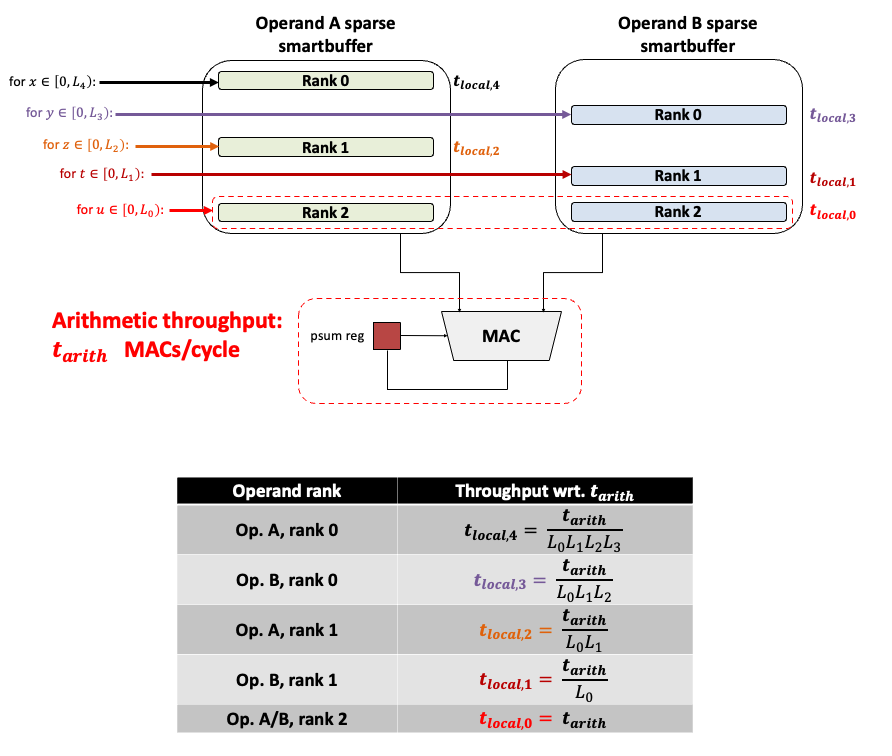
\includegraphics[width=\linewidth]{figures/local_throughput_diagram.png}
        \caption{The local throughput at each rank grows with increasing arithmetic throughput, and shrinks in proportion to the stride of the loop(s) which the fiber is bound to.}
        \label{fig:local_throughput_diagram}
    \end{figure}
    
    As an optimization, the designer implements a bidirectional skipping SAF between buffers $A$ and $B$. The skipping microarchitecture intersects $A$ and $B$ metadata and outputs a pair of $A$ and $B$ data read addresses for each intersection match. Consider what load-handling requirements the skipping microarchitecture must be designed for, in order to avoid MAC under-utilization: the skipping microarchitecture must serve $4$ $A$ addresses and $4$ $B$ addresses per cycle in order to facilitate reading 4 data values per cycle from each operand. Notably, this is a requirement on the skipping microarchitecture which results directly from the arithmetic throughput-handling design-point.

    Note that in the above example, the skipping microarchitecture, buffers, and MAC are all synchronized with the innermost loop of the mapping loop-nest; this is the fastest loop. Conversely, the outermost loops of the mapping loop-nest have greater latency between loop iterations (i.e. more cycles-per-iteration). Microarchitectures synced to slower loops can maximally exploit latency-hiding to relax throughput-handling requirements by spreading out sequential processing over the time between loop iterations. Microarchitectures synced to faster loops must be capable of handling higher processing throughput without exploiting latency hiding. This state of affairs is summarized in Figure~\ref{fig:local_throughput_diagram}
    
    As a precedent, Sparseloop\cite{sparseloop} assumes that data is pre-tiled to match the loop-nest. Under this assumption there is a reasonably clean mapping from loops in the loop nest to fibers in the fibertree of an operand, and thus a microarchitecture which interacts with fiber $i$ must support the throughput imposed by the corresponding loop in the loop-nest. For example, the inner-most loop must keep pace with the arithmetic throughput-handling requirement imposed by the MAC, so any microarchitecture which interacts with the fiber(s) corresponding to the inner loop must also keep pace with the arithmetic throughput requirement. \textit{All other things being equal}, the microarchitectural throughput-handling requirement decreases monotonically as you ascend hierarchically within a fibertree, because successively higher fibers correspond to successively slower loops. 
    
    Define \textit{local architectural throughput} as the unique throughput requirement for processing a \textit{particular} fiber within a \textit{particular} buffer, owing to the synchronization of the whole architecture with the mapping loop nest. Local architecture throughput is a key dimension of the load which the architecture imposes on a SAF microarchitecture. Consequently, throughput-handling capability is a key design requirement - \textit{but not the only key requirement} - for the SAF microarchitecture.
    
    \item \textbf{Degree of fiber sparsity.} Suppose that a fiber with a bitmask representation format resides in some buffer within an architecture. The local architecture throughput requirement for processing this fiber places a lower bound on how many non-zero fiber payloads must be traversed per cycle.

    Since it is given that the fiber is subject to a bitmask format SAF optimization, a format microarchitecture is required for parsing the metadata format. Based on the programming model developed in this work, the buffer will have several format interface ports to facilitate fiber metadata processing: \textit{md\_out}, \textit{pos\_in}, \textit{at\_bound\_in}. The format microarchitecture's ports are wired to read bitmask metadata from the buffer \textit{md\_out} port, and generate an active-high signal at \textit{at\_bound\_in} to signal when the entire fiber has been processed.

    How do we derive the format microarchitecture throughput-handling requirement from the local architectural throughput requirement associated with the fiber? The local architectural throughput applies to the rate of traversing non-zero payload values within the fiber, and the number of non-zero payloads may be much less than the dense size of the abstract rank associated with the fiber. In contrast, the number of $1$-bit bitmask metadata words matches the dense rank size regardless of how many non-zero payloads the sparse fiber has. Metadata parsing by the format microarchitecture must keep pace with the traversal of non-zero payloads in the fiber, thus if the fiber is 90\% sparse/10\% dense, $10$ $1$-bit bitmask metadata words must be parsed per non-zero data value on average; if the fiber is 99\% sparse/1\% dense, $100$ $1$-bit bitmask metadata words must be parsed per non-zero data value on average.

    More generally, for a bitmask-formatted fiber with local architectural throughput requirement $t_{arch}$ (in payloads/cycle) and a sparsity fraction $s$, the format microarchitecture must support a metadata parsing throughput of

    \[t_{parse} = \frac{1}{1-s}t_{arch}\]

    Of course, this relationship only holds for bitmask representation format. A representation format such as coordinate-payload has one explicit-coordinate metadata value per non-zero payload, thus \[t_{parse} = t_{arch}\]

    The point is, sparsity $s$ matters because it \textit{sometimes} modulates the microarchitectural throughput-handling requirement imposed by a fiber's local architectural throughput, and thus fiber sparsity is a key dimension of load.

\subsection{Loadspaces}

To concisely and effectively model loading and load-handling capability, this work builds on the concept of \textit{dataspaces} from Timeloop\cite{timeloop}.

To characterize loading, here the concept of a \textit{loadspace} is introduced. Whereas a dataspace captures the different tensor dimensions of an idealized tensor of values, a loadspace is the space of possible value for load dimensions at a particular point within an architecture or microarchitecture.

% Loadspace dimensions
\begin{figure}[H]
    \centering
    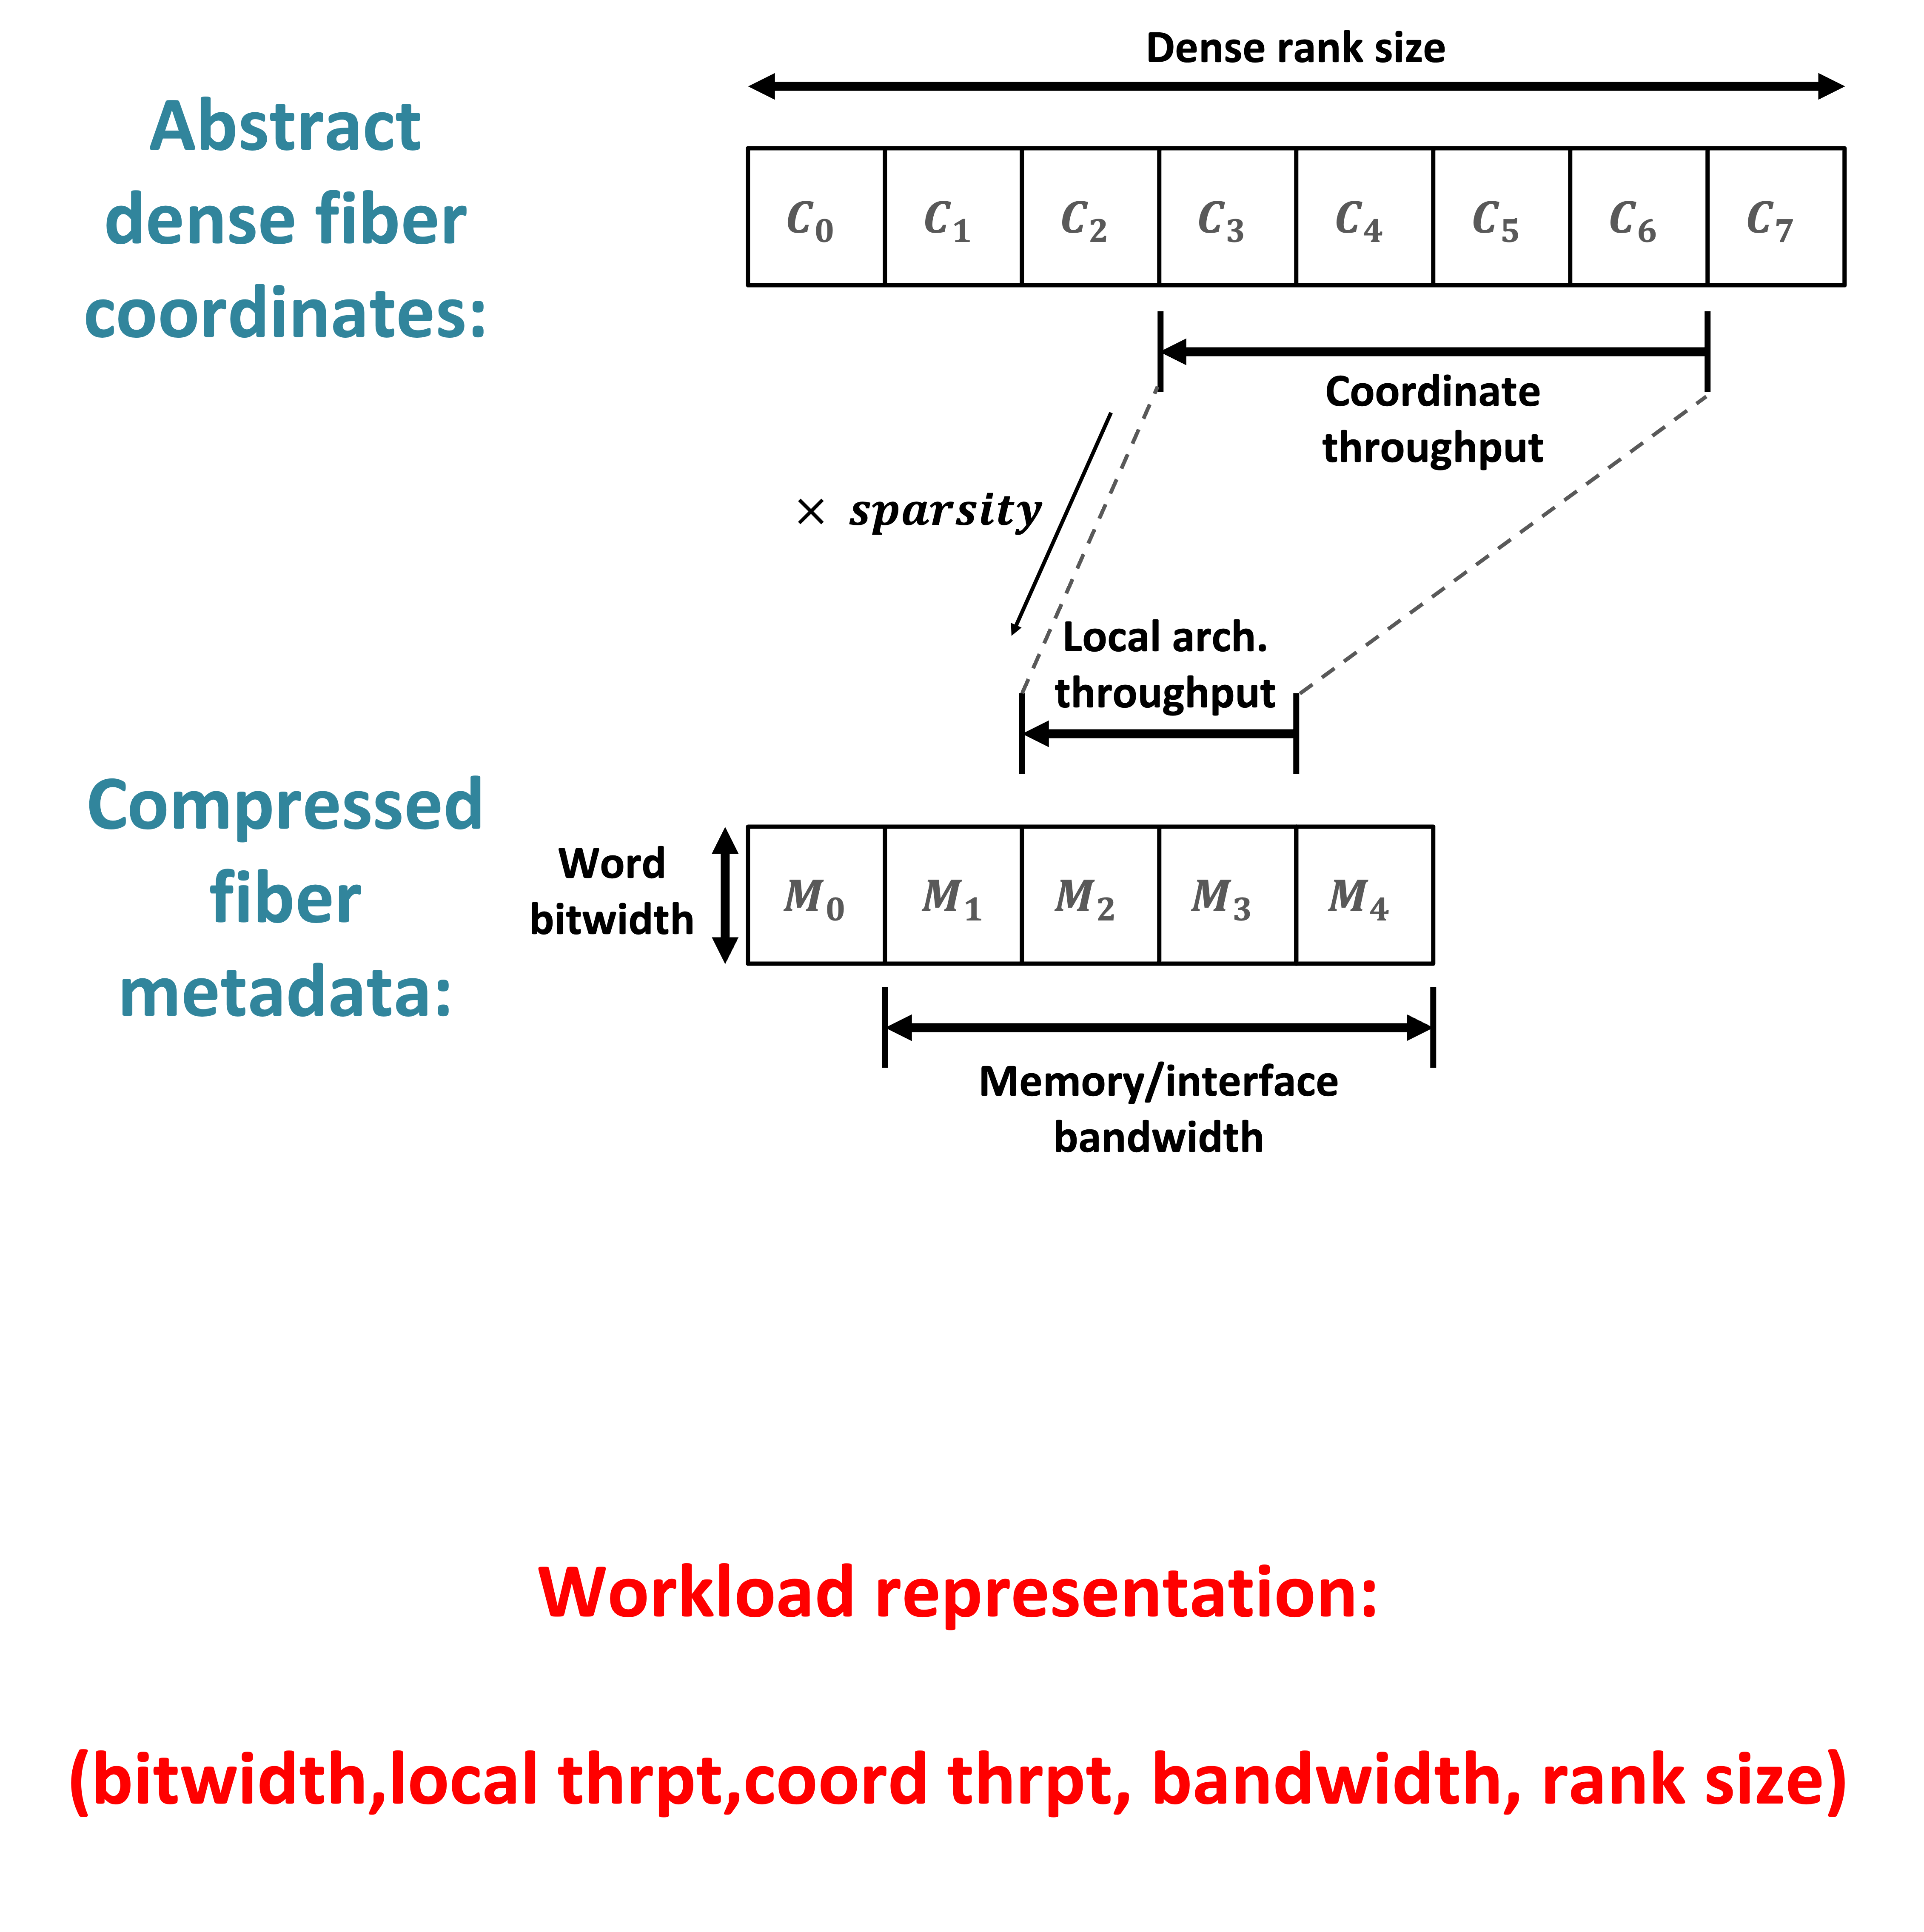
\includegraphics[width=\linewidth]{figures/workload_representation.png}
    \caption{This work proposes modeling workloads as ``loadspaces''. Here, \textit{word bitwidth},  \textit{local architectural throughput}, \textit{coordinate throughput}, and \textit{dense rank size} are proposed as key loadspace dimensions when designing SAF microarchitectures.}
    \label{fig:workload_representation}
\end{figure}

\subsection{Scalespaces}

As for modeling load handling capability, a good starting point is to note that we ultimately seek to minimize certain objective functions such as energy and area. And the modeling of these objective functions will be based on characterizing certain discrete RTL components. And these RTL components typically have a set of parameters such as data width, parallelism, etc.

Thus, analogous to load spaces, we need a way to capture the different dimensions of the load handling capability, and so we introduce scale spaces which have a dimension for each different parameter that determines the characterized energy or area of the component.

Now we can see how scale spaces and load spaces together allow us to define or solve problems in energy and area modeling. So if we consider a microarchitecture with a scale space that has two ranks and connected to a set of interfaces that collectively have a load space with two ranks,

Each point in the scale space is thus associated with a different energy area combination of values derived from characterization of the RTL .

\subsection{Deriving loadspaces from architecture and sparse optimizations}

TODO: describe how loadspaces are derived from architecture and sparse optimizations.

    \item \textbf{The meaning of ``throughput'' is representation-dependent.} This is evident in for example the coordinate metadata intersection unit described in ExTensor\cite{TODO}, in which only non-zero values are pushed onto either of the two queues leading to the intersection unit; thus, the loading on the intersection unit is a function of individual operands' sparsities. This is also evident in a microarchitectural intersection unit within a skipping microarchitecture. Its function is tied to the sparsity of both operands. An intersection requires not just a single non-zero operand but two non-zero operands simultaneously. The probability of this occurrence is a function of both operands' distribution of non-zero values. This means that sparsity, represented in whatever appropriate way, can factor into the loading on a microarchitecture.
\end{itemize}

Thus, it is clear that a single scalar value, such as throughput, is insufficient for characterizing the loading on a microarchitecture. We must resort to a multidimensional representation of loading, which therefore means that the load handling capability of a microarchitecture is also multidimensional.

Factors which impact the loading placed by an architectural port upon a SAF microarchitecture port include

\begin{itemize}
    \item \textbf{Representation formats.}
    \item \textbf{Datatypes.} SAFmodel supports three datatypes for microarchitecture ports - metadata, address, and flag. The word-width dimension of the loadspace must reflect the datatype at the applicable interface port.
\end{itemize}

\subsection{User-defined microarchitecture scale spaces}

TODO: describe how microarchitecture library must include user-specified scale-space and transfer-function descriptions.

\subsection{Continuity}

Now, consider the case of a microarchitecture with an interface that is connected to a buffer as shown in Figure~\ref{todo}.

Suppose that the microarchitecture has two scale space ranks as determined by its RTL, and the buffer interface has a load space with two ranks, perhaps indicating the sparsity and the data width.

A wire connects the interface on the buffer to the interface on the microarchitecture. So by continuity, the load space at the buffer interface is also the load space at the interface of the microarchitecture.

\subsection{Load-handling constraints}

We say that the microarchitecture can \textit{handle} the load space if for all ranks $r$ in the load space, the corresponding scale space rank $s$ satisfies $s \geq r$.

Define a point $P_L$ in the load space as an ordered pair of dimensions, where $n$ is the number of dimensions. We have a mapping $M$ that takes a load space point $P_L$ and produces a scale space point $P_S$, which is an ordered pair of scale space rank values. Let $P_{L \rightarrow S}$ represent the mapped load space point. For each dimension, it must hold that every dimension of $P_S$ is greater than or equal to the corresponding dimension of $P_{L \rightarrow S}$. Formally, if $P_S = (s_1, s_2, \ldots, s_n)$ and $P_{L \rightarrow S} = (l_1, l_2, \ldots, l_n)$, then for each $i$, $s_i \geq l_i$.

In other words, the projection of the load space point into scale space must lie within the feasible region defined by the scale space inequality.

\subsection{Circuits}

TODO: talk about daisy-chaining

\subsection{Component composition}

Now, one challenge in defining primitive components is that often they're comprised of more than one RTL block, and so we need a way to define scale space for an entire primitive component that is built out of multiple RTL blocks.

To do this, we can define a scale space for the whole component and then take note of what are the individual scale spaces of the RTL blocks comprising the components, and then based on an intuition about how the larger component interacts with the sub-components, we can define a set of mappings from the scale space of the whole component to the scale spaces of each of its RTL blocks.

Returning to the previous example where we had a component connected by a wire to a buffer and we defined an inequality relating the component scale space to the load scale space and we said that the load space projection into scale space must fall within the feasible region of the inequality. Now what we can do is use the mappings from the component scale space to the RTL scale spaces in order to project the inequality onto the RTL scale spaces and this then allows us to define inequalities between the RTL scale spaces and the load space terms of the buffer.

\subsection{Building an MINLP optimization problem}

Applying this process to the topology of an entire architecture, we are able to obtain a large set of inequalities which define the feasible regions for all of the RTL blocks comprising all of the microarchitectural components. And then we can set up a mixed-integer nonlinear program problem which tries to simultaneously solve for a set of all load spaces that is compatible with some assignment of scale space points to all components. The solution to this problem allows us to determine the scaling of all microarchitecture components in the design.
\chapter{SAFtools framework}


\chapter{Evaluation}
\label{chapter:evaluation}

\section{Methodology}

\todo{Describe validation and evaluation process}

%\subsection{Simulation Speed}

\section{Validation}

\todo{Model PE experiment} 
\chapter{Case study}
\label{chapter:case_studies}

This case-study explores the tradeoff of different skipping microarchitectures in a scenario where the sparse tensor accelerator exploits a SIMD MAC.

\section{Methodology}

 Here one case study is provided which showcases

\begin{itemize}
    \item SAF microarchitecture taxonomic inference with SAFinfer.
    \item SAF microarchitecture scale inference with SAFmodel.
    \item Tradeoff study comparing different choices of coordinate-payload intersection unit.
\end{itemize}

SAFmodel was also used to generate Accelergy analytical models for use with Sparseloop; however, for a variety of reasons, these models were not integrated into a Sparseloop testbench; the tradeoff study here only compares the energy-per-action and area overhead of SAF microarchitectures but does not use Sparseloop to obtain action counts or get energy/area estimates for the rest of the architecture.

SAFTools allows the user to customize the objective function for optimizing SAF microarchitecture. In this work, the objective function is the total energy-per-action/area product, over all SAF microarchitecture primitives and all actions. This is the default SAFTools objective function, and it is chosen in order to co-optimize energy and area. 

\begin{figure}[ht]
\centering
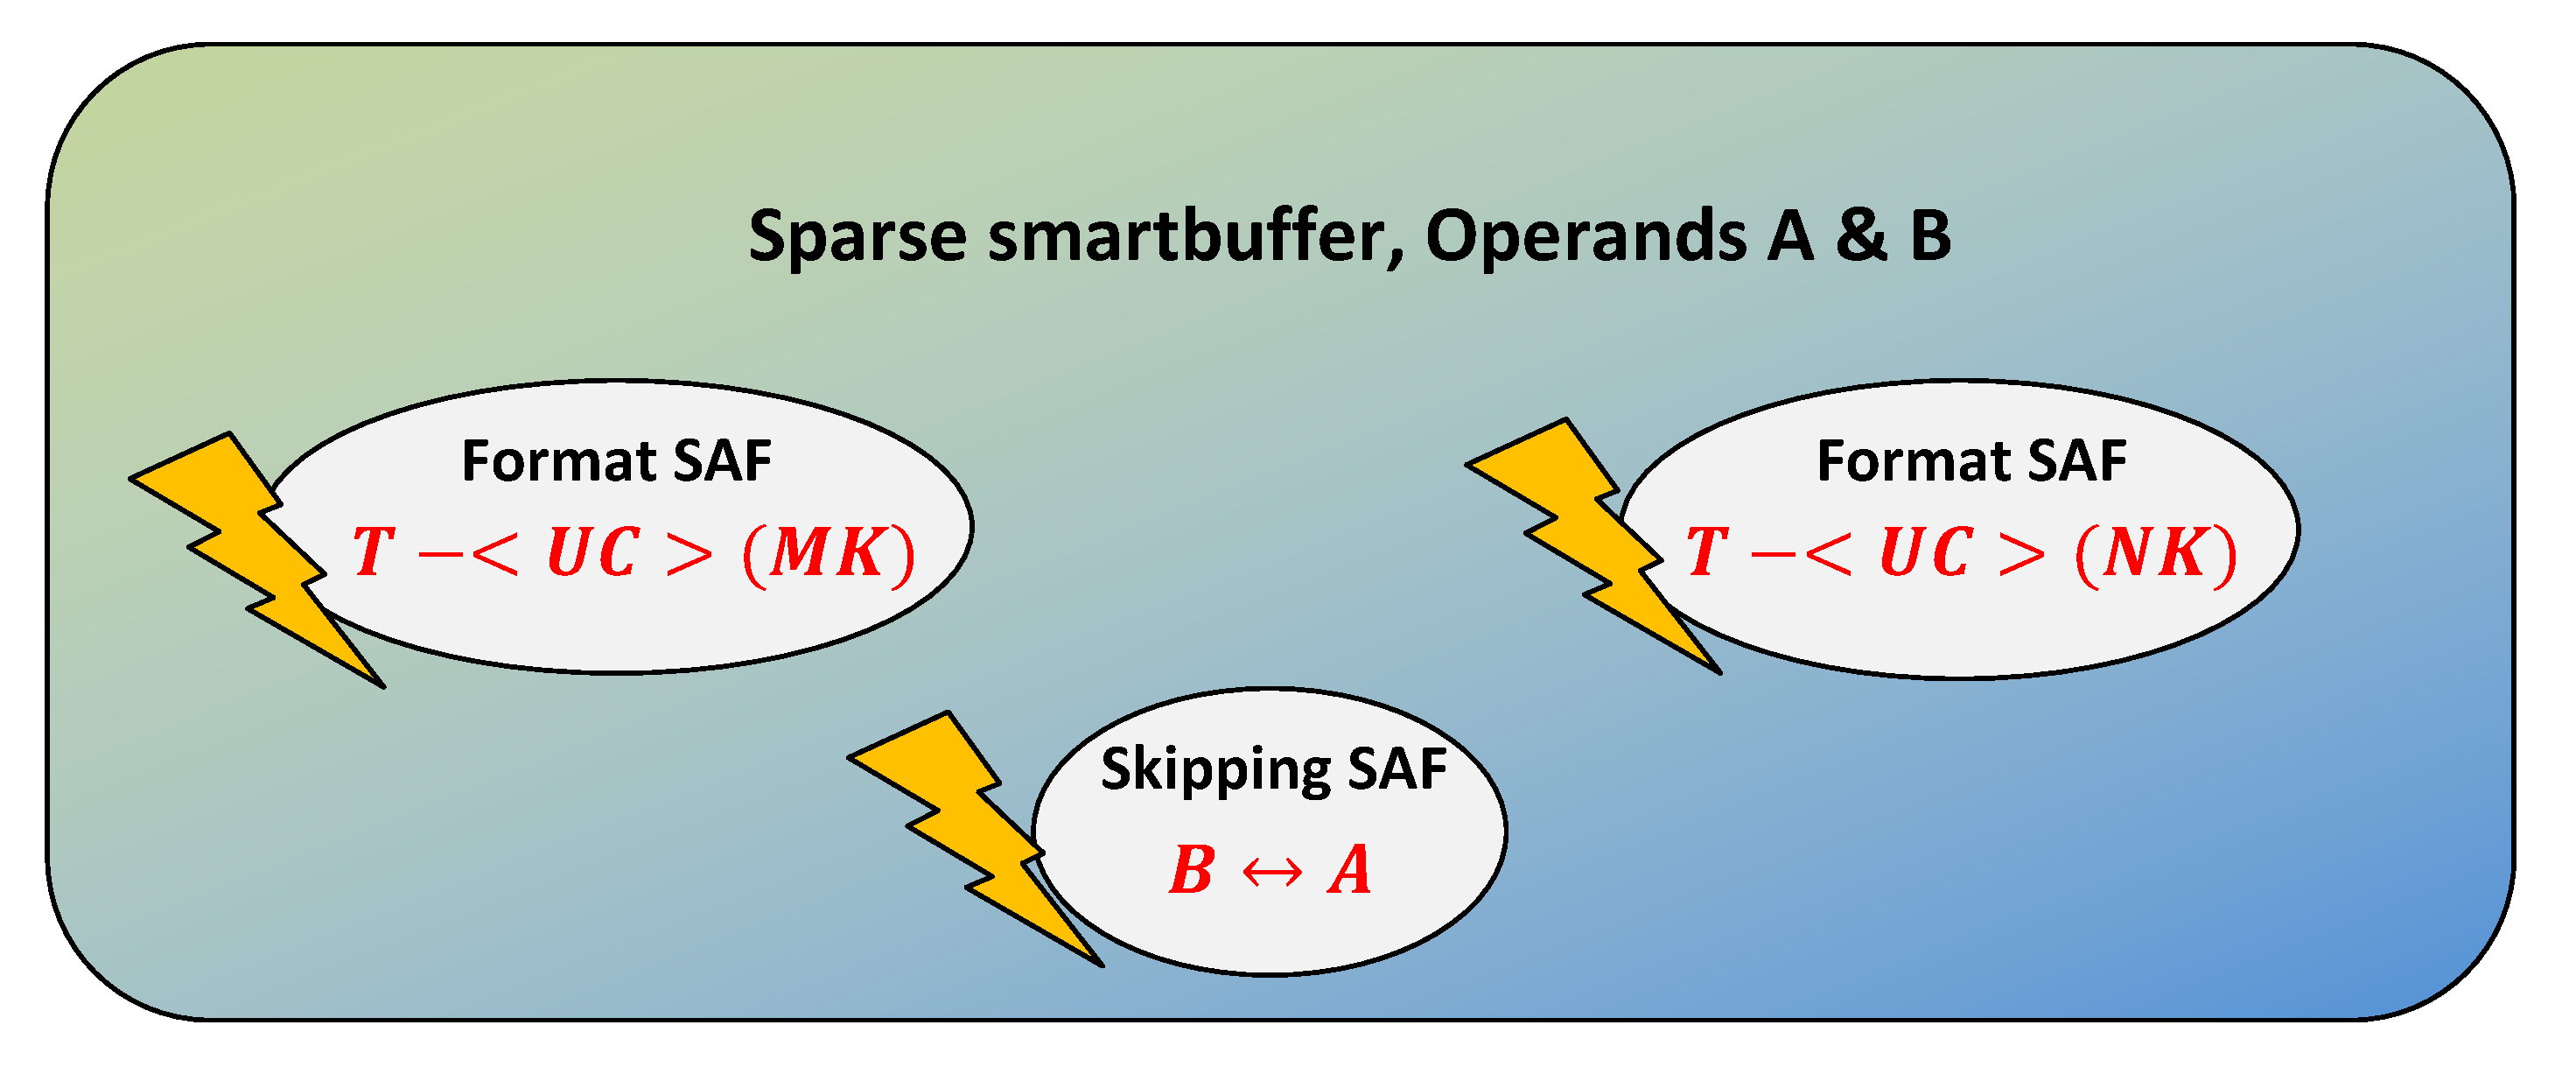
\includegraphics[width=0.85\textwidth]{figures/case_study_declarative.pdf}
\caption{Sparseloop configuration files provided to SAFinfer.}
\label{fig:case_study_declarative}
\end{figure}

For taxonomic inference, SAFinfer was provided Sparseloop configuration files specifying a hypothetical architecture with a buffer holding both input operands resident, both in CSR format (T-<UC>(MK) and T-<UC>(NK) respectively), and subject to a bidirectional skipping SAF. This state of affairs is summarized in Figure~\ref{fig:case_study_declarative}. This Sparseloop configuration file is meant to represent spGEMM without tiling\footnote{SAFinfer only consumes the Sparseloop architecture and Sparseopts files; SAFinfer does not have access to the problem einsum or mapping\cite{sparseloop}.} Additionally there is a single partial sum register for accumulating the inner product in a dense/uncompressed format.

For scale inference, SAFmodel was provided the SAFinfer output microarchitecture as well as a requirement to use energy-per-action/area product as the objective function to minimize during scale inference. SAFmodel was instrumented to output a sweep over valid scale parameter configurations $\{S_x\}_{valid}$, for the purposes of visualizing and comparing possible combinations of low-level scale parameters such as input vectorization, pipeline depth, etc.

Designs such as Eyeriss v2\cite{eyerissv2} exploit SIMD MAC units in order to accelerate processing, however this places increased pressure on the rest of the design to support doubled throughput. This observation suggested an opportunity to explore the impact of throughput requirements on scale inference in skipping microarchitectures.

\section{Results}

\subsection{Inferred SAF microarchitecture}

\begin{figure}[ht]
\centering
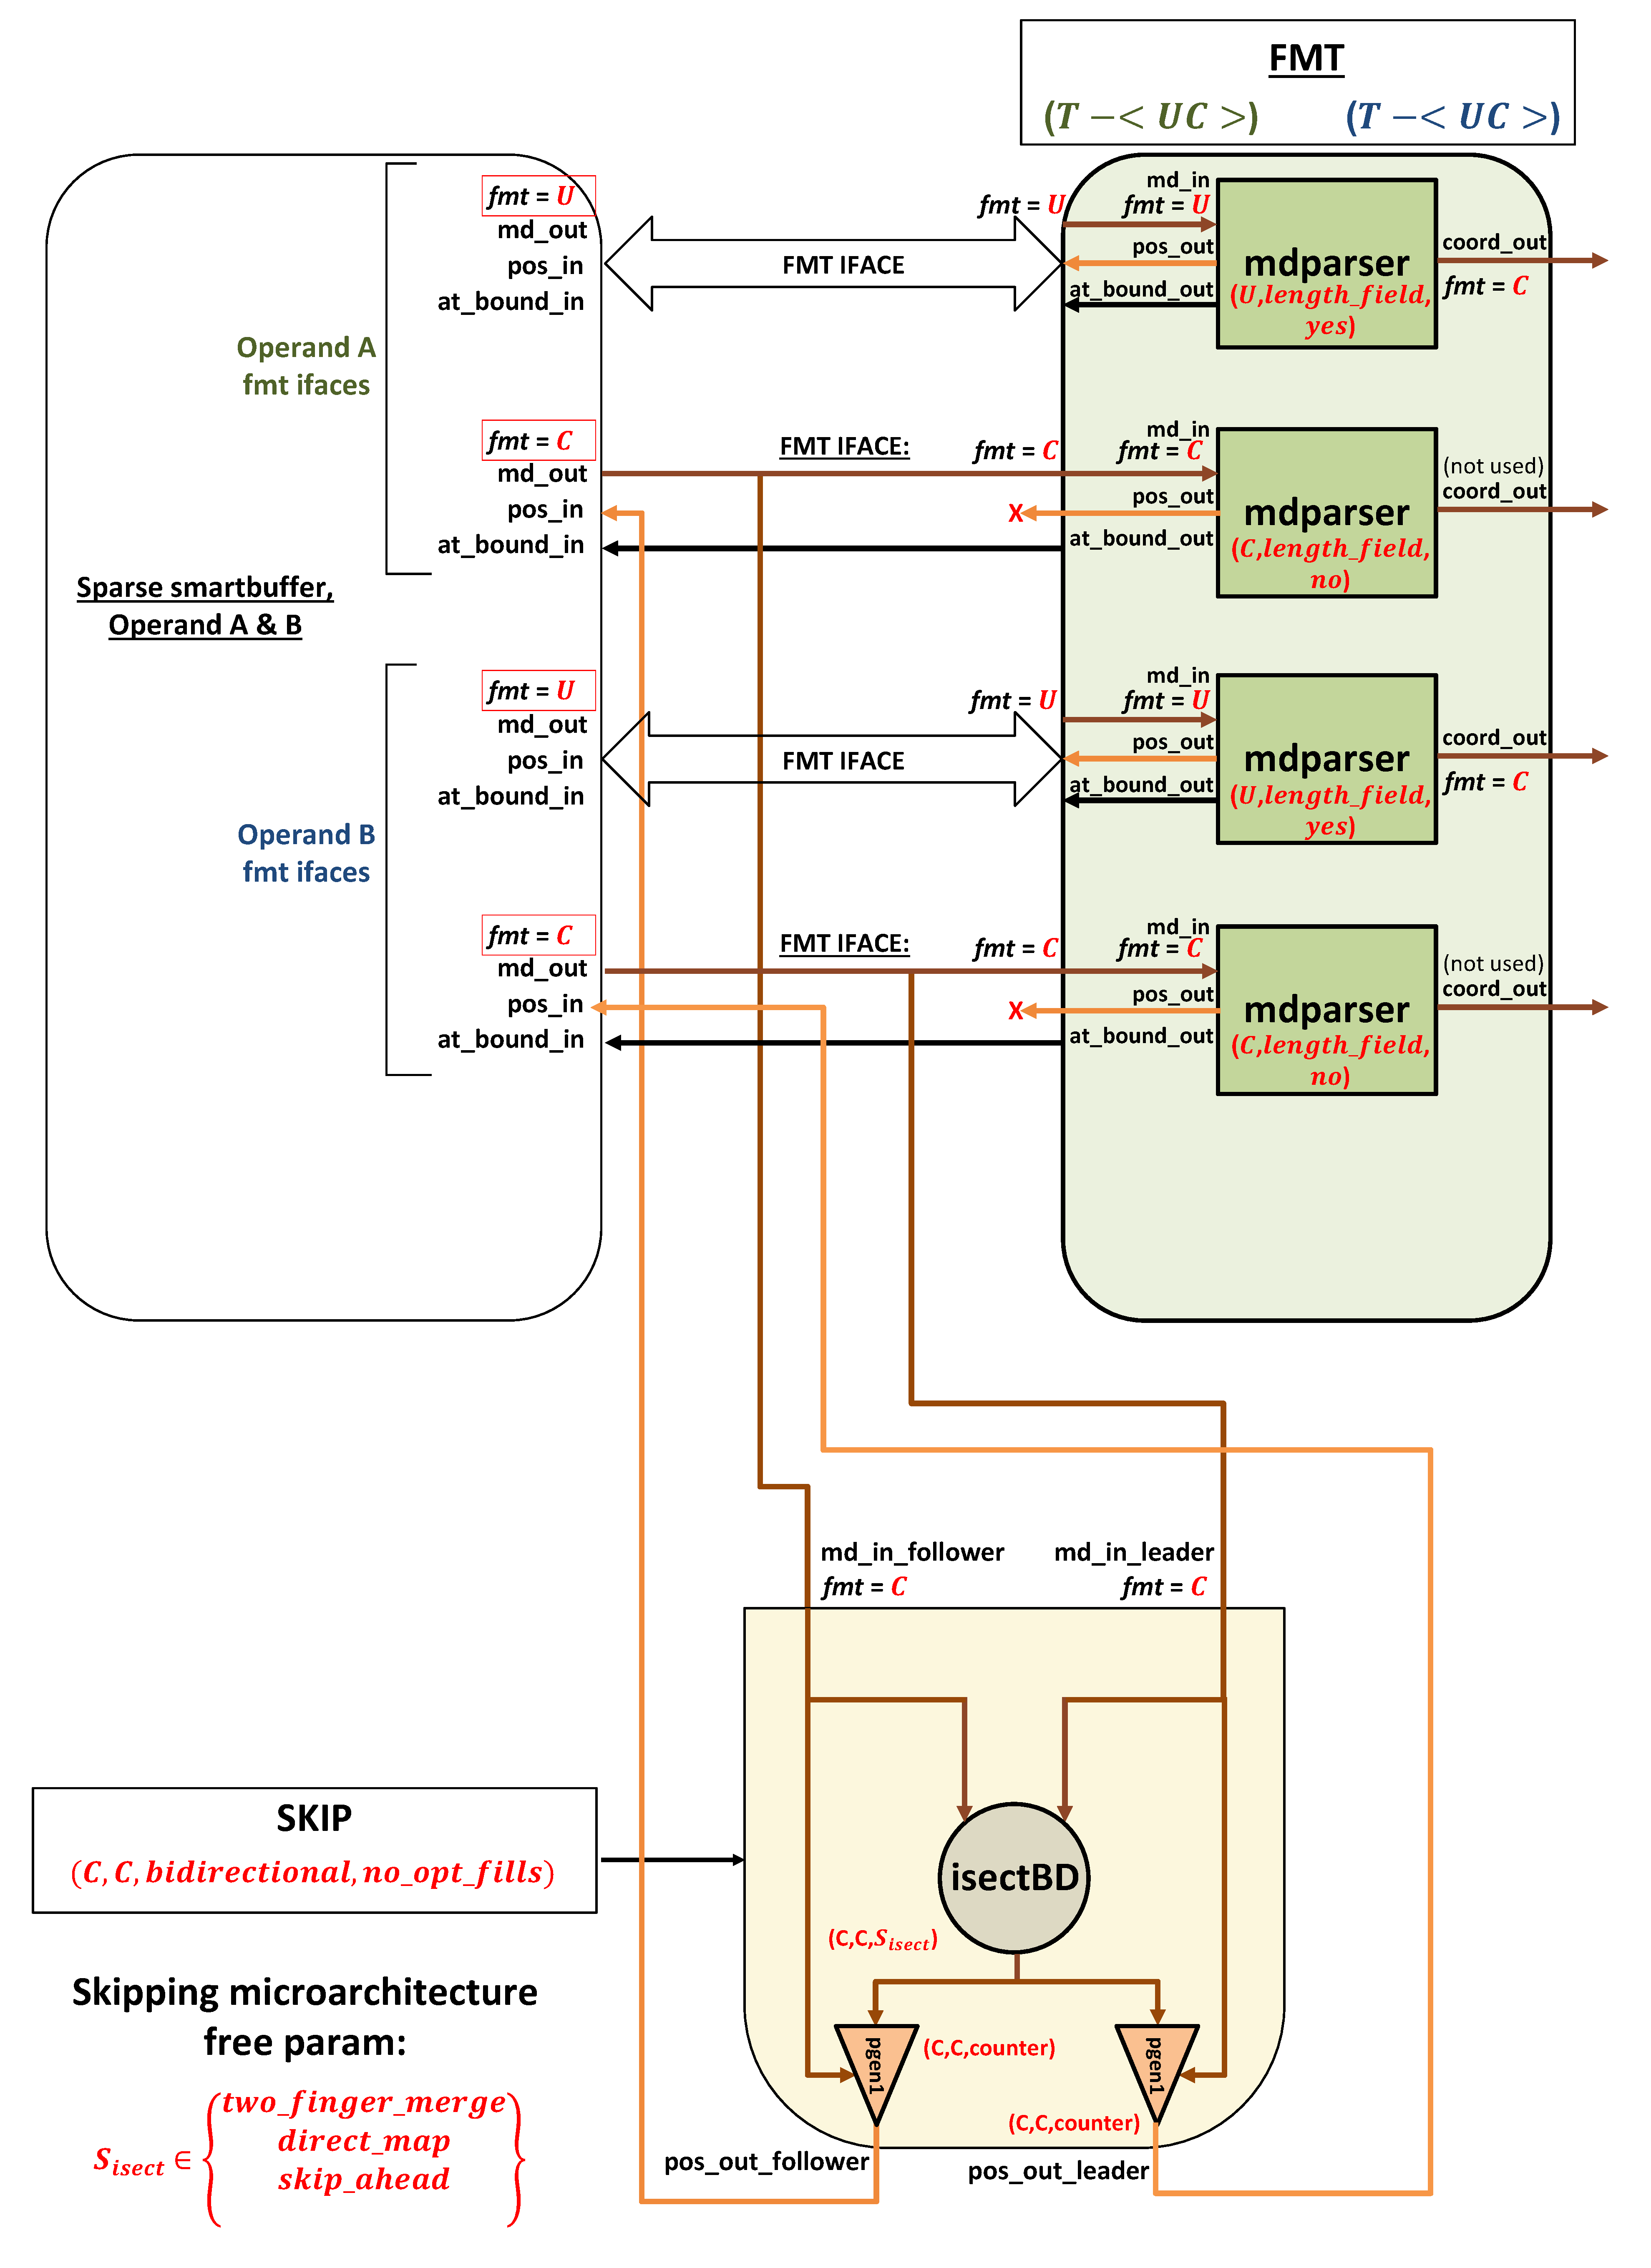
\includegraphics[width=0.7\textwidth]{figures/case_study_inferred_uarch.pdf}
\caption{SAF microarchitecture synthesized by SAFinfer based on declarative specifications.}
\label{fig:case_study_inferred_uarch}
\end{figure}

\clearpage

Figure~\ref{fig:case_study_inferred_uarch} shows the SAF microarchitecture inferred by SAFinfer based on the declarative specifications in the Sparseloop config file. The SAF microarchitecture comprises

\begin{itemize}
    \item A format microarchitecture containing four metadata parsers, one for each rank of each operand fibertree.
    \item A skipping microarchitecture with attributes $(C,C,bidirectional,no\_opt\_fills)$, wired to the format interfaces associated with the two coordinate-payload-format fibers. The skipping microarchitecture comprises a bidirectional intersection unit, as well as two pgen1 units each with attributes $(C,C,counter)$.
\end{itemize}

The bidirectional intersection unit within the skipping microarchitecture has attributes $(C,C,S_{isect})$ where $S_{isect}$ is a free parameter which may be chosen by the user to be either $two\_finger\_merge$ (i.e. ExTensor-like\cite{extensor} naive two-finger merge-like intersection), $direct\_map$ (the direct-mapped intersection unit developed in this work), or $skip\_ahead$ (i.e. ExTensor-like optimized intersection.)

Note that both pgen1 units in the skipping microarchitecture are wired to the format interface pos\_in inputs on the sparse smartbuffer; thus, the output throughput from each pgen1 unit must be be greater-than-or-equal-to the boundary throughput requirement at the corresponding pos\_in inputs, which in turn is a function of the arithmetic throughput as well as the loop nest stride. Thus, as part of an experiment, we can adjust the boundary throughput requirement at pos\_in to reflect what would be required for SIMD 2 arithmetic; SAFmodel scale inference will automatically optimize the skipping microarchitecture to support the necessary throughput.

\subsection{Analysis: skipping microarchitecture design tradeoffs}

\begin{figure}[H]
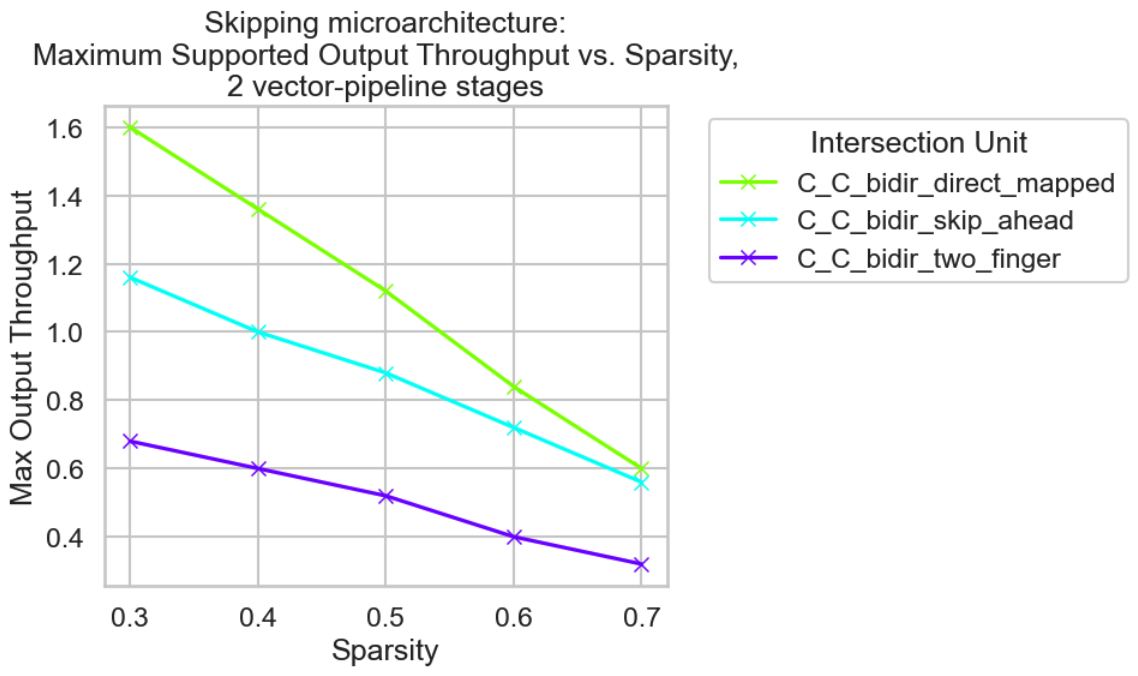
\includegraphics[width=\textwidth]{figures/skip_uarch_pipe_2.png}
\caption{Analysis of intersection unit transfer relations: peak match throughput vs operand sparsity, for intersection units units with two pipeline stages.}
\label{fig:skip_uarch_pipe_2}
\end{figure}

\begin{figure}[H]
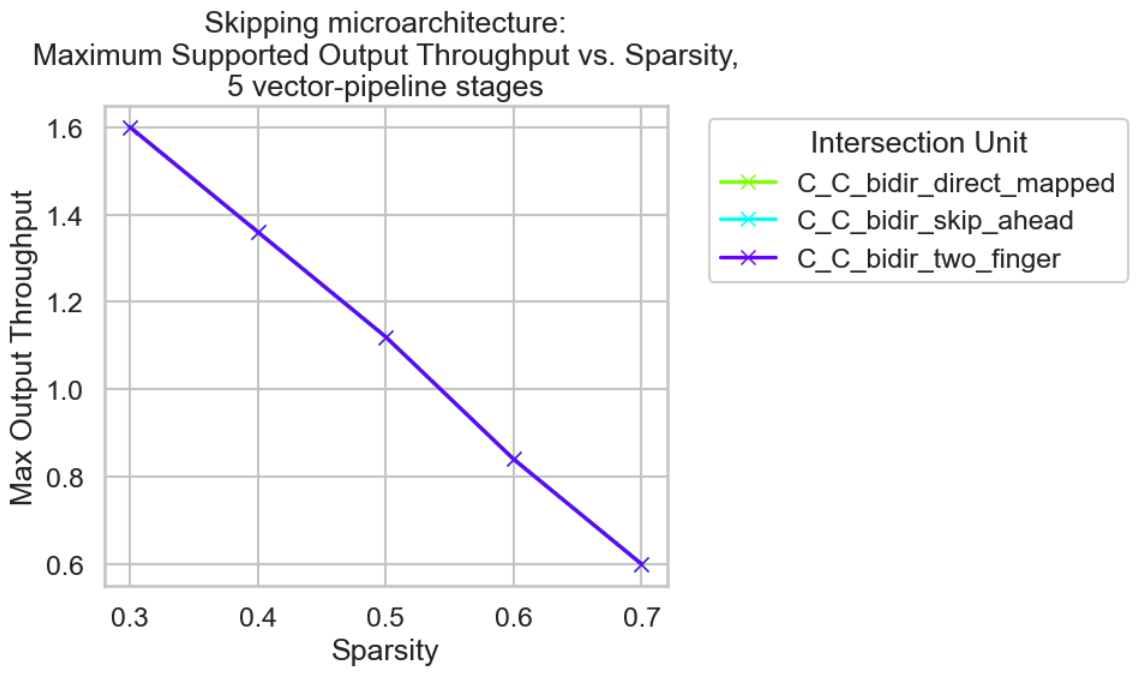
\includegraphics[width=\textwidth]{figures/skip_uarch_pipe_5.png}
\caption{Analysis of intersection unit transfer relations: peak match throughput vs operand sparsity, for intersection units units with five pipeline stages.}
\label{fig:skip_uarch_pipe_5}
\end{figure}

Figures~\ref{fig:skip_uarch_pipe_2} and~\ref{fig:skip_uarch_pipe_5} compare the throughput at the output of the pgen1 units, to the sparsity of the intersection unit input fiber operands, compared between all three intersection unit types for a dense fiber rank size of 16 and a degree-of-vectorization of 4. Figure~\ref{fig:skip_uarch_pipe_2} considers intersection units with 2 pipeline stages while Figure~\ref{fig:skip_uarch_pipe_5} considers intersection units with 5 pipeline stages. 

Note that the relationship between max throughput and sparsity is derived from the transfer relation model that was developed in Section~\ref{sec:c_c_isect_modeling}.

It is clear that pipelining is key to supporting high-throughput intersection, which in turn is critical in a SIMD scenario. It is worth noting that in the scenario shown (vectorization 4, rank size 16), none of these intersection units could supply 2 matches/cycle to support a SIMD 2 arithmetic unit; the max is 1.6 matches/cycle regardless of pipelining. More detailed analysis of the peak matches/cycle throughput supported by each intersection unit variety is provided in Appendix~\ref{appendix:app_intersection_modeling}.

In Figure~\ref{fig:skip_uarch_pipe_2}, direct-mapped intersection attains the highest throughput, followed by skip-ahead intersection unit; this makes sense since direct-mapped intersection has 100\% pipeline efficiency and skip-ahead intersection unit has optimizations to increase pipeline efficiency. This also shows that with 2 pipeline stages, the intersection unit is \textit{efficiency-limited} i.e. limited by how efficient the choice of intersection unit is when it comes to maximizing the number of matches found by a pipeline stage per cycle.

In contrast, in Figure~\ref{fig:skip_uarch_pipe_5}, all intersection units are capable of attaining the same throughput with 5 pipeline stages; this shows that with enough pipeline stages, the intersection unit is \textit{input-rate-limited}, i.e. it is not possible to output more intersections per cycle without changing fiber sparsity, dense rank size, or input vectorization of the intersection unit. Being input-rate-limited is broadly speaking a ``good'' thing, since it means that the particular type of intersection unit we chose is not slowing down the design. We can further observe that while two-finger and skip-ahead intersection unit required multiple pipeline stages in order to be input-rate-limited, direct-mapped intersection unit is already input-rate-limited in Figure~\ref{fig:skip_uarch_pipe_2}. This is because by design, direct-mapped intersection finds all matches in a single cycle, and thus requires only one pipeline stage.

\begin{figure}[H]
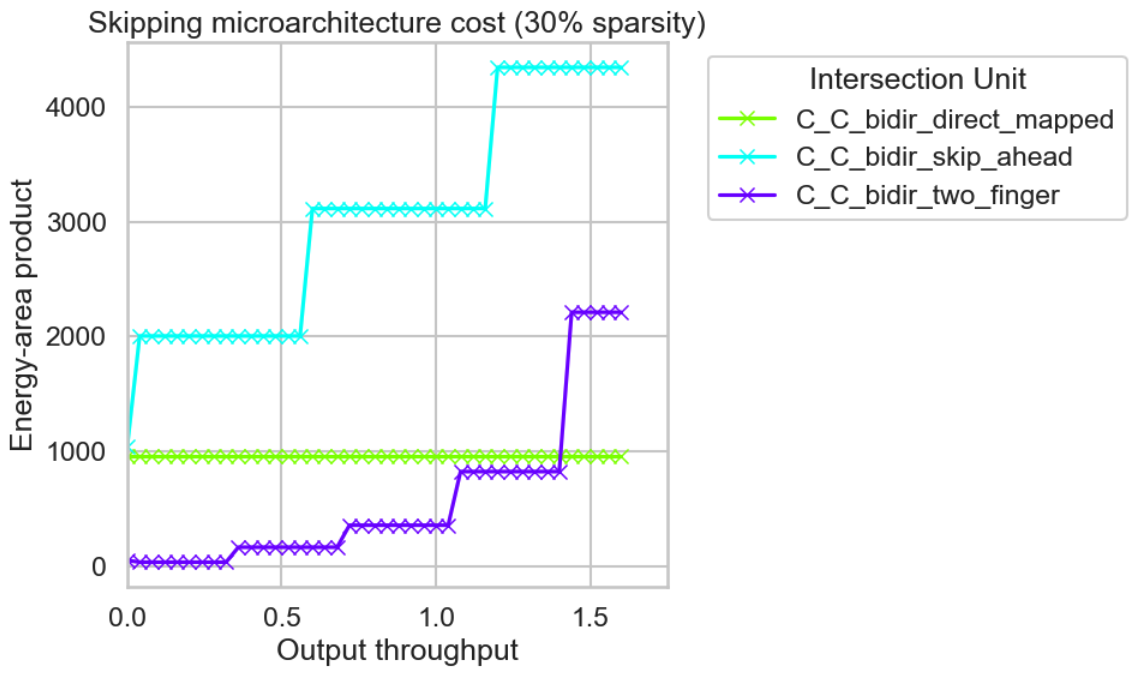
\includegraphics[width=\textwidth]{figures/skip_uarch_sparsity_30pct.png}
\caption{Comparison of energy-per-action/area product for 30\% sparse operands over a range of output throughput requirements.}
\label{fig:skip_uarch_sparsity_30pct}
\end{figure}

\begin{figure}[H]
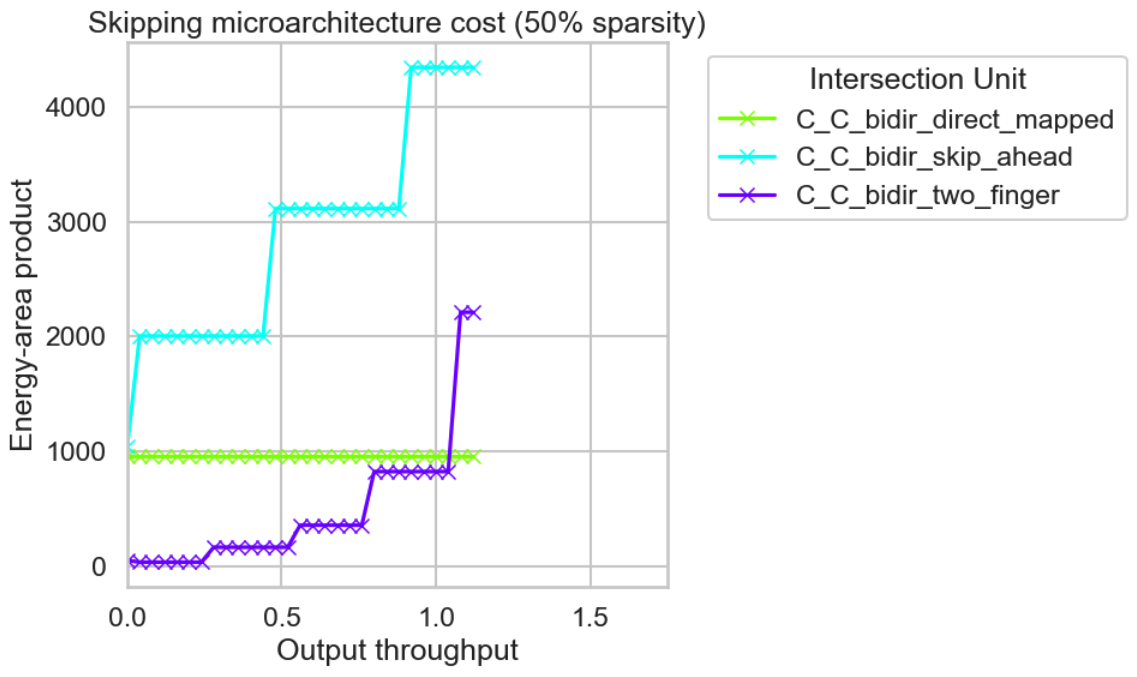
\includegraphics[width=\textwidth]{figures/skip_uarch_sparsity_50pct.png}
\caption{Comparison of energy-per-action/area product for 50\% sparse operands over a range of output throughput requirements..}
\label{fig:skip_uarch_sparsity_50pct}
\end{figure}

\begin{figure}[H]
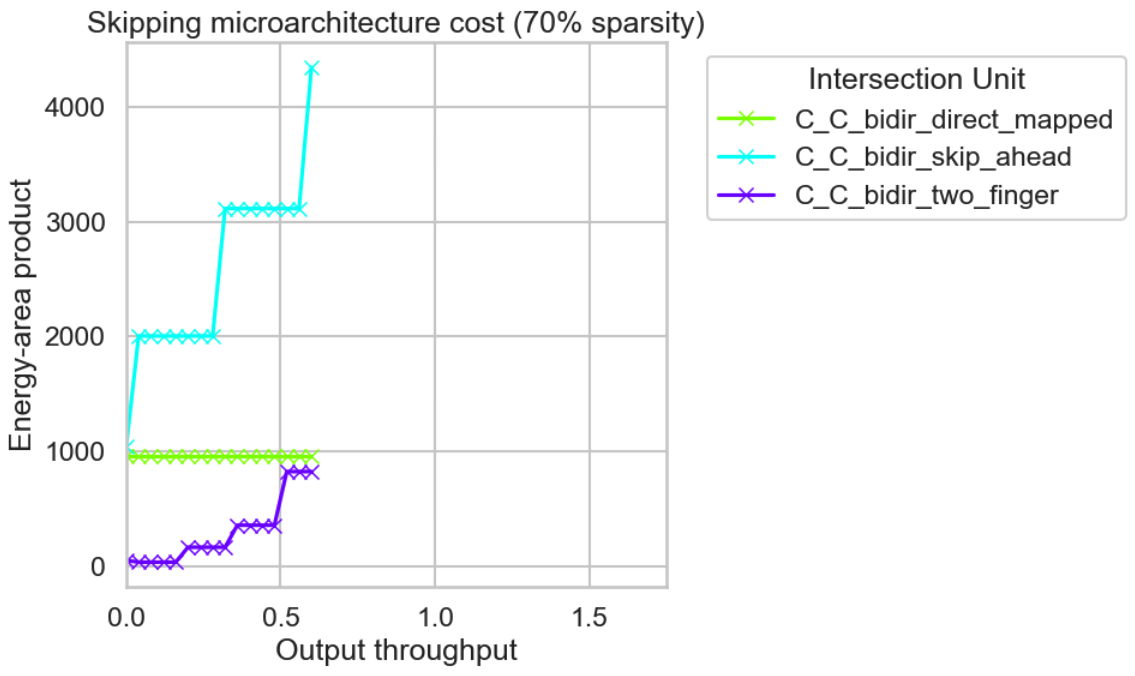
\includegraphics[width=\textwidth]{figures/skip_uarch_sparsity_70pct.png}
\caption{Comparison of energy-per-action/area product for 70\% sparse operands over a range of output throughput requirements..}
\label{fig:skip_uarch_sparsity_70pct}
\end{figure}

Figures~\ref{fig:skip_uarch_sparsity_30pct}, 
~\ref{fig:skip_uarch_sparsity_50pct}, and~\ref{fig:skip_uarch_sparsity_70pct} show how the skipping microarchitecture energy-per-action/area product scales with the output throughput requirement, for each type of intersection unit and for three different sparsity levels. In these figures, the number of pipeline stages is being optimized automatically during scale inference, in order to supply the required throughput. If an intersection unit is not able to supply the requisite throughput with any number of pipeline stages, then the corresponding curve will not have an energy-per-action/area product value associated with that throughput value.

These results suggest that in a SIMD 2 arithmetic scenario, the direct-mapped intersection unit would be a strong candidate for meeting throughput requirement while keeping energy and area low, for the following reasons:

\begin{itemize}
    \item For all sparsities shown, direct-mapped intersection unit has superior energy-per-action/area product \textit{at the highest supported output throughput.}
    \item As shown in Figure~\ref{fig:skip_uarch_pipe_2} Figure~\ref{fig:skip_uarch_pipe_5}, two-finger and skip-ahead intersection unit are efficiency-limited unless they are provisioned with multiple pipeline stages; as shown in Figures~\ref{fig:skip_uarch_sparsity_30pct},~\ref{fig:skip_uarch_sparsity_50pct}, and~\ref{fig:skip_uarch_sparsity_70pct}, this means that the energy-per-action/area product of these intersection units increases substantially with the output throughput design-point. In contrast, direct-mapped intersection unit requires only one pipeline stage regardless of throughput, and thus has uniform energy-per-action and area as the throughput requirement is scaled.
\end{itemize}


Note that in this case study, we are considering intersection units with vector pipelines; however, owing to an early decision to design microarchitecture models based on \textit{combinational unrolling} (Section~\ref{rtl}), the energy-per-action and area characterization results used here are based on combinational unrolling rather than \textit{pipelining}; this means that energy-per-action/area product values quoted in this section may be over-estimates for intersection units with more than one pipeline stage. This could explain the apparent non-linear scaling of two-finger intersection in Figures~\ref{fig:skip_uarch_sparsity_30pct},~\ref{fig:skip_uarch_sparsity_50pct}, and~\ref{fig:skip_uarch_sparsity_70pct}, as combinationally unrolling has non-linear overheads. 

However, it is likely that using energy-per-action and area characterization results based on pipelining, would not significantly change the outcome, because direct-mapped intersection would still have the best pipeline efficiency. Re-running these experiments with models based on pipelining, rather than combinational unrolling, is left for future work.
\chapter{Conclusion}
\label{chapter:conclusion}

A SAF microarchitecture taxonomy was developed and scoped to include format- and skipping- related SAF microarchitectures. A system for inferring low-level scale parameters and automatically sizing SAF microarchitecture components to satisfy workload requirements was also developed.

A library of RTL components was developed and characterized as a basis for creating analytical models of SAF microarchitecture primitives. These RTL models also serve as reference designs.

The SAFTools framework was developed to facilitate the end-to-end process of transforming declarative sparsity optimization specifications (in Sparseloop\cite{sparseloop} format) into SAF microarchitectures, and sizing SAF microarchitecture primitive components to satisfy inferred workload requirements.

A machine-learning method for modeling coordinate-payload bidirectional intersection unit transfer relations was developed, applied, and validated.

A potentially novel intersection unit variety, the direct-mapped intersection unit, was implemented in RTL, characterized, and modeled against other intersection unit varieties. Tentatively, it appears that direct-mapped intersection units may outperform other intersection unit varieties at serving high match throughput in SIMD arithmetic architectures while keeping energy and area low. However, affirming this result is contingent on further refinement of the SAF microarchitecture models developed in this work.

Future work should focus on (1) more in-depth validation of the whole work, (2) refinement of the models, and (3) further experimentation in order to confirm claims about direct-mapped intersection unit. Specific approaches to refining the models could include

\begin{itemize}
    \item Employing layout-level simulation to increase accuracy and capture more subtle overheads such as those resulting from wiring
    \item Where appropriate, implement vector-pipelined \textit{and} combinationall-unrolled variants of each model
    \item Providing options to use different types of pipelining; ensure that all models in a given experiment are configured to use the same form of pipelining.
\end{itemize}

It would be good to see validation and case studies which use Sparseloop alongside SAFTools to inform whole-design decisions.

Note that the full depth of modeling work which was done, was not validated. For example, the impact of clock period on energy and area was considered during characterization, but for brevity was not incorporated into the validation or case-studies.

If the relative benefit of utilizing direct-mapped intersection is supported by future work, this suggests that hashmap-based intersection units suggested in the ExTensor\cite{extensor} are also worth exploring: direct-mapped intersection units are essentially a special case of hashmap-based intersection units, in which the hashmap is the size of the dense rank.
\appendix
\chapter{Tables}

\begin{table}
\caption{Armadillos}
\label{arm:table}
\begin{center}
\begin{tabular}{||l|l||}\hline
Armadillos & are \\\hline
our	   & friends \\\hline
\end{tabular}
\end{center}
\end{table}

\clearpage
\newpage

\chapter{Modelscript syntax}

This section provides a brief overview of the \textit{modelscript} language that was created for this work and used to develop the SAFModel analytical model library.

\clearpage
\newpage

%% This defines the bibliography file (main.bib) and the bibliography style.
%% If you want to create a bibliography file by hand, change the contents of
%% this file to a `thebibliography' environment.  For more information 
%% see section 4.3 of the LaTeX manual.
\begin{singlespace}
\bibliography{main}
\bibliographystyle{plain}
\end{singlespace}

\end{document}

